% Dokumentenkonfiguration
\documentclass[a4paper,twoside,11pt,normalheadings,headsepline,footsepline,pointlessnumbers,aps,showpacs,showkeys,prd,superscriptaddress,byrevtex]{scrbook}
%\documentclass[a4paper,twoside,11pt,normalheadings,headsepline,footsepline,pointlessnumbers]{revtex4-1}
%\documentclass[a4paper,12pt,normalheadings,headsepline,footsepline,pointlessnumbers]{scrbook}
\usepackage{graphicx,amsfonts,bbm,makeidx,cite,amsmath}
\usepackage{dcolumn,ltxtable,url}
\usepackage[latin1]{inputenc}
\usepackage[ngerman,english]{babel}
\usepackage[T1]{fontenc}
\usepackage{graphicx}
\usepackage{mathrsfs}
\usepackage{bm}
\usepackage{epsfig}
\usepackage{subeqnarray}
\usepackage{upgreek}
\usepackage{afterpage}
\usepackage{color}
\usepackage{maybemath}
\usepackage{changepage}
\usepackage{doi}
\usepackage[square,numbers]{natbib}
\bibliographystyle{apsrev4-1}
\usepackage[titletoc]{appendix}

\usepackage{subfig}
\usepackage{pdfpages}
\usepackage{etaremune}
\usepackage[pdfpagelabels,hypertexnames=false]{hyperref}%hyprlinks in der pdf

% Curriculum vitae Konfiguration
% \usepackage[NoDate]{currvita}
% \renewcommand{\cvlistheadingfont}{\sffamily\bfseries\Large}
% \renewcommand{\cvlabelfont}{\itshape}
% \AtBeginDocument{\setlength{\cvlabelwidth}{54mm}}

% Koma Script Konfiguration
\areaset[18mm]{14cm}{26cm}              % A4 paper and letter paper      
\deffootnote[1em]{1em}{1em}{\textsuperscript{\normalfont\thefootnotemark}}
\setcapindent{0pt}
\renewcommand\bibname{References}
\renewcommand{\capfont}{\small\sffamily}
% \renewcommand{\caplabelfont}{\small\sffamily\bfseries}
\renewcommand{\caplabelfont}{\small\sffamily}
\renewcommand{\headfont}{\sffamily\large}
% \renewcommand{\pnumfont}{\sffamily\bfseries\large}
\renewcommand{\pnumfont}{\sffamily\large}
\setcounter{secnumdepth}{3}
\setcounter{tocdepth}{2}


% dcolumn Konfiguration
\newcolumntype{d}{D{.}{.}{-4}}

% Picture Konfiguration
\setlength{\unitlength}{1cm}

% LaTeX Konfiguration
\setlength{\itemsep}{100pt}
\newcommand{\graphsize}{12cm}
\newcommand{\smallgraphsize}{6cm}
%\newcommand{\href}[2]{\url{#2}}
\let\onlinecite=\cite
\makeindex


%%%%%%%%%%%%%%%%%%%%%%%%%%%%%%%%%%%%%%%%%%%%%%%%%%%%%%%%%%%%%%%%%%%%%%%%%%%%%%%%%%%%%%%%%%%%%%%%%%%
\begin{document}
%
\frontmatter
\begin{titlepage}
\begin{center}
  \renewcommand{\baselinestretch}{1.50}
  {\bfseries
    Dissertation \\
    submitted to the \\
    Combined Faculty of Natural Sciences and Mathematics \\
    of Heidelberg University, Germany \\
    for the degree of \\
    Doctor of Natural Sciences
    \par
  }
  \vfill
  {\bfseries
    Put forward by \\
    \vspace{0.5\baselineskip}
    {\Large Kamil Dzikowski} \\
    \vspace{0.5\baselineskip}
    born in Wroc\l aw, Poland \\
    Oral examination: October 20$^{\textrm{th}}$, 2021
    \par
  }
\end{center}
\end{titlepage}

%% Titlepage
\begin{titlepage}
\begin{center}
  \renewcommand{\baselinestretch}{1.50}
  \vspace*{1.5\baselineskip}
  \bfseries
  {\huge \sffamily
  Effective charge model for multi-electron atoms
  \par}
  \vfill
  \large
  \begin{tabular}{lp{0.5cm}l}
  Referees: && PD Dr. Natalia S Oreshkina \\
            && Prof. Dr. Joerg Jaeckel
  \end{tabular}
\end{center}
\end{titlepage}

%%% Local Variables:
%%% mode: latex
%%% TeX-master: "../doc"
%%% End:

\cleardoublepage
\thispagestyle{empty}
\begin{otherlanguage}{ngerman}
{\small
  \begin{center}
    \textbf{Zusammenfassung}
  \end{center}

  \noindent Das k\"urzlich vorgeschlagene Effektivladungsmodell (ECM) ist ein neuartiger Ansatz, um vollst\"andig analytische Ann\"aherungen an die beobachtbaren Eigenschaften von Mehrelektronenatomen und -ionen zu erhalten. Es verwendet einen wasserstoff\"ahnlichen Basissatz mit einem einzigen Parameter, der als effektive Ladung bezeichnet wird, um eine St\"orungstheorie zu konstruieren. Die zugeh\"orige St\"orungsreihe konvergiert schnell, ber\"ucksichtigt auf nat\"urliche Weise Korrelationseffekte und erm\"oglicht eine effiziente Berechnung aller nachfolgenden Korrekturen. In dieser Arbeit vergleichen wir die Genauigkeit der durch das ECM erzeugten analytischen N\"aherungen mit Ergebnissen anderer gebr\"auchlicher Methoden, wie der Hartree-Fock-Methode und dem Thomas-Fermi-Modell, sowohl innerhalb der relativistischen als auch der nicht-relativistischen Quantenmechanik. Zu diesem Zweck werten wir Grundzustandsenergien, Energien angeregter Zust\"ande und Ionisationsenergien sowie eine Vielzahl anderer atomarer Eigenschaften wie Elektronendichten, Streufaktoren, Photoionisationsquerschnitte und \"Ubergangswahrscheinlichkeiten f\"ur ein breites Spektrum von Systemen,
von neutralen Atome bis zu hochgeladenen Ionen, aus. Wir zeigen auch, wie die Greensche Funktion des Wasserstoffatoms analytisch integriert werden kann, um eine effiziente Berechnung der ECM-Korrekturen zweiter Ordnung zu erm\"oglichen. Schlie\ss lich untersuchen wir verschiedene zus\"atzliche Effekte, die die Genauigkeit der ECM-N\"aherungen korrigieren, insbesondere solche, die durch die Breit-Wechselwirkung, durch endlichen-Kerngr\"o\ss e-Effekte und durch die Vakuumpolarisation hervorgerufen werden. Da die Genauigkeit der ECM-Approximationen zweiter Ordnung bereits mit Ergebnissen eines Hartree-Fock-Ansatzes mit mehreren Konfigurationen vergleichbar ist, k\"onnen wir uns vorstellen, dass das ECM das Thomas-Fermi-Modell, f\"ur alle Anwendungen, in denen es noch verwendet wird ersetzen kann.} %dass das ECM andere Modelle vergleichbarer Komplexit\"at, wie zum Beispiel das Thomas-Fermi-Modell, f\"ur alle Anwendungen, wo es noch genutzt wird ersetzen kann.}
\end{otherlanguage}

{\small
  \begin{center}
    \textbf{Abstract}
  \end{center}

  \noindent The recently proposed effective-charge model (ECM) is a novel approach to producing fully analytical approximations to the observable characteristics of multi-electron atoms and ions. It employs a hydrogen-like basis set with a single parameter, called effective charge, for the construction of perturbation theory. The associated perturbation series converges fast, includes correlation effects in a natural way and enables an efficient calculation of all subsequent corrections. This work compares the accuracy of the analytical approximations produced by the ECM to results of other commonly used methods, such as the Hartree-Fock method and the Thomas-Fermi model, within both relativistic and non-relativistic quantum mechanics. For this purpose, ground state, excited state and ionization energies are evaluated, as well as a wide range of other atomic characteristics, such as electronic densities, scattering factors, photoionization cross-sections and transition probabilities, for a wide range of systems, from neutral atoms to highly charged ions. It is also shown how the Green's function of the hydrogen atom can be integrated analytically, allowing for an efficient calculation of the second-order ECM corrections. Finally, various additional effects that correct the accuracy of the ECM approximations are investigated, in particular those originating from the Breit interaction, finite-nuclear-size effects and vacuum polarization. Given that the accuracy of the second-order ECM approximations is already comparable with results obtained using a multi-configuration Hartree-Fock approach, we envisage that the ECM can replace the Thomas-Fermi model for all applications where it is still utilized.}

%%% Local Variables:
%%% mode: latex
%%% TeX-master: "../doc"
%%% End:

\cleardoublepage
\mainmatter

\tableofcontents

\chapter*{List of publications}

Within the framework of this thesis, the following articles have been published
in peer-reviewed journals:
\begin{itemize}
    \item  K D Dzikowski and O D Skoromnik, \textit{A generating integral for the matrix elements of the Coulomb Green's function with the Coulomb wave functions}, Journal of Mathematical Physics \textbf{61}, 032103 (2020).
    \item  K D Dzikowski, O D Skoromnik, I D Feranchuk, N S Oreshkina and C H Keitel, \textit{Relativistic effective charge model of a multi-electron atom}, Journal of Physics B: Atomic, Molecular and Optical Physics \textbf{54}, 115002 (2021).
\end{itemize}

\chapter{Introduction}
\addtocontents{toc}{\contentsline{chapter}{Introduction}{\protect\pageref{annotation}}}

\section{Atoms}

Atoms (from ancient Greek $\alpha \tau o \mu o \varsigma$ meaning uncutable) are the building blocks of all chemical elements and among the most intensely studied systems in all of physics. Their existence has been speculated since antiquity~\cite{pullman2001atom}, but no testable atomic theory existed until the early 19th century, when the law of definite proportions was laid out in chemistry~\cite{dalton2010new} and the relation between thermodynamics of gases and statistical physics was realised~\cite{thomson1816annals}. The first experimental observation of atoms came in the form of discrete absorption lines in the solar spectrum~\cite{Wollaston1802, von1817bestimmung} that could later be connected to laboratory analysis of gases~\cite{Angstrom1862} to identify the signatures of specific chemical elements. Similar experiments, including those conducted in Heidelberg~\cite{KirchhoffBunsen, KirchhoffBunsen2}, led to the development of spectroscopy which to this day remains a primary tool of investigating physics at smallest scales~\cite{workman1998applied}.

Theoretical understanding of the mechanics of atoms and the origin of their spectral lines was to prove more challenging. Despite the discovery of the electron in 1897 in cathode ray tube experiments~\cite{thomson1897xl}, early attempts remained purely empirical, such as the famous Rydberg formula for hydrogen~\cite{Balmer1885}. It wasn't until Rutherford showed in 1911 that most of the mass of any atom is concentrated in the positively charged nucleus~\cite{Rutherford1911},
that physical models of the inner structure of atoms could be developed. The first successful one, was the model of hydrogen by Bohr~\cite{bohr1913constitution} and its subsequent extension by proper quantization of angular momentum by Sommerfeld~\cite{Sommerfeld1916}. Generalising these to multi-electron atoms only became possible in 1925 with the advent of modern quantum mechanics in the form of the Schr\"{o}dinger~\cite{1926PhRv28.1049S} and, later, Dirac equations~\cite{rspa.1928.0023}. The latter was a particularly significant development, as by requiring consistency with Einsteins theory of relativity~\cite{bjorken1964relativistic} it naturally incorporated the spin of the electron, which in turn explained~\cite{Uhlenbeck1925} the splitting of absorption lines in external field known as the Zeeman effect~\cite{zeeman1897xxxii}.

The next important development came with the experimental discovery of the Lamb shift~\cite{PhysRev.72.241}, that is, an energy difference between states predicted by the Dirac equation to be degenerate, and its subsequent theoretical explanation within the theory of quantum electrodynamics
(QED)~\cite{PhysRev.73.416}. %What is the explanation?
The latter eventually lead to some of the most precise predictions in the history of physics, such as the value of the $g$-factor of the electron, which has been calculated~\cite{calculatedgfactor} and measured~\cite{PhysRevLett.97.030801} to below one-part-per-trillion accuracy. 

To this day, atoms remain a vital tool in the study, both theoretically and experimentally, of quantum field theories~\cite{Rafelski2017}, light-matter interactions~\cite{Shafir2009} and determination of physical constants, such as the fine structure constant~\cite{PhysRevLett.97.030802, erratum}. However, despite great progress in their theoretical description, they represent some of the simplest and most evident examples of physical systems that lack analytical solutions. Only the smallest, hydrogen atom with its single electron orbiting the nucleus can be solved exactly, as a two-body problem within both Schr\"{o}dinger and Dirac quantum theories. Adding one more electron to create helium already makes it impossible, mirroring the inherent difficulty of three-body problems in other areas of physics. However, while a system of two planets orbiting a star may not have an analytic solution due to inherent chaos that prevents the existence of stable orbits, all helium atoms in the universe have exactly the same physical properties indicating the existence of some well-defined - even if too complex for us to express - solutions.

 The computational complexity involved in describing multi-electron atoms can be visualized by considering the maximum amount of information contained in an arbitrary wavefunction. In general, an $n$-electron wavefunction in 3 dimesions is a function of $3n$ variables that can involve arbitrary correlations. This means that computational complexity increases exponentially with the number of electrons. For a simplified illustrative example, while the hydrogen atom can be numerically described on a 3D grid using 1 MB of data (50 points in each dimension with 2 bytes each - 1 for the real part and 1 for the imaginary part), this number goes up to 1 TB  for helium and 1 exabyte for Lithium, just to describe its three electrons. By the time we reach silicon with its 13 electron, the volume of the required hard drive exceeds $10^{40}$ sun volumes! \footnote{The author is greatful to Z. Harman for this example.}

Since the advancement in computational power cannot on their own overcome those difficulties, approximate methods remain the primary tool.

\section{Atomic calculations}

In the early days of quantum mechanics, multi-electron atoms were described using empirical modifications to the Bohr model of hydrogen, such as quantum defects~\cite{Seaton_1983}, or Slater orbitals~\cite{slater_atomic_1930}, with empirical principles such as the Moseley's law~\cite{14786441308635052} remaining popular. 

One of the first successful ideas for describing multi-electron atoms \textit{ab-initio}, that is, without experimental input, was the semi-classical Thomas-Fermi (TF) model. It was developed in 1927~\cite{1927PCPS2542T}, specifically as a method of approximating the distribution of electrons in an atom. The main idea is to look for electron density, rather than the wavefunction. If one can find a reasonable guess on the dependence of binding energy on the electron density (known as the density functional), then the form of the latter can be obtained by simply minimizing the energy. This effectively becomes a 1-dimensional problem (assuming the nuclear potential is spherically symmetric), rather than the 3n-dimensional problem of finding the multi-electron wavefunction.

Despite being rather inaccurate in its original form and failing to reproduce shell structure of atoms or the molecular bonding, the model remained relevant due to its simplicity. In subsequent decades, increasingly sophisticated arguments~\cite{1927PCPS2542T} have refined the form of the kinetic energy functional, until in 1964 Kohn and Hohenberg showed that the ground state of any electronic system is uniquely determined by the corresponding electronic density~\cite{PhysRev.136.B864}. This laid the foundations for Density Functional Theory that has since found numerous applications, particularly in the study of solids. Despite its problems, the Thomas-Fermi model is still used in modern computer codes, for example for plasma simulations~\cite{ciricosta_direct_2012, starrett_thomas-fermi_2017, dyachkov_region_2016} where a large number of repeated evaluations of electronic density need to be performed.
  
Obtaining a more accurate description of multi-electron atoms required methods capable of approximating the entire multi-electron wavefunction. The most important insight was proposed already in 1927 by D. R. Hartree~\cite{hartree_1928}, who suggested to deal with the non-linear nature of the Schr\"{o}dinger equation by an iterative process. In 1935, it was reformulated into its modern form in terms of Slater determinants~\cite{rspa19350085}, known as the Hartree-Fock (HF) method, but didn't become popular until the advent of computers, as it requires comparatively intensive computations. The main idea is to make an initial guess on the shape of occupied atomic orbitals, and then use them to obtain an effective potential acting on each electron individually. This is then used to find a new improved orbital occupied by each electron. This process is repeated until the potential produced by the electrons is consistent with the one used to find their distribution. For this reason it is often referred to as the self-consistent field method.

The Hartree-Fock procedure has since been refined to include effects of electron-electron correlation using a wide range of methods, known collectively as post-Hartree-Fock methods. These include configuration interaction~\cite{Tup2003OS} and coupled clusters~\cite{bostock_fully_2011} among others. %(what others?!).
Many of them have been incorporated into various software packages such as GRASP2k~\cite{jonsson_new_2013, DYALL1989425} and FAC~\cite{FAC}, along with further corrections coming from quantum electrodynamics and improved nuclear models. Furthermore, methods based on the Hartree-Fock procedure can easily be adapted to solve a much broader class of problems, and so they have found widespread use in describing not only multi-electron atoms~\cite{fischer1977hartree}, but also molecules~\cite{puchalski_relativistic_2017, jensen2007introduction} and atomic nuclei~\cite{TARBUTTON19681}. However, in practice the HF method is still too computationally intensive for many practical applications and further approximations are often required - most importantly, the separate treatment of inner (core) and outer (valence) electrons~\cite{pseudopotentials}.

After the Dirac equation was proposed in 1928, relativistic versions of both the Thomas-Fermi and Hartree-Fock methods have been developed. These are referred to as Thomas-Fermi-Dirac model (TFD) and Dirac-Hartree-Fock method (DHF) respectively.

\section{Analytical methods of atomic calculations}

One important feature of the methods described in the previous section, is that they rely heavily on numerical calculations and do not produce analytical expressions for observable atomic properties. For this reason, simple analytical models are still actively developed
\cite{TATEWAKI201849, gomez_simple_2019, SimpleHey} for applications, where certain
level of precision has to be sacrificed for improved computation time,
such as in computational plasma physics~\cite{lee_model_1987, chung_flychk:_2005}, X-ray scattering and diffraction~\cite{hau2012high, feranchuk_new_2002} or crystallography~\cite{toraya_new_2016}. Most often these come in the form of semi-empirical models, such as
those based on quantum defects of Rydberg atoms~\cite{foot2005atomic}, or screened hydrogen~\cite{hau2012high}.

From a purely mathematical point of view, the main difficulty in describing multi-electron atoms is that the corresponding equations are non-linear, preventing the existence of closed-form solutions. Approximate analytical expressions can however be obtained using perturbation theory, which is a formal way of quantifying the difference between a complicated problem and a simplified, exactly solvable one. In the case of multi-electron atoms, one can solve the non-interacting problem (i.e. hydrogen-like) exactly and treat the electron-electron repulsion as a perturbation. This is often referred to as the $1/Z$ expansion, where $Z$ stands for the charge of the nucleus. A variational procedure for a numerical computation of coefficients for two-electron atoms within Schr\"odinger theory has been first developed by A. Hylleraas in 1930~\cite{1930ZPhy6209H}. In subsequent decades his approach was greatly refined, with over 300 orders of perturbation computed within Schr\"dinger theory \footnote{This approach doesn't generalize naturally to the Dirac theory, as it requires explicit dependence on nuclear charge.} for two-electron ions with high accuracy by 1990~\cite{PhysRevA.41.1247} .

The main drawback of the the $1/Z$ expansion, is that analytical expressions for wavefunctions exist only in the zeroth order, which offers relatively low accuracy. At the same time the calculation of higher orders quickly becomes computationally expensive, especially for larger atoms. Both of these issues can be improved upon with the use of the recently developed~\cite{Skoromnik_2017} Effective Charge Model (ECM). Its main premise is an improvement of the convergence rate of the perturbation series by the introduction of a single variational parameter - the effective nuclear charge $Z^*$. The intuitive idea of an effective nuclear charge is based on the notion that
electrons ``screen'' each other from the nucleus thus lowering the
Coulomb attraction to some ``effective'' value. The numerical value of the effective charge can then be chosen for any electronic configuration in a way that speeds up the convergence of the perturbation series, thus greatly increasing the accuracy of the analytical zeroth-order approximation. 

The idea of an effective nuclear charge resulting from electronic screening is itself not new. In fact, it was suggested by Slater already in 1930~\cite{slater_atomic_1930}. It was originally envisioned as a way of approximating multi-electron atoms by adjusting hydrogen-like wavefunctions of individual atomic orbitals according to a set of simple, empirically motivated rules. In subsequent decades the effective nuclear charges were adjusted from their original values proposed by Slater, in order to better reproduce experimental data, or results of numerical calculations. In the 1960s they were calculated for all orbitals of all neutral atoms by Clementi \textit{et al.}\cite{clementi1963atomic, clementi1967atomic}, by the best fit to the results of a HF-like self-consistent numerical method. These are however crucially distinct in both definition and numerical value, from the effective charge used in ECM. The latter is introduced in a mathematically rigorous way as a parameter of the model, with values determined purely from theoretical considerations, without any empirical input.

In the context of the ECM, the introduction of effective charge means adjusting the basis set in which the perturabative calculation is performed i.e. the set of hydrogen-like functions. By keeping the value of $Z^*$ identical for all single-electron wavefunctions of a given electronic configuration, the hydrogen-like basis remains orthonormal and the perturbation series well-defined. Furthermore, it allows all higher orders of perturbation to be expressed in terms of the hydrogen-like Green's function, which has a known analytical closed form. Similar techniques have also been used successfully to deal with other computationally challenging systems, e.g. to obtain analytical approximations to eigenvalues of some non-hermitian Hamiltonians~\cite{articleOleg}.

In this work, we show how the ECM can be used to obtain analytical approximations to both global and local atomic characteristics of all atoms and ions, in both ground and excited states. In particular, we investigate electronic densities, scattering factors, transition probabilities, ionization energies and photoionization cross-sections within both Schr\"odinger and Dirac theories. We show that the leading-order approximation is enough to obtain correct ordering of the energies of electronic configurations for all atoms of the periodic table. Furthermore, we investigate to what extent the accuracy can be improved, by the inclusion of higher order corrections to energies and wavefunctions.

We emphasize again that our aim is to keep the ECM an \textit{ab-initio} theory, in contrast to many modern approximation schemes that contain parameters fitted to the results of HF calculations~\cite{Koga1997} or experimental data, such as the interpolation of
X-ray measurements~\cite{genoni_can_2017}. It also means, that the ECM avoids a lot of the numerical problems associated with local minima of the parameter space, that can make the convergence of the semi-empirical methods dependent on starting conditions~\cite{PhysRevA36467}. At the same time it is much simpler and less computationally intensive than the standards methods used for high precision atomic calculations.

Most importantly, contrary to the TF model and methods based on the HF procedure, all expressions for atomic characteristics calculated with the ECM are fully analytical. Therefore, we suggest that the ECM can replace the TF model in all applications requiring rapid computations, including as an initial approximation for the self-consistent field methods for which convergence is strongly dependent on the choice of the trial wavefunctions.

\begin{table}
    \centering
    \begin{tabular}{l|ll}
        Unit & Expression & Value in SI \\
        \hline \hline
        mass & $m_e$ & $9.1094 \times 10^{-31}$ kg\\
        action & $\hbar$ & $1.0546 \times 10^{-34}$ Js \\
        charge & $e$ & $1.6022 \times 10^{-19}$ C\\
        permitivity & $1/k_e$ & $1.1127 \times 10^{-10}$ F/m\\
        length & $a_0$ & $5.2918 \times 10^{-11}$ m \\
        energy & $E_h$ & 27.211 eV \\
        momentum & $\hbar/a_0$ & $1.9929 \times 10^{-24}$ kg m/s\\
        electric dipole moment & $e a_0$ & $8.4784 \times 10^{-30}$ Cm\\
        magnetic dipole moment & $e \hbar/m_e$ & $1.8548 \times 10^{-23}$ J/T \\
        force & $\alpha^2 m_e c^2 /a_0$ & $8.2387 \times 10^{-8}$ N \\
        time & $\hbar/(\alpha^2 m_e c^2)$ & $2.4189 \times 10^{-17}$ s \\
        \hline
    \end{tabular}
    \caption{Some of the most relevant atomic units. Five significant figures are given, but in most cases many more digits are known~\cite{1959Natur1841559S}. $E_h$ denotes the Hartree energy.}
    \label{tab:units}
\end{table}

\section{Outline}

This thesis is organised in the following way. In chapter \ref{ch:Methods}, we discuss the theoretical framework and practical realisation of the Thomas-Fermi model, the Hartree-Fock method and the $1/Z$ perturbation expansion. In chapter \ref{ch:basics}, we outline the standard approach to solving the Schr\"odinger and Dirac equations for the hydrogen atom and provide all necessary formulas and definitions required for the consistency of subsequent chapters. In chapter \ref{ch:ECM}, we define the hydrogen-like basis set and present the leading-order relativistic and non-relativistic ECM approximation, along with the respective calculations of effective charge. In chapter \ref{ch:secondECM}, we show how the Coulomb and Dirac Green's functions can be used to derive all formulas expressing second-order corrections to the ECM, including those involving electron-electron correlation. In chapter \ref{ch:IntGreen}, we discuss the possibilities and limitations of the analytical and numerical evaluation of second-order corrections and outline the derivation of corresponding formulas related to the analytical integration of the Coulomb Green's function. This chapter is heavily based on the research we previously published as~\cite{Dzikowski_2020}. In chapter \ref{ch:Applications}, we discuss the accuracy of the ECM by evaluating analytical approximations to a wide range of properties of atoms and ions and compare the results to the TF and HF methods. Both this chapter, as well as chapter~\ref{ch:ECM}, present research we previously published in~\cite{Dzikowski_2021}. In chapter \ref{ch:Improvements}, we show that the leading-order ECM can be used to accurately estimate the most important QED and nuclear corrections to atomic energies. In particular, those related to the Breit interaction, finite-nuclear-size effect, and vacuum polarization. In chapter \ref{ch:Conclusions}, we provide conclusions and outlook.

Larger data tables, as well as the details of derivations of analytical formulas and algorithms used in numerical computations, can be found in the Appendix.

\section{Units and abbreviations}

Atomic units are employed throughout this work. This means that the reduced Planck constant, elementary charge, electron mass and the Coulomb constant are set to unity:
\begin{align*}
    \hbar = 1,\\
    e = 1,\\
    m_e = 1, \\
    k_e = 1.
\end{align*}
Note that this also makes the Bohr radius equal to unity: $a_0=1$ and the speed of light becomes equal to the inverse of the fine structure constant $c= \frac{1}{\alpha} \approx 137.036$. The translation to SI units is given in table \ref{tab:units}. 

Major abbreviations used throughout this thesis:
\begin{align*}
   \rm{ECM} &- \text{effective charge model}\\
   \rm{D}\text{-}\rm{ECM} &- \text{relativistic effective charge model} \\
    \rm{HF} &- \text{Hartree-Fock}\\
    \rm{DHF} &- \text{Dirac-Hartree-Fock}\\
    \rm{TF} &- \text{Thomas-Fermi} \\
    \rm{TFD} &- \text{Thomas-Fermi-Dirac} \\
    \rm{CI} &- \text{configuration interaction} \\
    \rm{DFS} &- \text{Dirac-Fock-Sturm} \\
    \rm{HFS} &- \text{Hartree-Fock-Slater} \\
    \rm{RCGF} &- \text{reduced Coulomb Green's function} \\
    \rm{RCDGF} &- \text{reduced Coulomb-Dirac Green's function} \\
    \rm{HCI} &- \text{highly charged ions}
\end{align*}



\chapter{Overview of existing methods}
\addtocontents{toc}{\contentsline{chapter}{Methods}{\protect\pageref{annotation}}}
\label{ch:Methods}

This chapter presents some of the well-established methods of approximating the wavefunctions of multi-electron atoms. The Thomas-Fermi model that eventually led to the development of Density Functional Theory, the Hartree-Fock method that forms the basis of many modern high-precision atomic calculation schemes and the perturbation series in the inverse of the nuclear charge.

\section{The Thomas-Fermi model}
\label{sec:TF}

The main idea of the TF model is to look for the form of electron density, as a function of space $n(\vec{r})$, rather than the multi-electron wavefunction, as a function of the positions of individual electrons: $\Psi(\vec{r_1} ... \vec{r_N})$. This is done by writing the total energy of the electron cloud as a functional of the electron density, and looking for its minimum: 
\begin{equation}
     E[n(\vec{r})] = E_{kin}[n(\vec{r})] + U_{eN}[n(\vec{r})] + U_{ee}[n(\vec{r})],
\end{equation}
where $U_{eN}$ and $U_{ee}$ are the electron-nucleus and electron-electron potential energies respectively.

Assuming that electrons are uniformly distributed in phase space up to the Fermi momentum, with the classical expression for kinetic energy $E_{kin} = p^2/2$, one can obtain the density functional as~\cite{lundqvist2013theory}: 
\begin{equation} \label{TFenergy}
     E[n(\vec{r})] = C_{\rm{kin}}\int n(\vec{r})^{5/3} d \vec{r} + \int V_{N}(\vec{r})n(\vec{r}) d \vec{r} + \frac{1}{2} \int \frac{n(\vec{r_1}) n(\vec{r_2})}{|\vecr{r_1}-\vec{r_2}|} d\vec{r} d\vec{r_2},
\end{equation}
where $V_N$ is the nuclear potential and $C_{\rm{kin}}$ is a numerical constant related to the volume of occupied phase space, in this case: $C_{\rm{kin}} \approx 2.8712$.

The task is then to minimize the energy, while keeping the number of electrons $N$ constant:
\begin{equation}
    \int n(\vec{r})d \vec{r} = N.
\end{equation}

This can be achieved using a Lagrange multiplier $\mu$, called chemical potential, given by:
\begin{align}
\mu = \frac{5}{3} C_{kin} n(\vec{r})^{2/3} + V(\vec{r}),
\end{align}
where $V$ is the total (effective) potential:
\begin{align}
V(\vec{r}) = V_{N}(\vec{r}) + \int \frac{n(\vec{r_2})}{|\vec{r_2}-\vec{r}|} d\vec{r_2},
\end{align}
and looking for the form of $V(\vec{r})$ that corresponds to a stationary point. The numerical value of $\mu$ is related to the difference between the nuclear charge and the number of electrons, so that $\mu = 0$ for neutral atoms and $\mu < 0$ for positive ions.

In the case of a spherically symmetric nucleus, the total potential becomes a one-dimensional function $V(\vec{r}) = V(r)$. For the case of a point-like nucleus $V_N = -\frac{Z}{r}$, the effective potential can be expressed as:
\begin{align}
V(r) = \mu - \frac{Z}{r} \phi \left(\frac{r}{b}\right),~~~~~~~~~~b=\frac{1}{4}\left(\frac{9\pi^2}{2Z}\right)^{1/3}.
\end{align}
The potential $V(r)$ is then a stationary point of \eqref{TFenergy} whenever the function $\phi(r)$ satisfies the so-called Thomas-Fermi equation~\cite{davis1962introduction}:
\begin{equation} \label{TFequation}
    \frac{\partial^2 \phi(r)}{\partial r^2} = \frac{\phi^{3/2}(r)}{\sqrt{r}},
\end{equation}
with boundary conditions $\phi(0)=1$ and $\phi(+\infty)=0$.

This deceptively simple looking differential equation has no analytical solution and is plagued by a somewhat famous numerical problem. In order to propagate a numerical solution of \eqref{TFequation} from the origin, it is necessary to know the initial slope $\phi'(0)$, which cannot be calculated analytically. Furthermore, even slight deviation from its critical value can lead to an entirely wrong behaviour. If the value of the initial slope is bigger than the critical value, the numerically propagated $\phi(r)$ diverges at a finite $r$ and if it's smaller, it crosses the real line whereby becoming complex (see figure~\ref{TFfig}). An algorithm for calculating the critical value of $\phi'(0)$ was first developed by Ettore Majorana in 1928~\cite{1.1484144}, and considerable effort has since gone into improving it, including in recent years~\cite{LIU2015251,PARAND2017624,pub1041457795}.
\begin{figure} [t] 
	\centering
	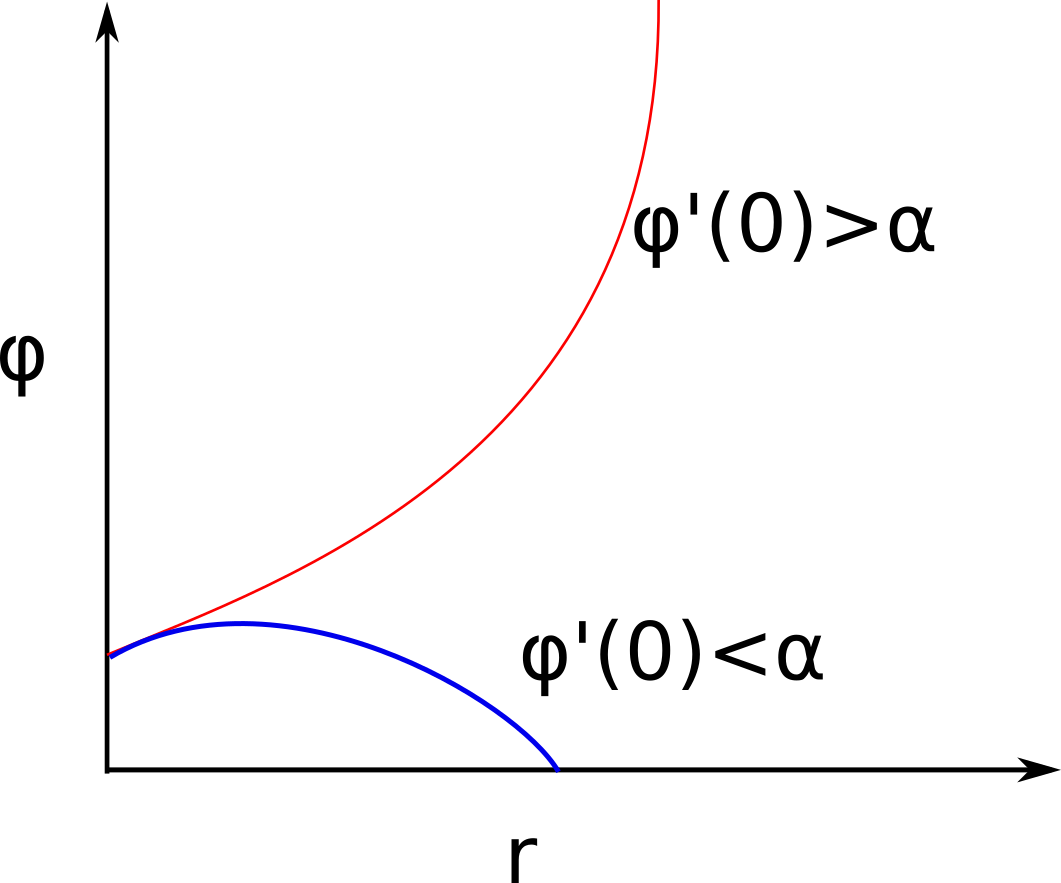
\includegraphics[width=80mm]{Graphs/TF.png} 
	\caption{Pictorial representation of the numerical difficulties associated with finding normalizable solutions of the Thomas-Fermi equation. The initial value $\phi(0)$ is given, but the initial slope $\phi'(0)$ needs to be found by trial and error. If the value is higher that the critical value $\alpha$, the numerically propagated solution diverges. If it is lower, the solution hits the real line and becomes complex.} \label{TFfig}
\end{figure}

\section{The Hartree-Fock method}

The main idea of the HF method is to look for a distribution of electrons self-consistent with a field that it generates. The first step is to specify the ground state configuration, that is, a set of occupied electron orbitals $\phi_i$. Then an initial approximation to the shape of all of those occupied single-electron orbitals is needed. This can be done using the Thomas Fermi model, or by solving the corresponding problem without the electron-electron interaction.
In order to ensure anti-symmetry, the total multi-electron wavefunction is represented by a Slater determinant of single-electron orbitals:
\begin{equation} \label{HFdet}
  \Phi(\vec{r_1}, \vec{r_2} ... \vec{r_N}) = \frac{1}{\sqrt{N!}}
   \left| \begin{matrix} \phi_1(\vec{r_1}) & \phi_2(\vec{r_1}) & \dots & \phi_2(\vec{r_1}) \\
    \vdots & & \ddots &  \\ 
    \phi_1(\vec{r_N}) & \phi_2(\vec{r_N})& \dots & \phi_N(\vec{r_N})  \end{matrix} \right|.
\end{equation}

The influence of electron-electron interaction is then taken into account using the mean-field approximation, meaning that any given electron is assumed to occupy a bound state in the potential formed by all of the other electrons and the nucleus. This means that for the $i^{\rm{th}}$ electron we can find the so-called Fock operator $\widehat{F}_i$ given by~\cite{560430312}:
\begin{equation}
    \widehat{F}_i = \widehat{H}_i+\sum_j^n (\widehat{J}_{ij} - \widehat{K}_{ij}),
\end{equation}
where $\widehat{J}_{ij}$ and $\widehat{K}_{ij}$ are the Coulomb and exchange operators describing the interaction between the $i^{\rm{th}}$ and $j^{\rm{th}}$ electrons, and $\widehat{H}_i$ is the single particle Hamiltonian of the $i$ electron, including it's kinetic energy and interaction with the nucleus. If the relativistic version of $H_i$ is used, then the method is referred to as Dirac-Hartree-Fock (DHF) procedure.

Each of the Fock operators can then be diagonalized:
\begin{equation}
    \widehat{F}_i \phi_i = E_i \phi_i,
\end{equation}
to obtain a new set of occupied orbitals $\phi_i$. This process is repeated until a specified level of accuracy is reached. The schematic representation of this algorithm is presented in figure~\ref{HFalgo}.

When implementing the HF procedure in a computer program, in order to efficiently diagonalize the set of Fock operators $\widehat{F}_i$, the occupied orbitals $\phi_i$ are typically expanded in a basis, that allows for rapid evaluation of Coulomb and exchange integrals. This means that the whole computation is reduced to the repeated calculation of the expansion coefficients of the orbitals. Popular choices of basis sets include Gaussian functions, B-splines,~\cite{FROESEFISCHER20111315} and Sturmian functions~\cite{sturmian}.

The variational principle~\cite{epstein2012variation} tells us, that the expectation value of the Hamiltonian with any wavefunction is higher than the ground state energy, which means that the Hartree-Fock procedure always provides an upper bound on the ground state energy (this is not necessarily the case for excited states~\cite{LandauQM}).

\begin{figure} [t] 
	\centering
	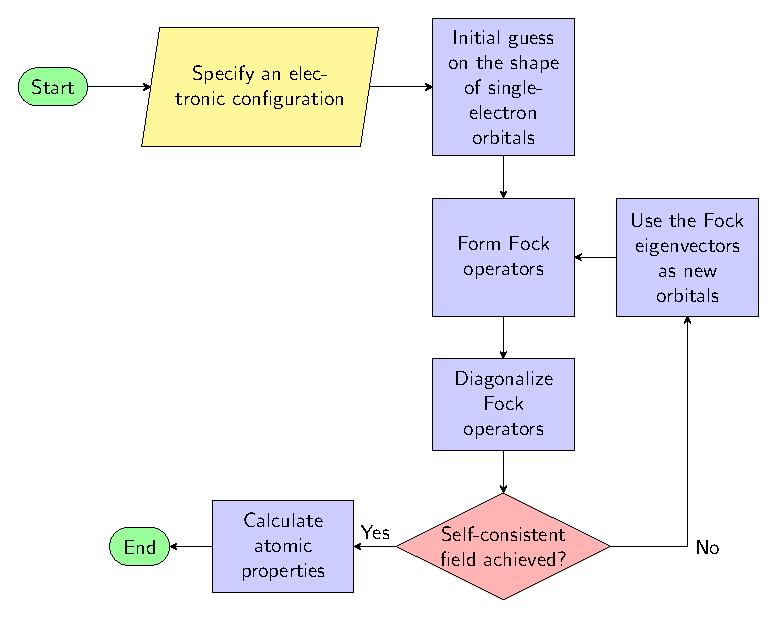
\includegraphics[width=119mm]{Graphs/HFalgorithm.pdf} 
	\caption{Pictorial representation of the basic algorithm behind using the HF method to calculate properties of multi-electron atoms.} \label{HFalgo}
\end{figure}

Because of the mean-field approximation described above, all electron-electron correlation beyond the anti-symmetry relation is neglected. This is typically the main source of uncertainty in the Hartree-Fock procedure. Numerous approaches have since been developed to incorporate the effects of correlation, collectively know as post-Hartree-Fock methods. One of the most straightforward methods is the configuration interaction (CI)~\cite{Tup2003OS}. It replaces the single Slater determinant with a more general representation of a linear combination of multiple Slater determinants (often also referred to as configurations):
\begin{equation}
  \Psi(\vec{r_1}, \vec{r_2} ... \vec{r_N}) = \sum_I c_I \Phi_I(\vec{r_1}, \vec{r_2} ... \vec{r_N}),
\end{equation}
where $\Phi_0$ is given by \eqref{HFdet}, and the remaining $\Phi_I$ are formed by replacing some number of the occupied orbitals by virtual orbitals. In order to save computational time, the CI-space must be truncated, meaning that only determinants that differ from $\Phi_0$ up to a certain number of orbitals are used. In general, the use of multiple configurations, or other post-Hartree Fock methods, can greatly increase accuracy, but also requires significantly larger computational time~\cite{Koppl2016}.

\section{Perturbation theory of multi-electron atoms}

The general setup of a perturbative calculation is to write the total Hamiltonian $H$ as a sum of the solvable unperturbed operator $H^0$ and a perturbation operator $W$:
\begin{equation}
	\widehat{H}=\widehat{H}^0+\lambda \widehat{W},
\end{equation}
where $\lambda$ is a parameter characterising the strength of the perturbation. The solution of the unperturbed problem is written as: 
\begin{equation}
	\widehat{H}^0|\psi^0_n\rangle=E^0_n|\psi^0_n\rangle.
\end{equation}

Now, since the eigenvectors of a Hermitian operator form an orthonormal basis $\langle \psi^0_n|\psi^0_k\rangle = \delta_{kn}$, we can expand the full problem in that basis, i.e. write the full energy as a power series in $\lambda$. The first two corrections read~\cite{19263840404}: 
\begin{align} \label{PertSeries}
	E_n(\lambda) =& E^{(0)}_n + \lambda \Delta E^{(1)}_n + \lambda^2 \Delta E^{(2)}_n + O[\lambda^3] \nonumber \\
	 =& \langle \psi_n^0 |\widehat{H}^0|\psi_n^0\rangle + \lambda \langle \psi^0_n|\widehat{W}|\psi^0_n\rangle+\lambda^2 \sum_{k \neq n} \frac{|\langle \psi^0_n|\widehat{W}|\psi^0_k\rangle|^2}{E^0_n-E^0_k} + O[\lambda^3].
\end{align}
Similarly we can write the expansion of the eigenvectors as:
\begin{equation}
	|\psi_n\rangle (\lambda) = |\psi^0_n\rangle + \lambda  \sum_{k \neq n} \frac{\langle \psi^0_k|\widehat{W}|\psi^0_n\rangle}{E^0_n-E^0_k} |\psi^0_k\rangle + O[\lambda^2].
\end{equation}

In the particular case of multi-electron atoms, one traditionally takes the hydrogen Hamiltonian as the unperturbed problem, and the electron-electron interaction as the perturbation:
\begin{equation}
	\widehat{H}_0 = \sum_i \widehat{H}^{\rm{kin}}_i + \frac{Z}{r_i},~~~~~~~~~~\widehat{W} = \sum_{i<j} \frac{1}{|r_i-r_j|},
\end{equation}
where the single-electron kinetic part $\widehat{H}^{\rm{kin}}_i$ can be given by either Schr\"odinger or Dirac theories. This somewhat obvious choice leads to the so-called $1/Z$ expansion, as subsequent corrections are proportional to the decreasing powers of $Z$.





\include{definitions}


\chapter{Effective charge model}
\addtocontents{toc}{\contentsline{chapter}{Effective charge model}{\protect\pageref{annotation}}}
\label{ch:ECM}

This chapter introduces the main ideas of the ECM. It discusses the hydrogen-like basis with effective charge, as well as shows how to calculate the zeroth- and first- order approximations to energy of an arbitrary electronic configuration. It also shows how to choose the numerical value of effective charge to allow for maximum accuracy in the leading-order. Finally, it discusses how the corresponding calculation can be performed within the D-ECM.

\section{The hydrogen-like basis set}

  We are now in a position to define the ECM. We start by introducing the perturbation series in a way similar to the $1/Z$ expansion. However, in order to increase the accuracy and convergence rate of the perturbation series, we take as the unperturbed Hamiltonian the interaction between all electrons and a central nuclear potential, but with an effective charge $Z^*$ instead of the the nuclear charge $Z$. The choice of  the numerical value of effective charge will be discussed later in this chapter. The remaining electron-nuclear interaction is added to the electron-electron interaction term to form the new perturbation term
\begin{equation}
 	\widehat{H}_0 = \sum_i \widehat{H}^{\rm{kin}}_i - \frac{Z^*}{r_i},~~~~~~~~~~\widehat{W} = \sum_i \frac{Z^*-Z}{r_i} + \sum_{i<j} \frac{1}{|r_i-r_j|}.
\end{equation}
	Note that we did not alter the total Hamiltonian, merely added and subtracted the effective charge term. This means that the resulting perturbation series is valid for any value of $Z^*$, within the radius of convergence.

It may be somewhat counter-intuitive at first that including "less" of the physics in the exactly solvable part of the Hamiltonian and "more" in the complications-inducing perturbation can lead to more accuracy. It happens because the solutions of such an effective Hamiltonian are dependent on the introduced parameter - effective charge in the case of ECM - and can therefore be adjusted to align closer with the solution of the full problem, even while being of a different (simpler) form (see figure~\ref{EffParamFig}).

\begin{figure*}
  \centering  
  \subfigure{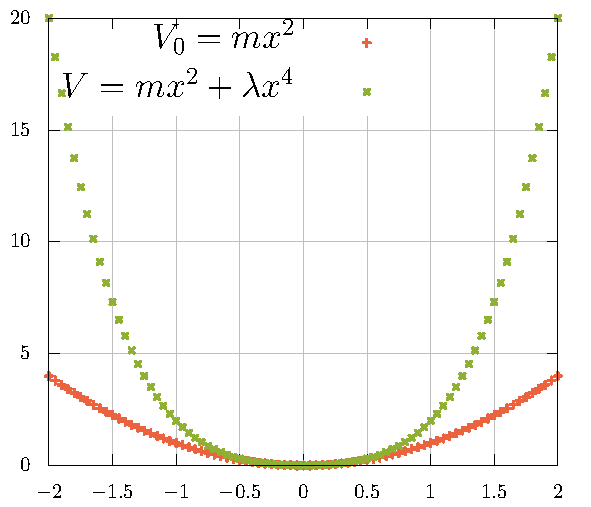
\includegraphics[width=69mm]{Graphs/anh1.pdf}}
  \subfigure{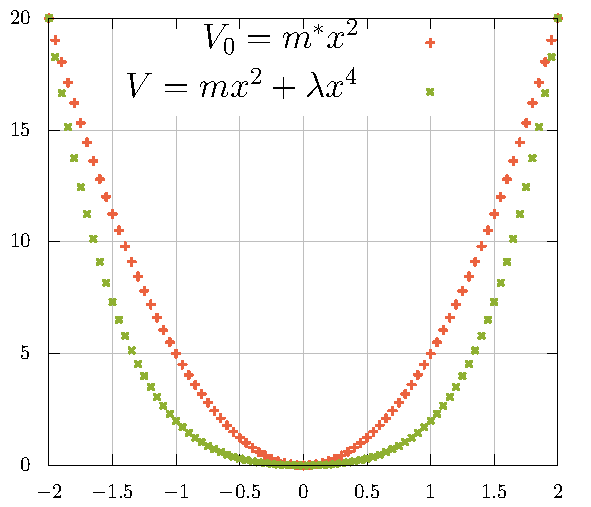
\includegraphics[width=69mm]{Graphs/anh2.pdf}}
  \caption{An illustrative one-dimensional example is the anharmonic oscillator, where effective mass can be introduced to align as closely as possible the unperturbed potential (a parabola) with the full potential (a quatric). 1-dimensional quatric potential approximated by the full quadratic part (left) and by the quadratic part with an effective parameter (right).}
  \label{EffParamFig}
\end{figure*}

The main idea of the ECM is to perform perturbative calculations of atomic properties in the basis of hydrogen-like functions, that is eigenvectors of the hydrogen-like Hamiltonian with the effective charge in place of the usual nuclear charge. Within the Schr\"odinger theory this means that our unperturbed Hamiltonian takes the form of
\begin{align}
\widehat{H}^0 (Z^*) = \sum_{i = 1}^{N} \widehat{H}^0_i(Z^*) = \sum_{i = 1}^{N}\left(-\frac{\widehat{p}_{i}^{2}}{2} - \frac{Z^*}{r_{i}}\right),
\end{align}
while the perturbation operator $\widehat{W}$ contains a single-electron and a two-electron parts that we will refer to as $\widehat{W}^{(1)}$ and $\widehat{W}^{(2)}$ respectively
\begin{equation} \label{Wdef}
\widehat{W} = \widehat{W}^{(1)} + \widehat{W}^{(2)} = \sum_{i=1}^{N} \frac{Z^*-Z}{r_i} +
\sum_{i<j}\frac{1}{|\vec{r}_i-\vec{r}_j|},
\end{equation}
where the indices $i,j$ run over the $N$ electrons.

As long as the value of effective charge is fixed, hydrogen-like wavefunctions form an orthonormal basis suitable for an expansion of the perturbation series. In the following we will refer to it as a hydrogen-like basis and index the hydrogen-like wavefunctions by a collective quantum number $\lambda$ that encompasses all four quantum numbers $(n,l,m,s)$, that specify a given eigenvector of the hydrogen equation in Schr\"odinger theory
\begin{align}
\widehat{H}^0_i |\lambda_i \rangle &= E_{\lambda_i}|\lambda_i \rangle, \\
\langle\vec r|\lambda \rangle &= \psi_{\lambda}(\vec{r}) = \psi_{n,l,m, Z^*}(\vec{r}).
\end{align}

For example, the ground state of
  the helium atom is given by $|\lambda_{1} \lambda_{2}\rangle$ with
  $\lambda_{1 }= 1s_{\uparrow}$ and $\lambda_{2} = 1s_{\downarrow}$.
  
Furthermore, as the initial approximation to the N-electron wavefunction, we take a Slater determinant of hydrogen like wavefunctions to ensure the anti-symmetry condition
\begin{equation} \label{effZdet}
  \langle\vec r_{1}\vec r_{2}\ldots\vec r_{N}|\lambda_1 \lambda_2 \dots \lambda_N \rangle = \frac{1}{\sqrt{N!}}
   \left| \begin{matrix} \psi_{\lambda_1}(\vec{r_1}) & \psi_{\lambda_2}(\vec{r_1}) & \dots & \psi_{\lambda_2}(\vec{r_1}) \\ 
    \vdots & & \ddots &  \\ 
    \psi_{\lambda_1}(\vec{r_N}) & \psi_{\lambda_2}(\vec{r_N})& \dots & \psi_{\lambda_N}(\vec{r_N})  \end{matrix} \right|,
\end{equation}
so that for example a two-electron wavefunction looks like
\begin{equation} \label{Exchange}
    |\lambda_{1} \lambda_{2}\rangle = \frac{|\lambda_{1} \rangle | \lambda_{2}\rangle-|\lambda_{2} \rangle | \lambda_{1}\rangle}{\sqrt{2}}.
\end{equation}
With this in mind, the Hamiltonian can be written in the secondary-quantized representation
\cite{feynman1972statistical}, as
\begin{align}
\widehat{H}^0 &= \sum_{\lambda}\langle\lambda|\widehat{H}^{\rm{kin}}-\frac{Z^{*}}{r}|\lambda\rangle a^{\dag}_{\lambda} a_{\lambda},\label{eq:5}
\\
\widehat{W}
&= \sum_{\lambda\lambda_{1}}\langle\lambda|\frac{-(Z -
	Z^{*})}{r}|\lambda_{1}\rangle  a^{\dag}_{\lambda}
a_{\lambda_{1}} +
\frac{1}{2}\sum_{\lambda\lambda_{1}\mu\mu_{1}}\langle\lambda|\langle\lambda_{1}|
\frac{1}{|\vec r - \vec r'|}|\mu_{1}\rangle|\mu\rangle 
a^{\dag}_{\lambda}  a^{\dag}_{\lambda_{1}}  a_{\mu} a_{\mu_{1}},\label{eq:6}
\end{align}
where $a_{\lambda}$ and $a^{\dag}_{\lambda}$ denote fermionic (so anticommuting) anihilation and creation operators, respectively, that create and destroy the state $|\lambda\rangle$.

An important property of the Schr\"odinger Hamiltonian~\eqref{SchH} is the charge-scale symmetry
\begin{equation}
    \widehat{H}^{\rm{Sch}}(\lambda Z, r/\lambda) = \lambda^2 \widehat{H}^{Sch}(Z,r).
\end{equation}
For this reason, all its eigenvalues and scale as $E_\lambda \sim (Z^*)^2$ and it's eigenvectors also have simple scalings with effective charge
\begin{align}
    E_{\lambda}(Z^*) &= (Z^*)^2E_{\lambda}(Z^*=1) \\
   \psi_{n,l,m,Z^*}(\vec{r}) &= (Z^*)^{3/2} \psi_{n,l,m,Z^*=1}(Z^* \vec{r}).
\end{align}
Importantly, this simple scaling carries over two multi-electron wavefunctions defined by~\eqref{effZdet}. This property will allow us to explicitly separate the dependence on effective charge in all subsequent calculations. It is one of the main reasons why the basis of hydrogen-like wavefunctions is particularly suited for deriving analytical approximations to atomic properties. 

\begin{figure} [t] 
	\centering
	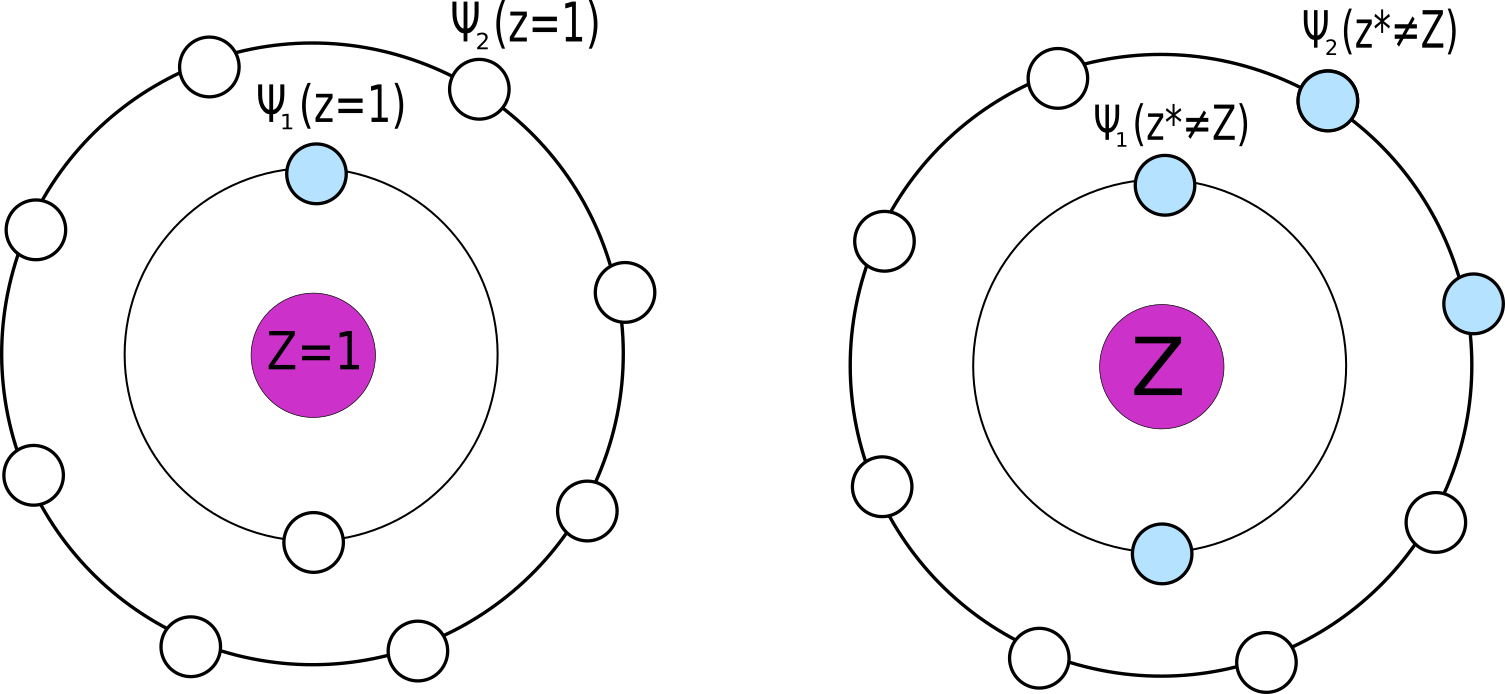
\includegraphics[width=119mm]{Graphs/ECM.png} 
	\caption{Pictorial representation of hydrogen wave functions with
		effective nuclear charge. Hydrogen atom on the left, as compared to an
		example of a multi-electron atom on the right. White circles represent virtual orbitals and coloured ones are filled.} \label{fol}
\end{figure}

  \section{Leading-order approximation}
  
We now have all the tools needed to calculate a perturbation series for the energy of a multi-electron atom. First step is to specify an electronic configuration described by $N$ collective quantum numbers $\lambda$. This defines an initial approximation of the eigenvector of the system as $|\lambda_{1}\ldots\lambda_{N}\rangle$. The initial approximation to the energy is meanwhile given by
\begin{equation}
E^0 = \langle \lambda_1 \lambda_2 ... \lambda_N | \widehat{H}_0 | \lambda_1
\lambda_2... \lambda_N \rangle = A Z^{*2},\label{eq:9}
\end{equation}
where $A$ is a sum of hydrogen energies of all single-electron
wave functions
\begin{equation}
A=\sum_i E_{\lambda_i} = \sum_i \frac{-1}{2n_i^2},\label{eq:8}
\end{equation}
and we have explicitly separated the dependence on effective charge.

The first order correction to the energy of the
system is given by an expectation value of $\widehat{W}$ (see.~\eqref{PertSeries})
\begin{equation} \label{FirstEnergy}
\Delta E^{(1)} = \langle \lambda_1 \lambda_2 ... \lambda_n |
\widehat{W}^{(1)}+\widehat{W}^{(2)} | \lambda_1 \lambda_2... \lambda_n \rangle =
\Delta E^{(1)}_{\rm{single}} + \Delta E^{(1)}_{\rm{double}}.
\end{equation}
The first term is a single sum over the residual nuclear interactions of all individual electrons
\begin{equation} \label{SchrA}
    \Delta E^{(1)}_{\rm{single}} = \sum_i \int \frac{|\psi_{\lambda_i}(r_i)|^2}{r_i} d\vec{r_i} = 2 Z^*(Z-Z^*)A,
\end{equation}
where we have separated the dependence on effective charge, by the change of variables $r \rightarrow r/Z^*$ and used~\eqref{Aformula}.

The second term in~\eqref{FirstEnergy} is a sum of the coulomb and exchange integrals
\begin{align} \label{FirstDouble}
\Delta E^{(1)}_{\rm{double}} &= \sum_{i<j} \langle \lambda_i \lambda_j|\frac{1}{|\vec{r}_i - \vec{r}_j|}|\lambda_i \lambda_j \rangle \nonumber\\
&= \sum_{i<j} \left(\langle \lambda_i| \langle \lambda_j|\frac{1}{|\vec{r}_i - \vec{r}_j|}|\lambda_i \rangle | \lambda_j \rangle  - \langle \lambda_i| \langle \lambda_j|\frac{1}{|\vec{r}_i - \vec{r}_j|}|\lambda_j \rangle | \lambda_i \rangle \right) \nonumber\\
 &= \sum_{i<j} \int \frac{|\psi_i(\vec{r}_i)|^2
	|\psi_j(\vec{r}_j)|^2 -
	\psi_i^*(\vec{r}_i)\psi_j^*(\vec{r}_i)\psi_i(\vec{r}_j)\psi_j(\vec{r}_j)}
{|\vec{r}_i - \vec{r}_j|} d \vec{r}_i d \vec{r}_j.
\end{align}
We can once again use the $r \rightarrow r/Z^*$ change of variables to explicitly separate the dependence on effective charge as
\begin{equation} \label{SchrB}
    \Delta E^{(1)}_{\rm{double}} = \sum_{i<j} (Z^* B^{Dir}_{\lambda_i,\lambda_j} - Z^* B^{Ex}_{\lambda_i,\lambda_j}) = B Z^*,
\end{equation}
where $B$ is now only dependent on the chosen configuration and not on $Z$ or $Z^*$. It can be calculated analytically
for any configuration, by employing the expansion of the electron-electron potential in spherical harmonics
\begin{equation} 
\frac{1}{|\vec{r}_i - \vec{r}_j|} = \sum_{l=0}^\infty \sum_{m=-l}^{l} \frac{4\pi}{2l+1}
\frac{\min[r,r']^l}{\max[r,r']^{l+1}} {Y_l^m}^*(\Omega)
Y_l^m(\Omega').
\end{equation}
We can then use \eqref{3jInt} to analytically calculate the angular integrals and obtain:
\begin{align}
    B^{Dir}_{\lambda_i,\lambda_j} = (-1)^{m_i+m_j}(2l_i+1)&(2l_j+1)\sum_{k=0}^{l_i+l_j}
    \begin{pmatrix} l_i & l_i & k \\ 0 & 0 & 0\end{pmatrix}
    \begin{pmatrix} l_j & l_j & k \\ 0 & 0 & 0 \end{pmatrix} \nonumber
\\& \times
    \begin{pmatrix} l_i & l_i & k \\ -m_i & m_i & 0 \end{pmatrix}
	\begin{pmatrix} l_j & l_j & k \\ -m_j & m_j & 0 \end{pmatrix} 
T^{\lambda_i,\lambda_j}_{\lambda_i,\lambda_j}(k),
\end{align}
\begin{align}
    B^{Ex}_{\lambda_i,\lambda_j} = (2l_i+1)(2l_j+1)\sum_{k=|l_i-l_j|}^{l_i+l_j}&
    \left| \begin{pmatrix} l_i & l_j & k \\ 0 & 0 & 0\end{pmatrix}\right|^2 \nonumber
\\& \times
    \left|\begin{pmatrix} l_i & l_j & k \\ -m_i & m_j & m_i-m_j \end{pmatrix}\right|^2
T^{\lambda_j,\lambda_i}_{\lambda_i,\lambda_j}(k),
\end{align}
where we have used the triangular conditions of the 3-$j$ symbols to restrict the sums (see Appendix~\ref{app:3j}). The general formula for the radial integral
\begin{equation}
    T^{\lambda_3,\lambda_4}_{\lambda_1,\lambda_2}(k) = \int R_{\lambda_1}(r_1) R_{\lambda_2}(r_2) R_{\lambda_3}(r_1) R_{\lambda_4}(r_2) \frac{\min[r_1,r_2]^k}{\max[r_1,r_2]^{k+1}} r_1^2 r_2^2 dr_1 dr_2,
\end{equation}
can also always be calculated analytically (see Appendix~\ref{app:ECM}).
Finally the sum of the zeroth- and first-order energies comes out as
\begin{equation} \label{Z-Z}
E^{(0)} + \Delta E^{(1)} = A Z^*(2Z-Z^*)+B Z^*.
\end{equation}
We have so far kept the value of effective charge arbitrary, since the perturbation series is valid for all possible values of $Z^*$. We are now in a position to make a choice of a specific value for the effective nuclear charge. In order to ensure the fastest convergence rate of the perturbation series, we fix it by
requiring the first-order correction to vanish
\begin{equation} \label{Z-Z}
\Delta E^{(1)} = 0 ~~\Rightarrow~~Z^* = Z - \frac{B}{2A} .
\end{equation}

Note that this also corresponds to the minimum of the energy calculated up to first-order
\begin{equation} \label{Z-Z}
\partial_{Z^*} (E^{(0)} + \Delta E^{(1)}) = 2A(Z-Z^*)+B,
\end{equation}
\begin{equation} \label{Z-Z}
\partial_{Z^*} (E^{(0)} + \Delta E^{(1)}) = 0 ~~\Rightarrow~~Z^* = Z + \frac{B}{2A} .
\end{equation}
For example, for helium-like ions, we have
\begin{equation}
    Z^* = Z-\frac{5}{16}.
\end{equation}

From now on we will refer to such setup, that is the zeroth-order plus the vanishing first-order, as the leading-order ECM. The values of effective charges for neutral atoms along with the corresponding leading-order energies are given in Appendix~\ref{app:GroundStates}.

We emphasize again that the value of effective charge is the same for all electrons of a given configuration, despite the intuitive picture where outer electrons are screened more than those closer to the nucleus. This is necessary in order to ensure orthonormality of the hydrogen-like basis.

Despite the simplicity of the above expressions, the zeroth-order calculation provides accuracy of the order of $\sim 5\%$ as compared to the HF calculation independently of the number of electrons (see Section~\ref{sec:ground-state-energ}). 

\section{Closed and open shells}

Since neither the Schr\"odinger nor the Dirac Hamiltonians depend on the projections of the angular orbital momentum, we do not expect any contributions to energy to depend on the magnetic quantum numbers $m$. Therefore we need to sum over the projections of each electrons angular momentum in all resulting formulas. We can do this in closed form using properties of the 3-$j$ symbols (see Appendix~\ref{app:3j}):
\begin{align} \label{3jProps}
    \sum_m (-1)^m\begin{pmatrix} l & l & k \\ -m & m & 0\end{pmatrix} = (-1)^l\delta_{k,0}\sqrt{2l+1}&,\\
    \sum_{m_1,m_2}
    \begin{pmatrix} l & l_1 & l_2 \\ m_1-m_2 & -m_1 & m_2 \end{pmatrix}
    \begin{pmatrix} k & l_1 & l_2 \\ m_2-m_1 & m_1 & -m_2 \end{pmatrix}
   & = \frac{\delta_{l,k}}{2l+1}.
\end{align}
For a closed shell (electrons with all $m_l$ present for a given $l$), we then get the $B$ values as:
\begin{align}
    B^{Dir}_{\lambda_i,\lambda_j} &= (2l_i+1)(2l_j+1) T^{\lambda_i,\lambda_j}_{\lambda_i,\lambda_j}(0),
\end{align}
\begin{align}
    B^{Ex}_{\lambda_i,\lambda_j} &= \sum_{k=|l_i-l_j|}^{l_i+l_j}
    \left| \begin{pmatrix} l_i & l_j & k \\ 0 & 0 & 0\end{pmatrix}\right|^2
T^{\lambda_j,\lambda_i}_{\lambda_i,\lambda_j}(k).
\end{align}

For open shells the situation is more complicated. In order to describe an open shell correctly, we need to use a linear combination of many basis state configurations. In general, this requires a diagonalization of the total Hamiltonian in the basis of the configurations comprising a given open shell. In many instances this can be replaced by assuming a particular coupling (more details in Section~\ref{sec:Coupling}).

\section{Relativistic effective charge model}

In order to derive the D-ECM within the Dirac theory, we proceed in exactly the same way as above, but starting from the Dirac Hamiltonian with the effective charge $Z^*$
\begin{align} \label{DiracH}
H^0 = \sum_{i = 1}^{N} H^0_i = \sum_{i = 1}^{N}\left(\vec{\alpha} \cdot \vec{\nabla_i} + \alpha_0 c  - \frac{Z^*}{r_i}\right),
\end{align}
with the same perturbation operator $W$ given by~\eqref{Wdef}.

The eigenvectors of~\eqref{DiracH} are the hydrogen-like Dirac wavefunctions given by~\eqref{Diracwave} but with effective charge $Z^*$ in place of the nuclear charge $Z$. As long as the value of effective charge is fixed, they form an orthonormal basis in which we can perform a perturbation calculation. In order to compute the energy of the system we specify a set of $N$ collective
quantum numbers $\lambda_{1}, \ldots, \lambda_{N}$, which
characterizes the state of $N$ electrons
$|\lambda_{1},\ldots,\lambda_{N}\rangle$ given by a Slater determinant of single-electron wavefunctions~\eqref{effZdet}. 

In analogy to the non-relativistic case, the zeroth-order energy $E^{(0)}(Z^{*})$
is a sum of hydrogen-like Dirac energies over the occupied states
\begin{align}
  E^{(0)}(Z^{*}) = \sum_{{\lambda_{i}} = (n_{r}\kappa m_{j})_{i}}
  E_{\lambda_i}(Z^{*}). \label{eq:9} 
\end{align}
Notice that now $\lambda$ refers to a collection of relativistic quantum numbers, specifying a hydrogen-like wavefunction within the Dirac theory.

Evaluation of the first-order correction to the energy of the
system is also straightforward
\begin{equation}
    \Delta E^{(1)}_{\rm{single}} = \sum_i \int \frac{|\psi_{\lambda_i}(r_i)|^2}{r_i} d\vec{r_i} = \sum_i Z^*(Z-Z^*)T_{\lambda_i},
\end{equation}
with the analytic result for individual $T_{\lambda}$ coefficients given by (see Appendix~\ref{app:ECM})
\begin{equation} \label{DiracA}
    T_{\lambda} = \left(\frac{(\alpha Z^*)^2}{\gamma}+n_k\right)\left(\frac{\varepsilon}{n_k}\right),
\end{equation}
where $n_k$ and $\gamma$ are defined as in~\eqref{nkdef} and $\alpha$ is the fine-structure constant.

The double-electron first order correction is still given by the sum of Coulomb and exchange integrals~\eqref{FirstDouble}, but now both angular and radial parts contain contributions from all four components of the wavefunction, making the resulting formulas more complicated. Nevertheless, we can use the Wigner-Eckhart theorem~\cite{sakurai2020modern} along with~\eqref{3jProps} to find that for a closed shell the results read:
\begin{equation}
    B^{Dir}_{\lambda_1,\lambda_2} = 4 |\kappa_1 \kappa_2| T_{\lambda_1,\lambda_2}^{\lambda_1,\lambda_2},
\end{equation}
\begin{align}
    B^{Ex}_{\lambda_1,\lambda_2} &= \sum_{p=|l_1-l_2|}^{l_1+l_2}(\kappa_1+\kappa_2+p+1)(\kappa_1+\kappa_2-p) %\\  &\times 
    \left| \begin{pmatrix} l_1 & l_2 & p \\ 0 & 0 & 0\end{pmatrix}\right|^2 T_{\lambda_1,\lambda_2}^{\lambda_2,\lambda_1}(p),
\end{align}
where the radial integrals are now given by
\begin{equation}
  T_{\lambda_1,\lambda_2}^{\lambda_3,\lambda_4} (k) = \int R_{\lambda_1,\lambda_2}(r_1,r_2)\frac{\min[r_1,r_2]^k}{\max[r_1,r_2]^{k+1}}R_{\lambda_3,\lambda_4}(r_1,r_2)r_1^2 r_2^2 dr_1 dr_2,
\end{equation}
and we have written
\begin{equation}
    R_{\lambda_1,\lambda_2}(r_1,r_2) = g_{\lambda_1}(r_1)^*g_{\lambda_2}(r_2)+f_{\lambda_1}(r_1)^*f_{\lambda_2}(r_2).
\end{equation}
%In addition, we mention here that fermionic operators of negative
%energies do not contribute to the energy of the system in the zeroth-
%and first-order as we are considering the corrections only to the
%electronic states, that is the states that do not contain $\mu_{i}$
%quantum numbers. However, starting from second-order
%perturbation theory, the negative energy states will contribute to the
%observable characteristics, since there exist nonvanishing matrix
%elements due to the structure of the interaction operator $\widehat{W}$.

To find the effective charge we proceed in analogy with
the non-relativistic case and choose it from the condition
that the first-order correction to the energy of the system for a
given state is vanishing, i.e.
\begin{align}
  \Delta E^{(1)}(Z^*, Z, N) = 0. \label{eq:13}
\end{align}
For this reason the expression for the energy of the system in
the leading order is given via a sum of hydrogen-like
energies, Eq.~(\ref{eq:9}) with the effective charge $Z^{*}$, defined
as a solution of Eq.~(\ref{eq:13}).

It is worth noting here, that the nontrivial dependence of Dirac
hydrogen wave functions on the nuclear charge makes it impossible to
separate the effective charge from the above integrals. This means
that contrary to the nonrelativistic case, $A_{\lambda_{k}}$ and
$B^{\lambda_{1},\lambda_{3}}_{\lambda_{2},\lambda_{4}}$ are implicitly
dependent on $Z^*$. This is related to the fact, that the Dirac
equation, unlike the Schr\"{o}dinger equation, is not scale
invariant. In fact, rescaling the radial variable $r$ in a
Schr\"{o}dinger hydrogen atom effectively changes its charge, while
in the Dirac hydrogen atom effectively changes both the mass of the electron and the nuclear charge. 

For this reason, solving Eq.~(\ref{eq:13}) for $Z^*$ means finding a root of a transcendental equation containing
gamma functions. For example, the relativistic effective charge $Z^*$
of a helium-like atom or ion with nuclear charge $Z$ is found by
solving
\begin{equation}
  2(Z^*-Z)+1 = \frac{\Gamma(2\gamma+1/2)}{\Gamma(2\gamma+1)\sqrt{\pi}},
\end{equation}
where $\gamma = \sqrt{1-(\alpha Z^*)^2}$. Such equation can be solved
to any desired accuracy with traditional iterative methods from
numerical analysis or with analytical approximations. In the latter
case, the Taylor series of the gamma function can be used to
approximate the effective charge to any order in $\alpha$. Up to the
second order in $\alpha$ it reads
\begin{equation*}
  Z^* = Z-\frac{5}{16}+\alpha^2 \left(Z-\frac{5}{16}\right)^2
  \frac{12 \log(2)-7}{32}+O[\alpha^4].
\end{equation*}
%
Analogously, similar expressions can be written for any 
	other atom or ion. Values of effective charges for neutral atoms along with the corresponding leading-order energies are given in the Appendix~\ref{app:ECM}.



\chapter{Second-order effective charge model}
\addtocontents{toc}{\contentsline{chapter}{Second-order effective charge model}{\protect\pageref{annotation}}}
\label{ch:secondECM}

This chapter explains how to use the Green's function of the hydrogen equation to calculate second-order corrections to energies in the ECM. This includes corrections coming from adjusting the shapes of single-electron orbitals, as well as from electron-electron correlations. It also shows how to mitigate the divergences coming from the degeneracy of the hydrogen-like basis. Just like in the leading-order we avoid making any approximations beyond limiting the discussion to the second order of perturbation.

\section{Green's functions}
\label{sec:Green}

Second order correction to energy is given by the sum over all virtual multi-particle virtual states $\psi_k$
\begin{equation}
    \Delta E^{(2)} = \sum_k \frac{|\langle \psi^{(0)}|\widehat{W}|\psi_k\rangle|^2}{E^{(0)}-E_k}
\end{equation}
where the sum runs over all discrete and continuous states in the hydrogen-like basis  (see~\eqref{PertSeries}).

Since $W$ is a two-electron operator, only virtual states that differ by at most two single-electron orbitals contribute to the above sum. Hence for $|\psi^{0}\rangle = |\lambda_1...\lambda_n\rangle$, we have
\begin{equation} \label{SecondSigma}
    \Delta E^{(2)} = \sum_{k \neq l}^n \left(\sum_{\sigma} \frac{|\langle \lambda_k \lambda_l|\widehat{W}|\lambda_k \sigma \rangle|^2}{E_{\lambda_l}-E_\sigma} + \sum_{\sigma,\sigma'}\frac{|\langle \lambda_k \lambda_l|\widehat{W}|\sigma \sigma' \rangle|^2}{E_{\lambda_k}+E_{\lambda_l}-E_\sigma-E_{\sigma'}}\right)
\end{equation}
where $\sigma$ denotes the single-electron virtual states of the hydrogen-like basis.

We will refer to the first of these two terms as the single-electron second-order correction, denoted $\Delta E^{(2)}_{\rm{single}}$ and to the second as the double-electron second-order correction, denoted $\Delta E^{(2)}_{\rm{double}}$. Physically, the single-electron correction represents the adjustment of the shapes of single-electron orbitals, while the double-electron correction is related to the correlations between electrons.

At a first glance these corrections may seem complicated, but all of the above sums can be expressed in terms of the Green's function \footnote{This is a slight abuse of notation, as the sum includes all discrete and continuous spectra of the given basis. For example, in the case of hydrogen wavefunctions, we can write more explicitly $G_E = \sum_{n=1}^{\infty} \frac{|\psi_n \rangle\langle \psi_n|}{E-E_n} + \int \frac{|\psi_p \rangle\langle \psi_p|}{E-E_p} dp$.}
\begin{equation} \label{spectralG}
	G_E = \sum_{k} \frac{|\psi_k \rangle\langle \psi_k|}{E-E_k},
\end{equation}
which in practice can often be found for a basis generated by $H_0$ by using the Laplace transform~\cite{Swainson_1991} to solve the difing equation
\begin{equation}
	(H^0 - E^0)G_{E^0} = \delta.
\end{equation}
In the particular case of the non-relativistic hydrogen basis the Green's function is known analytically and can be written as~\cite{friedman1990principles}
\begin{align} \label{GreenESch}
G_E(r,r')
&=  \sum_{l=0}^\infty \sum_{m=-l}^{l} G_{l,E} (r,r')
Y_{l,m}^*(\Omega) Y_{l,m}(\Omega'), \nonumber
\\
G_{l,E} (r,r') &=\frac{(-1)^{1-l-\nu} \nu^3 \pi}{Z^2 \sin((\nu-l)\pi)}
R_{\nu,l}\left(Z r_{<}\right) U_{\nu,l}\left(Z r_{>}\right),
\end{align}
where $\nu = Z/\sqrt{-2E}$, while $R$ and $U$ are the two solutions of the Schr\"odinger radial hydrogen equation (see Appendix~\ref{app:hydrogen} for details).

In the relativistic case meanwhile, the Green's function of the hydrogen basis is given, by
\begin{align} \label{GreenEDirac}
G_E(r,r')
&=   \sum_{\kappa,m} G_{\kappa,E} (r,r') \left(\begin{matrix} \Omega_{\kappa,m}(\Omega) \\ \Omega_{-\kappa,m}(\Omega)\end{matrix}\right)^\dag \otimes \left(\begin{matrix} \Omega_{\kappa,m}(\Omega') \\ \Omega_{-\kappa,m}(\Omega')\end{matrix}\right),\nonumber
\\
G_{\kappa,E} (r,r') &=\frac{(-1)^{|\kappa|-\nu} Z \pi}{\omega^3 \sin((|\kappa|-\nu)\pi)}
\Big(\theta(r'-r)R_{\nu,\kappa,Z}(r)^\dag \otimes U_{\nu,\kappa,Z}(r') \nonumber
\\
&\hspace{50mm}+\theta(r-r')U_{\nu,\kappa,Z}(r)^\dag \otimes R_{\nu,\kappa,Z}(r')\Big),
\end{align}
where $\nu$ is the solution of $E=E^{\rm{Dirac}}_{\nu,\kappa}$ defined by~\eqref{DiracEnergy}, while $R$ and $U$ are the two solutions of the Dirac radial hydrogen equation (see Appendix~\ref{app:hydrogen} for details). Notice that combining the two 4-component spinors with an outer product $\oteimes$ means that the Dirac hydrogen Green's function is a $4\times4$ matrix.

\section{Reduced Green's functions}

It is clear from both the spectral representation~\eqref{spectralG}, as well as the explicit formulas~\eqref{GreenESch} and~\eqref{GreenEDirac}, that the Green's functions have poles at the values of energy corresponding to the bound states. For this reason, we cannot directly use them to evaluate the second-order energy corrections. In fact, we need the reduced Green's function defined as the limit
\begin{equation} \label{Glimit}
	\widetilde G_n = \lim_{\delta \rightarrow 0} G_{E_n+i \delta} - \frac{|\psi_n \rangle \langle \psi_n|}{i \delta}.
\end{equation}
We will subsequently denote the reduced Green's functions with an overhead tilde $\widetilde{G}$ in order to distinguish from full Green's functions $G$. The explicit form of the reduced Schr\"odinger (RCGF) and Dirac (RCDGF) Green's functions is discussed in chapter~\ref{ch:IntGreen}.

In terms of the reduced Green's function, the corrections to energies and wavefunctions in a general perturbation series read
\begin{align}
	\Delta E^{(2)}_{\rm{single}} &= \langle \psi^0_n|\widehat{W}\widetilde G_{E_n} \widehat{W}|\psi^0_n\rangle,
	\\
	\Delta|\psi_n^{(1)}\rangle &= \widetilde G_{E_n} \widehat{W}|\psi^0_n\rangle,
\end{align}
and we can use the hydrogen Green's function in particular to write the single-electron second-order correction, as
\begin{equation} \label{SecondSingle}
    \Delta E^{(2)}_{\rm{single}} = \sum_{m,k,l} \langle \lambda_k \lambda_l|\widehat{W} |\lambda_k \widetilde{G}_{\lambda_l} \lambda_m|\widehat{W}|\lambda_l \lambda_m \rangle.
\end{equation}

	\begin{figure}
			\centering
			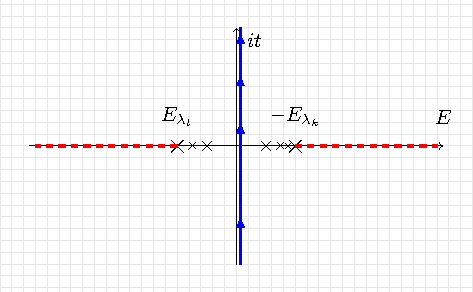
\includegraphics[width=120mm]{Graphs/Contour.pdf} 
			\caption{Diagram of the integration contour used in~\eqref{contour}. Crosses represent poles corresponding to bound states, while red dashed lines represent branch cuts corresponding to the continuous spectrum of free states. There are no poles at $t=0$, as the $\lambda_k$ and $\lambda_l$ states are omitted in the spectral representations of the corresponding reduced Green's functions} \label{degeneracyFig}
		\end{figure}
	
In order to express the double-electron correction however, we need the two-electron reduced hydrogen Green's function with spectral representation of
\begin{equation}
\widetilde{G}_{\lambda_k,\lambda_l}^2 = \sum_{\substack{\sigma_1 \neq \lambda_k\\\sigma_2 \neq \lambda_l}} \frac{|\sigma_1\rangle |\sigma_2\rangle \langle
	\sigma_1| \langle \sigma_2|}{E_{\lambda_k} + E_{\lambda_l} -
	E_{\sigma_1} - E_{\sigma_2}}.\label{eq:16}
\end{equation}
Unfortunately, it does not have a closed form, but borrowing a clever trick from complex analysis we can express it as a convolution over the energy of two single-electron Green's functions
\begin{equation}
\widetilde{G}^{(2)}_{\lambda_k,\lambda_l} (r_1,r_2,r_3,r_4) = \int
\widetilde{G}_{E_{\lambda_k}+it}(r_1,r_2)\widetilde{G}_{E_{\lambda_l}-it}(r_3,r_4)
\frac{dt}{2 \pi i}\label{contour} .
\end{equation}
This somewhat surprising formula follows immediately from applying the
following identity, which is simply a residue theorem for a product of
simple poles, directly to the above spectral representation of the Green's function
\begin{equation}
\int \frac{1}{a+it}\frac{1}{b-it}dt = \frac{-2 \pi}{a+b},\label{eq:18}
\end{equation}
which is valid, provided that both $a$ and $b$ are negative,
which will always be the case in the ground state, as they stand for
differences between the ground state energy and intermediate energies.

With that in mind, the single-electron second order correction can simply be calculated, as
\begin{equation}\label{SecondDouble}
    \Delta E^{(2)}_{\rm{double}} = \sum_{k \neq l} \langle \lambda_k \lambda_l|\widehat{W} \widetilde{G}^{(2)}_{\lambda_k,\lambda_l} \widehat{W}|\lambda_k \lambda_l \rangle,
\end{equation}
where exchange elements are implied according to~\eqref{Exchange}.

\section{Subtractions}

At this point, we still need to take into account the Pauli exclusion principle. It manifests itself in the fact that sums over $\sigma$ in~\eqref{SecondSigma}, do not include occupied single-electron orbitals. This means that despite using reduced Greens functions we still need to subtract all other occupied states.

This means subtracting the following sum from the single-electron second order correction
\begin{equation}
  \sum_{m \neq k \neq l} \frac{|\langle \lambda_k \lambda_l|\widehat{W} |\lambda_k \lambda_m\rangle |^2}{E_{\lambda_l} - E_{\lambda_m}}.
\end{equation}
 And from the double-electron one
\begin{equation}
  \sum_{n \neq m,k \neq l} \frac{|\langle \lambda_k \lambda_l|\widehat{W} |\lambda_m \lambda_n\rangle |^2}{E_{\lambda_l}+E_{\lambda_k} - E_{\lambda_m} - E_{\lambda_n}}.
\end{equation}

However note that all terms in the above sums are anti-symmetric with respect to the $l \rightarrow m$ and $(k,l) \rightarrow (m,n)$ exchanges respectively, so the total amount subtracted from the correction to any multi-electron configuration is equal to zero. This can also serve as a useful check of the consistency of all calculations.

\section{Effects of degeneracy}

Naive application of the above formulas will lead to divergent results for many electronic configurations, even including some of the ground states of neutral atoms. This is because of the high degeneracy of the hydrogen-like basis, in particular the lack of energy dependence on the angular momentum quantum number. It can be readily seen from the formula for the reduced Greens function used in the derivation of the second order energy corrections
\begin{equation}
    G^{\psi_0}=\sum_k\frac{|\psi_k\rangle\langle\psi_k|}{E_{\psi_0}-E_{\psi_k}}.
\end{equation}

This leads to a divergence whenever for any of the virtual states $\psi_k$ we have $E_{\psi_k} = E_{\psi_0}$. It is never the case when calculating single-electron corrections as there are no elements $\langle \psi_k|\widehat{W}|\psi_l\rangle$ with non-zero amplitudes, that change the angular momentum quantum number of exactly one electron. However, it does happen when calculating the double electron correction, for example to the ground state of beryllium, as $\langle 2s 2s|\widehat{W}|2p2p\rangle \neq 0$ (see Figure~\ref{degeneracyFig}).

	\begin{figure}
			\centering
			\includegraphics[width=120mm]{Graphs/degeneracy.png} 
			\caption{Pictorial representation of an example of an intermediate state
				with degenerate energy, causing a divergence in
				the double-electron second order correction to the energy of beryllium. Such transitions do not happen in elements that have at least half-filled outer shells or only a single valance electron e.g. lithium.} \label{degeneracyFig}
		\end{figure}
	
	In order to mitigate this, whenever there are multiple configurations with equal zeroth-order energy, we have to diagonalize the Hamiltonian in the subspace spanned by those configurations and consider it's eigenvectors as the new zeroth-order approximations. On top of regularizing divergences, this further increases the accuracy of the ECM calculation as it effectively includes corrections of all orders coming from those configurations. The resulting zeroth-order wavefunction is then a linear combination of those degenerate configurations. For example the ground state configuration of berylium becomes\footnote{We show approximate coefficients for clarity, but they can be calculated as exact analytical numbers within the ECM.} $0.9743|1s^22s^2\rangle + 0.2252|1s^22p^2\rangle$.
	
	This means that we have more contributions to the second-order correction in such cases, as now transitions to all virtual states that differ by no more than two electrons from any of the zeroth order degenerate basis states have to be taken into account.  It is important to note, that all of those configurations differ by exactly two electrons (for reasons mentioned above). So for a wavenuction
	\begin{equation}
    |\psi\rangle = \sum_i \alpha_i |\lambda^i_1...\lambda^i_n \rangle = \sum_i \alpha_i |\lambda_1...\lambda_{n-2} \chi_1^i \chi_2^i \rangle,
\end{equation}
we get the correction
\begin{align}
    \Delta E^{(2)}_{\rm{single}} =& \sum_{m \neq l \neq k}^{n} \sum_i\alpha_i^2 \langle \lambda^i_k \lambda^i_l|\widehat{W} |\lambda^i_k \widetilde{G}_{\lambda^i_l} \lambda^i_m|\widehat{W}|\lambda^i_l \lambda^i_m \rangle \nonumber 
    \\
    &+\sum_{i,j}\sum_{k} \alpha_i \alpha_j\langle \lambda_k \chi^i_1|\widehat{W} |\lambda_k \widetilde{G}_{\lambda} \chi^i_2|\widehat{W}|\chi^j_1 \chi^j_2 \rangle \nonumber
    \\
    & + \sum_{i,j}\sum_{k} \alpha_i \alpha_j\langle \lambda_k \chi^i_1|\widehat{W} |\chi^j_1 \widetilde{G}_{\lambda} \chi^i_2|\widehat{W}|\chi^j_2 \lambda_k \rangle \nonumber 
    \\
    &+ \sum_{i,j}\sum_{k \neq l} \alpha_i \alpha_j \frac{\langle \lambda_k \lambda_l|\widehat{W} |\chi^i_1\chi^i_2 \rangle\langle \lambda_k \lambda_l |\widehat{W}|\chi^j_1 \chi^j_2 \rangle}{E_k+E_l-2E_{\chi}}.
\end{align}
Similarly, the double electron correction becomes
\begin{align}
    \Delta E^{(2)}_{\rm{double}} =& \sum_i \sum_{k \neq l} \alpha_i^2 \langle \lambda^i_k \lambda^i_l|\widehat{W} \widetilde{G}^{(2)}_{\lambda^i_k,\lambda^i_l} \widehat{W}|\lambda^i_k \lambda^i_l \rangle \nonumber \\
    &+ \sum_{i \neq j}  \alpha_i \alpha_j \langle \chi^i_1 \chi^i_2|\widehat{W} \widetilde{G}^{(2)}_{\chi^i_1,\chi^i_2} \widehat{W}|\chi^j_1 \chi_j^2 \rangle,
\end{align}
where the subtractions in all Greens functions now include all states contained in any of the degenerate configurations.


\section{Closed subshells}

Finally we want to show closed form formulas for the summation over projections of angular momenta. Using the generalized orthogonality relation of 3-$j$ symbols~\cite{cowan1981theory}
\begin{align} \label{3jProps2}
    \sum_m (-1)^m\begin{pmatrix} l & l & k \\ -m & m & 0\end{pmatrix} = (-1)^l\delta_{k,0}\sqrt{2l+1}&, \\
    \sum_{m_1,m_2}
    \begin{pmatrix} l & l_1 & l_2 \\ m_1-m_2 & -m_1 & m_2 \end{pmatrix}
    \begin{pmatrix} k & l_1 & l_2 \\ m_2-m_1 & m_1 & -m_2 \end{pmatrix}
    &= \frac{\delta_{l,k}}{2l+1},
\end{align}
we can immediately obtain the formula for the direct term of the single-electron second-order correction:
\begin{align}
    \sum_{m_k,m_l,m_m}\langle \lambda_k |\langle\lambda_l|\widehat{W} |\lambda_k \widetilde{G}_{\lambda_l} &\lambda_m|\widehat{W}|\lambda_l \rangle |\lambda_m \rangle \nonumber \\
    &= (2l_k+1)(2l_m+1)(2l_l+1)I^{\lambda_k,\lambda_l,\lambda_k,\lambda_m,\lambda_l,\lambda_m}_{l_l,0,0},
\end{align}
and the two distinct exchange terms:
\begin{align}
    \sum_{m_k,m_l,m_m}&\langle \lambda_l |\langle\lambda_k|\widehat{W} |\lambda_k \widetilde{G}_{\lambda_l} \lambda_m|\widehat{W}|\lambda_l \rangle |\lambda_m \rangle \nonumber
    \\
    &=\sum_p(2l_k+1)(2l_m+1)(2l_l+1)
    \times\begin{pmatrix} l_k & l_l & p \\ 0 & 0 & 0 \end{pmatrix}^2I^{\lambda_l,\lambda_k,\lambda_k,\lambda_m,\lambda_l,\lambda_m}_{l_l,p,0},
\end{align}
\begin{align}
    \sum_{m_k,m_l,m_m}&\langle \lambda_l |\langle\lambda_k|\widehat{W} |\lambda_k \widetilde{G}_{\lambda_l} \lambda_m|\widehat{W}|\lambda_m \rangle |\lambda_l \rangle \nonumber 
    \\
    &= \sum_{p_1,p_2}(2l_k+1)(2l_m+1)\begin{pmatrix} l_k & l_l & p_1 \\ 0 & 0 & 0 \end{pmatrix}^2\begin{pmatrix} l_m & l_l & p_2 \\ 0 & 0 & 0 \end{pmatrix}^2I^{\lambda_l,\lambda_k,\lambda_k,\lambda_m,\lambda_l,\lambda_m}_{l_l,p_1,p_2},
\end{align}
where the radial integrals are of the form
\begin{align}
    I^{\lambda1,\lambda2,\lambda3,\lambda4,\lambda5,\lambda6}_{p,k,k'} = \int R_{\lambda2}(r)R_{\lambda5}(r')W^k_{\lambda1,\lambda3}(r)W^{k'}_{\lambda4,\lambda6}(r') G_{\lambda_2,p}(r,r')dr dr',
\end{align}
with the potential generated by the electron-electron repulsion defined as
\begin{equation}
    W^k_{\lambda1,\lambda2}(r) = \int R_{\lambda1}(r')R_{\lambda2}(r') \frac{\min[r,r']^k}{\max[r,r']^{k+1}}dr'.
\end{equation}

The analogous calculation for the double-electron contribution is only slightly more involved. Lets first consider an exchange energy between two subshells. For closed subshells $\lambda \neq \lambda'$
\begin{equation}
    \Delta E^{(2)}_{\rm{double}} = \sum_{m,m'}(\langle \lambda \langle \lambda'|\widehat{W} GG \widehat{W}|\lambda \rangle \lambda'\rangle-\delta_{s,s'}\langle \lambda \langle \lambda'|\widehat{W} GG \widehat{W}|\lambda' \rangle \lambda \rangle),
\end{equation}
where the Kronecker delta is 1 if the spins are aligned and 0 otherwise, and we have explicitly expanded the exchange symmetry.

For the case of $\lambda=\lambda'$ we have
\begin{align}
    \Delta E^{(2)}_{\rm{double}} &= \sum_{m>m'}(\langle \lambda_m \lambda_{m'}|\widehat{W} GG \widehat{W}|\lambda_m \lambda_{m'}\rangle-\langle \lambda_{m} \lambda_{m'}|\widehat{W} GG \widehat{W}|\lambda_{m'} \lambda_{m} \rangle) \nonumber\\
    &= \frac{1}{2} \sum_{m,m'}(\langle \lambda_m \lambda_{m'}|\widehat{W} GG \widehat{W}|\lambda_m \lambda_{m'}\rangle-\langle \lambda_{m} \lambda_{m'}|\widehat{W} GG \widehat{W}|\lambda_{m'} \lambda_{m} \rangle).
\end{align}
where we have used the $m \leftrightarrow m'$ symmetry and the fact that the case $m=m'$ cancels out. Therefore we can see that the only difference between those cases is the factor of $1/2$, wchich is related to the exchange antisymmetry of single-electron states.

Using~\eqref{3jProps2} we get the sum over projections in the direct term as
\begin{align}
    &\sum_{m,m'}\langle \lambda \lambda'|\widehat{W} GG \widehat{W}|\lambda \lambda'\rangle \nonumber \\
    &= \sum_{p,q,k} \frac{(2l+1)(2l'+1)(2p+1)(2q+1)}{(2k+1)^2}\left(\begin{matrix}l&p&k\\0&0&0\end{matrix}\right)^2\left(\begin{matrix}l'&q&k\\0&0&0\end{matrix}\right)^2I^{\lambda,\lambda',\lambda,\lambda'}_{p,q,k,k},
\end{align}
where the radial integrals are of the form
\begin{align}
    I^{\lambda1,\lambda2,\lambda3,\lambda4}_{p,q,k,k'} =& \int R_{\lambda1}(r_1)R_{\lambda2}(r_2)R_{\lambda3}(r_3)R_{\lambda4}(r_4) G^{\lambda}_{p,t}(r_1,r_3)G^{\lambda'}_{q,-t}(r_2,r_4) \nonumber\\
    &\times \frac{\min[r_1,r_2]^k}{\max[r_1,r_2]^{k+1}}\frac{\min[r_3,r_4]^{k'}}{\max[r_3,r_4]^{k'+1}}dr_1dr_2dr_3dr_4dt.
\end{align}

 Similarly, we can sum over projections in the calculation of the exchange element, using the definition of the 6-$j$ symbol~\cite{cowan1981theory}
\begin{align}
   \sum_{m_1...m_6}(-1)^\xi&\left(\begin{matrix}j_1&j_2&j_3\\-m_1&-m_2&-m_3\end{matrix}\right)\left(\begin{matrix}j_1&j_5&j_6\\m_1&-m_5&m_6\end{matrix}\right) \nonumber\\
   &\times\left(\begin{matrix}j_4&j_2&j_6\\m_4&m_2&-m_6\end{matrix}\right)\left(\begin{matrix}j_4&j_5&j_3\\-m_4&m_5&m_3\end{matrix}\right) =  \bigg\{\begin{matrix}j_1&j_2&j_3\\j_4&j_5&j_6\end{matrix}\bigg\},
\end{align}
where $\xi = \sum_i (j_i-m_i)$. The final expression comes out as
\begin{align}
    \sum_{m,m'}\langle \lambda \lambda'|\widehat{W} GG \widehat{W}|\lambda' \lambda\rangle =& \sum_{p,q,k,k'} (2l+1)(2l'+1)(2p+1)(2q+1) \nonumber\\
    &\times\left(\begin{matrix}l&p&k\\0&0&0\end{matrix}\right)\left(\begin{matrix}l&q&k'\\0&0&0\end{matrix}\right)\left(\begin{matrix}l'&p&k'\\0&0&0\end{matrix}\right) \nonumber
    \\
    &\times\left(\begin{matrix}l'&q&k\\0&0&0\end{matrix}\right)\bigg\{\begin{matrix}l&p&k\\l'&q&k'\end{matrix}\bigg\}I^{\lambda,\lambda',\lambda',\lambda}_{p,q,k,k'}.
\end{align}

Since the resulting formulas are somewhat involved, it is instructive to look at the first few examples. For the case of $\lambda\neq\lambda'$ we get the correlations between the $s$ and $p$ shells:
\begin{align}
    \lambda_s,\lambda'_s &: \Delta E^{(2)}_{\rm{double}}= \sum_a \frac{2a+1}{16 \pi^2} (I^{\lambda,\lambda',\lambda,\lambda'}_{a,a,a,a} - I^{\lambda,\lambda',\lambda',\lambda}_{a,a,a,a}) \\
    \lambda_s,\lambda'_p &:\Delta E^{(2)}_{\rm{double}}= \sum_a \frac{3(a+1)}{16 \pi^2} (I^{\lambda,\lambda',\lambda,\lambda'}_{a,a+1,a,a}+I^{\lambda,\lambda',\lambda,\lambda'}_{a+1,a,a,a} \\
    &+ I^{\lambda,\lambda',\lambda,\lambda'}_{a+1,a,a+1,a+1}+I^{\lambda,\lambda',\lambda,\lambda'}_{a,a+1,a+1,a+1}-I^{\lambda,\lambda',\lambda',\lambda}_{a+1,a,a+1,a}-I^{\lambda,\lambda',\lambda',\lambda}_{a,a+1,a,a+1}) \\
  \lambda_p,\lambda'_p &:\Delta E^{(2)}_{\rm{double}}= \frac{9}{16\pi^2}\sum_a [\frac{(a+1)^2}{(2a+1)}I^{\lambda,\lambda',\lambda,\lambda'}_{a+1,a+1,a,a} +\frac{(a+1)^2}{(2a+3)}I^{\lambda,\lambda',\lambda,\lambda'}_{a,a,a+1,a+1} \\
  &-\frac{a+1}{(2a+1)(2a+3)}(I^{\lambda,\lambda',\lambda',\lambda}_{a+1,a+1,a,a} +I^{\lambda,\lambda',\lambda',\lambda}_{a,a,a+1,a+1}) \\
 &+2 \frac{(a+1)(a+2)}{(2a+3)}(I^{\lambda,\lambda',\lambda,\lambda'}_{a,a+2,a+1,a+1}-I^{\lambda,\lambda',\lambda',\lambda}_{a+1,a+1,a,a+2} -I^{\lambda,\lambda',\lambda',\lambda}_{a,a+2,a+1,a+1})]
\end{align}
where the exchange parts should be skipped if $\lambda$ and $\lambda'$ have opposite spins.

On the other hand when $\lambda=\lambda'$ the same terms read:
\begin{align}
    \lambda_s,\lambda_s &: \Delta E^{(2)}_{\rm{double}}= 0 \\
  \lambda_p,\lambda_p &: \Delta E^{(2)}_{\rm{double}}= \frac{9}{32\pi^2}\sum_a (a+1)[\frac{a}{2a+1}I^{\lambda,\lambda',\lambda,\lambda'}_{a,a,a+1,a+1}\nonumber
  \\
  &+\frac{(a+2)}{(2a+3)}(I^{\lambda,\lambda',\lambda,\lambda'}_{a+1,a+1,a,a}-2I^{\lambda,\lambda',\lambda',\lambda}_{a+1,a+1,a,a+2})]
\end{align}


Since these are independent of charge in the Schr\"odinger theory, the values of $I$ integrals can easily be tabulated for all possible parameters. %Tabulate?


\chapter{Analytical evaluation of second-order corrections}
\addtocontents{toc}{\contentsline{chapter}{Analytical evaluation of second-order corrections}{\protect\pageref{annotation}}}
\label{ch:IntGreen}

Formulas presented in the previous section may be sufficient for numerical evaluation of the second-order corrections, provided one is careful in avoiding the numerical instabilities in evaluating the limit in~\eqref{Glimit}. However, since our main aim is the derivation of analytical approximations, we need to investigate ways of performing the radial integration analytically. 

\section{Closed form of the reduced Coulomb Green's function}

Following Johnson and Hirschfelder~\cite{JandH} we turn the limit in~\eqref{Glimit} into a derivative
\begin{align}
    \tilde{G}_n &= \lim_{\delta \rightarrow 0} G_{E_n+i \delta} - \frac{|\psi_n \rangle \langle \psi_n|}{i \delta}
    %\nonumber \\
    %&= \left[G_E-E_n\partial_E G_E\right|_{E=E_n} = \left[\partial_E (E-E_n)G_E\right|_{E=E_n}.
    = \left[\partial_E (E-E_n)G_E\right|_{E=E_n}.
    \label{Gderiv}
\end{align}
Since the hydrogen Green's function can be expressed in terms of hydrogen bound states according to~\eqref{GreenESch} and~\eqref{GreenEDirac}, and the energy is only dependent on the principal quantum number $n$, all that is required are the derivatives of the functions $R_{n,l,Z}(r)$ and $U_{n,l,Z}(r)$ over the first parameter. Differentiating the corresponding infinite series representation\footnote{A general series representation can be obtained by using~\eqref{WhittakerDefEq} to expand~\eqref{generalR}.} gives
\begin{align}
\partial_{\nu} R_{\nu,l,Z}(r)|_{\nu=n} =& \sqrt{Z(n+l)!(n-l-1)!}2\frac{(-1)^l}{n^2 \lambda} \nonumber
\\
\times&\Bigg[(-1)^l\sum_{i=-l}^l(\lambda)^i \frac{(l-i)!}{(l+i)!}\left(e^{\lambda/2}\frac{(n+i-1)!}{(n+l)!(n-l-1)!} -\frac{e^{-\lambda/2}}{(n-i)!}\right) \nonumber 
\\
&+\sum_{i=l+1}^n(-\lambda)^i\left(e^{\lambda/2} B_i- e^{-\lambda/2} \frac{A_i+\frac{\lambda}{2} C_i+\log(\lambda)-\rm{Ei}(\lambda)}{(l+j)!(n-j)!}\right)\Bigg],
\\
\partial_{\nu} U_{\nu,l,Z}(r)|_{\nu=n} =& -\sqrt{Z(n+l)!(n-l-1)!}2\frac{e^{-\lambda/2}}{n^2 \lambda}
\Bigg[\sum_{i=-l}^l(\lambda)^i \frac{(l-i)!}{(n-i)!(l+i)!} \nonumber 
\\
&\mspace{100mu}-(-1)^l\sum_{i=l+1}^n(-\lambda)^i\frac{A_i+\frac{\lambda}{2} C_i+\log(\lambda)}{(l+j)!(n-j)!}\Bigg],
\end{align}
where $\lambda=2Zr/n$ and we have defined the numerical coefficients:
\begin{align}
  A_i &=\frac{\Psi(n-l)+\Psi(n+l+1)}{2}-\Psi(i-l)-\Psi(l+i+1)-\frac{l+2}{n},
  \\
  B_i &= \sum_{j=i}^{n-1}\frac{(-1)^{j+i} (j-i)!}{(j-l)!(j+l+1)!(n-j-1)!},
  \\
  C_i &= \frac{1-i+l+2n}{n(i+l+1)},
\end{align}
using the polygamma function $\Psi(x)$, defined as
\begin{equation}
    \Psi(x) = \partial_x \log(\Gamma(x)).
\end{equation}

\begin{table}[b]
      \centering
    \begin{tabular}{cccc|ccc}
         $n$ & $l$ & $q$ & $q'$ & Analytic time & Numeric time & $\delta$\\
        \hline
        \hline
    3 & 1 & 2 & 0 & 8$\times 10^{-3}$ s & 3.83 s & $10^{-4}$\\
    7 & 5 & 4 & 1 & 0.128 s & 2.39 s & $10^{-4}$\\
    16 & 15 & 10 & 10 & 0.188 s & NaN & NaN\\
    37 & 1 & 1 & 0 & 8.38 s & 39.6 s & $10^{-7}$\\
    \hline
    \end{tabular}
  \caption{Comparison of computational times of the generating
    integral of the RCGF given by~\eqref{GnSchr} for different values of the parameters $n$, $l$, $q$ and
    $q'$ of analytical expressions~\cite{Dzikowski_2020} with the direct numerical integration using Mathematica~\cite{Mathematica}. The last column shows the value of $\delta$
    required to obtain results accurate to four significant
    figures. NaN means that the integral did not converge to the
    correct value for any value of $\delta$.}\label{tab:GIntTime}
\end{table}

Plugging those derivatives into~\eqref{Gderiv} produces a closed form of the RCGF
\begin{equation}
  G_{nl}(r_1,r_2) = \frac{4Z}{n} \frac{(n-l-1)!}{(n+l)!}
  \left(G_{nl}^{(\mathrm{sg})}(r_1,r_2) +
  G_{nl}^{(\mathrm{nsg})}(r_1,r_2)\right), \label{eq:68}
\end{equation}
where $G^{(\mathrm{sg})}_{nl}$ contains all terms that are singular
around the origin and $G^{(\mathrm{nsg})}_{nl}$ those that are not
\begin{align}\label{GnSchr}
  G_{nl}^{(\mathrm{sg})}(r_1,r_2)
  = &(-1)^{l}e^{\frac{-\lambda_1-\lambda_2}{2}} \sum_{i_1=l}^{n-1} \sum_{i_2=1-l}^{1+l}
    \beta{i_1}  \frac{(l+i_2-1)!}{(l+1-i_2)!}\nonumber
  \\
  &\times \left[\frac{(n-i_2)!}{(n-l-1)!}e^{\lambda_<}
    \frac{\lambda_>^{i_1}}{\lambda_<^{i_2}} - \frac{(n+l)!}{(n-1+i_2)!}
    \left(\frac{\lambda_1^{i_1}}{\lambda_2^{i_2}} + \frac{\lambda_2^{i_1}}{\lambda_1^{i_2}} \right)
    \right],
  \\
  G_{nl}^{(\mathrm{nsg})}(r_1,r_2)
  = -&e^{\frac{-\lambda_1-\lambda_2}{2}}\sum_{i_1=l}^{n-1} \sum_{i_2=l}^{n-1}
    \beta_{i_1}\beta{i_2}
    \Big[(i_2-l)!(i_2+l+1)!B_{i_2}\lambda_>^{i_1}\lambda_<^{i_2}e^{\lambda_<}
     \nonumber
  \\
  &- \lambda_1^{i_1} \lambda_2^{i_2} \left(\log\left(\lambda_>\right) - \rm{Ein}\left(\lambda_<\right) + A_{i_1}(\lambda_1)+A_{i_2}(\lambda_2)+C \right)\Big],
\end{align}
where $\lambda=2Zr/n$, Ein(x) is the Einstein function (see Appendix~\ref{app:Ein}) and we have defined:
\begin{align}
  A_{i}(x) &= \frac{2n+l-i}{i+l+2}\frac{x}{2n}- \Psi(1+i-l)- \Psi(2+i+l), \label{eq:21}
  \\
  B_{i}&=\sum_{k=1}^{n-i-1}
    \frac{(n-i-1)!(-1)^{k}(k-1)!}
    {(k+i-l)!(k+i+l+1)!(n-i-k-1)!},
    \\
    C&=-\frac{4l+5}{2n} + \Psi(n+l+1) + \Psi(n-l)-\gamma,
    \\
    \beta_i &= (-1)^i\frac{(n+l)!}{(n-i-1)!(l+i+1)!(i-l)!},
\end{align}
where the Euler-Mascheroni constant is $\gamma \approx 0.57722$.
As expected this is equivalent to the form originally found by Johnson and Hirschfelder~\cite{JandH}.

\begin{table}[b]
       \centering
    \begin{tabular}{ccc|ccc}
         $n$ & $l$ & $q$ & Analytic time & Numeric time & $\delta$\\
        \hline
        \hline
    1 & 0 & 0 & 0.19 s & 21.7 s & $10^{-4}$ \\
    2 & 4 & 3 & 0.01 s & 32.2 s & $10^{-4}$ \\
    5 & 4 & 7 &  3.89 s & 68.1 s & $10^{-5}$ \\
    6 & 8 & 8 &  0.05 s & 53.5 s & $10^{-6}$ \\
    \hline  \end{tabular}
  \caption{Comparison of computational times of the integral moments~\eqref{Gmoment}
    for different values of parameters $n$, $l$, $q$ and $\lambda$ of
    analytical expressions from~\cite{Dzikowski_2020} with the direct numerical integration of  using
    Mathematica~\cite{Mathematica} at 100 different values of $x$.
    The last column shows the value of $\delta$ required to obtain the
    results accurate to four significant figures.}\label{tab:2}
\end{table}

\section{Integrating the Reduced Coulomb Green's function}

The generating integral of the RCGF
\begin{equation}\label{GenerateG}
    K_{nl}(\lambda, \lambda') = \int e^{-\lambda x - \lambda' x'} G_{nl}(x,x')x^{q} x'^{q'} dx dx',
\end{equation}
is convergent for $q \geq 0$ and $q' \geq 0$. The main difficulty in performing such integration analytically is the fact, that integrals of individual terms in~\eqref{GnSchr} may not converge, even though the full integral~\eqref{GenerateG} converges overall. For this reason, the strategy
employed in our work~\cite{Dzikowski_2020} was to first derive expressions valid for
non-integer values of $q$ and $q'$, then find the Laurent series of
\eqref{GenerateG} around $q = m + \delta$,
$q' = m' + \delta$, where $m$ and $m'$ are non-negative integers and
finally show that for $q,q'\geq0$ the divergent parts (terms
proportional to $\delta^{-1}$ and $\delta^{-2}$) always vanish.

This is done most conveniently by expressing the integral in terms of the generating integrals of the Heaviside step function
\begin{align}
   u_{a}^{b}(x,y) =&\int_0^\infty \int_0^\infty e^{-\lambda r - \lambda' r'} r^{a-1}
  {r'}^{b-1} \theta(r'-r)dr' dr \nonumber
  \\
  &= \int_0^\infty \int_r^\infty e^{-\lambda r - \lambda' r'} r^{a-1}
  {r'}^{b-1} dr' dr,
\end{align}
convergent whenever $\text{Re}(a)>0$, $\text{Re}(a + b) >0$ and
$\text{Re}(\lambda + \lambda') > 0$. In general it is given by
\begin{align} 
  u_{a}^{b}(x,y) =
  \sum_{i=0}^\infty \frac{\Gamma(a+b+i)}{(a+i)x^{a+b+i}}
  \frac{(-y)^i}{i!}. \label{uGen}
\end{align}

In the case when $a$ and $b$ are positive integers it simplifies to a finite sum
\begin{align} 
  u_{a}^{b} (x,y) = \frac{\Gamma(a)}{y^a} \left(\frac{\Gamma(b)}{x^b} -
  \left(x+y\right)^{-b} \sum_{i=0}^{a-1} \frac{\Gamma(b+i)}{i!}
  \left(\frac{y}{y+x}\right)^i\right).\label{uInteger}
\end{align}

Equations~\eqref{uGen} and~\eqref{uInteger} are convenient for deriving the Laurent series of $u$ and subsequently, the closed form of~\eqref{GenerateG}. The resulting expression is somewhat involved, so we avoid writing it out here, but it can be found along with all corresponding derivations in~\cite{Dzikowski_2020}.

In table~\ref{tab:GIntTime} we compare the evaluation times of
the generating integral for different values of parameters $n$, $l$,
$q$ and $q'$ between the analytical expression given in~\cite{Dzikowski_2020} and a direct numerical integration of~\eqref{GnSchr} with a fixed value of $\delta$. As can be observed from the table the numerical
evaluation is several orders of magnitude slower than our analytical
expressions. It is also clear that the evaluation time increases significantly when $n \gg l$. We have found out that in all relevant cases the total evaluation time through analytical expressions is of the order of 0.001-0.1 seconds on Intel 2600k 3.4GHz processor.

\begin{table}[b]
\centering
  \begin{tabular}{cc|ccc}
     Element & Atomic number & Analytic time & Numeric time & $\delta$\\
    \hline
    \hline
    Li & 3 & 3.26 s & 29.3 s & $10^{-3}$\\
    F & 9 & 14.2 s & 261 s & $10^{-4}$\\
    Ne & 10 &  29.3 s & 321 s & $10^{-4}$\\
    \hline 
  \end{tabular}
  \caption{Comparison of computational times of second order
    single-electron correction to ground state energies of some
    example neutral atoms. The last column shows the value of $\delta$ required to obtain the
    results accurate to four significant figures.} \label{tab:3}
\end{table}

 On the other hand, the direct numerical
integration of the Green's function for some finite values of $\delta$
becomes very inefficient for large values of $n$ and $l$. This happens due to the increasing number
of nodes of the integrand, resulting in oscillatory
behavior. Consequently, the accurate evaluation of the integral
demands the smaller and smaller values of $\delta$ to keep the
constant accuracy, since in many cases large positive values are
almost completely cancelled by large negative values. Therefore, the
precise result would require a forbiddingly accurate evaluation of the
integrand at every point. Consequently, the evaluation
time of some high-$n$ Rydberg states is still large and requires
further optimization, for example, by expanding the analytic results in an asymptotic series in $n$.

For the purpose of obtaining analytical corrections to hydrogen-like wavefunctions, one also needs to consider the integral moments of the RCGF
\begin{equation} \label{Gmoment}
    J_{nl}(\lambda, x') = \int e^{-\lambda x} G_{nl}(x,x')x^{q} dx.
\end{equation}
In table~\ref{tab:2} we compare the evaluation time of analytically
computed integral moments with the numerically computed ones for some
values of the parameters $q$, $n$, $l$ and $\lambda$. In this
simulation, we numerically evaluated the integral moments at one
hundred different values of $r$ in order to compare with an
analytically calculated curve. As in the situation of the generating
integral, the evaluation time of the direct numerical integration is a
few orders of magnitude slower.

We also
compare a few cases of the second-order single-electron correction evaluation times between our analytical and
numerical approaches. The result is given in table~\ref{tab:3}. Typically a
fully sequential version of an ECM program implemented in Mathematica
requires one order of magnitude larger times for the direct numerical
evaluation, as compared to the analytical expressions.

\section{The Reduced Dirac-Coulomb Green's function}

The RDCGF can be handled in an analogous way to the RCGF, since~\eqref{Gderiv} is equally valid in the relativistic case. If the relativistic Green's function is expressed in terms of the Dirac hydrogen wavefunctions according to~\eqref{GreenEDirac}, then all that is needed are the derivatives of the Dirac wavefunctions over the principal quantum number $n$. This can be achieved by expressing the Dirac wavefunctions in terms of the Schr\"odinger ones according to~\eqref{Diracwave}. The additional complication however, comes from the fact, that the relativistic calculation requires evaluating the derivatives of the $R_{n,l}$ and $U_{n,l}$ functions at non-integer values of $n$ and $l$, in which case they cannot be expressed as a finite series. In terms of the regularized hypergeometric functions ${}_p\widetilde{F}_q$, we can write:
\begin{align}
\partial_{\nu} R_{\nu,\gamma,Z}(r) &= \sqrt{Z q!\Gamma(p+1)}2\frac{e^{-\lambda/2}}{n^2 \lambda} \nonumber
\\
&\times\Bigg[\sum_{i=0}^{q}\frac{(-\lambda)^{i}}{i!}\frac{(\lambda)^{\gamma+1}A_i}{(q-i)!\Gamma(i+2\gamma+2)} +\frac{(-1)^qq}{(q+1)!}\frac{p}{\Gamma(p+2)}\frac{(\lambda)^{\nu+1}}{2\nu} \nonumber 
\\
&\mspace{180mu}-(-1)^q\lambda^{\nu+2}{}_2\widetilde{F}_2[1,2;q+3,p+3;\lambda]\Bigg], 
\\
\partial_{\nu} U_{\nu,\gamma,Z}(r) &= \partial_{\nu} R_{\nu,\gamma,Z}(r)+\sqrt{Z q!\Gamma(p+1)}\frac{2}{n^2 \lambda} \nonumber
\\
&\times\Bigg[e^{-\lambda/2}\sum_{i=0}^{q}\frac{(-\lambda)^{i}}{i!}\frac{(\lambda)^{\gamma+1}(\Psi(-1-p)-\Psi(p))}{(q-i)!\Gamma(i+2\gamma+2)} \nonumber 
\\
&\mspace{170mu}-(-1)^q e^{\lambda/2}\frac{\Gamma(-p)}{\lambda^{\gamma}}{}_1\widetilde{F}_1[q+1,-2\gamma,-\lambda]\Bigg],
\end{align}
where  and we have defined the coefficients:
\begin{align}
p=\nu+\gamma, \qquad \qquad q=\nu-\gamma-1, \qquad \qquad \lambda=2rZ/n,
\\
  A_i =\frac{\Psi(q)+\Psi(p)}{2}-\Psi(q-i)+\frac{i-1-2\nu}{2\nu}\frac{i}{q+1-i}-\frac{\gamma+2}{\nu}.
\end{align}
Note that these formulae assume that $q$ is a non-negative integer, but $p$ isn't, as is always the case when evaluating the Dirac hydrogen-like wavefunctions in terms of the Schr\"odinger ones (see~\eqref{Diracwave}).

The relativistic description also poses a more
complex dependence on effective charge. Due to the mass term of the
Dirac equation, it is impossible to separate
explicitly the dependence of the matrix elements on the effective
charge. For this reason, results of the D-ECM calculations presented in this thesis focus on the leading-order
approximation.

%\cite{wong_dirac_1985,swainson_unified_1991}




\chapter{Atomic calculations with the effective charge model}
\addtocontents{toc}{\contentsline{chapter}{Atomic calculations with the effective charge model}{\protect\pageref{annotation}}}
\label{ch:Applications}

This chapter presents how the ECM can be used to calculate various atomic characteristics of atoms and ions. This includes global features, like binding energies and ionization cross-sections, as well as local ones, like electronic densities and scattering factors. The accuracy of the leading- and second-order ECM is investigated, as well as the appearance of key features, like the shell structure. The results obtained using the ECM are compared to ones coming from the TF and HF calculations in order to asses the practical usefulness of the ECM for atomic calculations.

\section{Ground state energies of neutral atoms}
\label{sec:ground-state-energ}

The first step in the ECM energy calculation is the choice of a particular electronic configuration, characterized by a set of occupied single-electron orbitals:~$|\lambda_1 ... \lambda_N \rangle$. We emphasize again, that the effective nuclear charge~$Z^*$ is identical for all single particle states in a given basis set, but we can choose different values of~$Z^*$ (and so different basis sets) for the description of different electronic configurations. The value of~$Z^*$ for each electronic configuration can be calculated according to
\begin{equation}
\Delta E^{(1)} (Z,Z^*) = \langle \lambda_1 \lambda_2 ... \lambda_n |
\widehat{W}^{(1)}(Z,Z^*)+\widehat{W}^{(2)}(Z^*) | \lambda_1 \lambda_2... \lambda_n \rangle = 0,
\end{equation}
which is required to obtain the value of the leading-order energy, as
\begin{equation}
E^{(0)} (Z,Z^*) = \langle \lambda_1 \lambda_2 ... \lambda_n |
\widehat{H}_0 | \lambda_1 \lambda_2... \lambda_n \rangle.
\end{equation}

For an illustrative example we investigated three different electronic configurations of the neutral cesium atom~$_{55}$Cs:~$[\mathrm{Xe}]6\mathrm{s}^{1}$,~$[\mathrm{Xe}]4\mathrm{f}^{1}$ and
$[\mathrm{Xe}]5\mathrm{d}^{1}$. The corresponding values of the effective charge were calculated as: $Z^*_{[\mathrm{Xe}]6\mathrm{s}^{1}} = 43.9986$, $Z^*_{[\mathrm{Xe}]4\mathrm{f}^{1}} = 43.8569$ and $Z^*_{[\mathrm{Xe}]5\mathrm{d}^{1}} = 43.9444$ giving the leading-order energies:~$E_{[\mathrm{Xe}]6\mathrm{s}^{1}} = -7361.18$, $E_{[\mathrm{Xe}]4\mathrm{f}^{1}} = -7346.19$ and $E_{[\mathrm{Xe}]5\mathrm{d}^{1}} = -7354.40$. Since the first one of these has the lowest energy, we expect it to correspond to the ground state and the other two to describe low-laying excited states. Indeed, the~$[\mathrm{Xe}]6\mathrm{s}^{1}$ configuration describes the ground state of~$_{55}$Cs in agreement with the so-called ``Aufbau'' principle or Madelung-Janet-Klechkovskii rule~\cite{Madelung1936,KlechkovskiiA1962justification, doi:10.1021/ed056p714}. The same is true for all atoms of the periodic table providing a simple and consistent choice of electronic configurations for any number of electrons. The fact that the extremely simple leading-order approximation is sufficient to describe correct fillings of atomic orbitals demonstrates a significant advantage of ECM over other single-parametric models such as the TFD or 1/Z-expansion.%Is it the case for~$1/Z?$. 

The values of total binding energies of the first 100 neutral atoms calculated with the ECM are compared to the values of highly accurate HF and DHF calculations on figure~\ref{ErrorComparisonFigure}. It can be readily seen that both the ECM and D-ECM lead to a uniform approximation i.e. with accuracy of:
\begin{equation} \label{Errorformula}
    \frac{E_{ECM}-E_{HF}}{E_{HF}} \approx 5\% - 6\%,
\end{equation}
independently of the number of electrons, already in the leading order. On the other hand, the~$1/Z$ expansion calculated up to first-order, only provides accuracy on the order of about~$12\%$. Furthermore, the inclusion of the single-electron second-order corrections to the ECM is enough to improve the accuracy to well below 1\%, as compared to the HF method, for all neutral atoms.

\begin{figure}
       \centering  
  \subfigure{\includegraphics[width=69mm]{Graphs/error_comparisonNoNR.pdf}}
  \subfigure{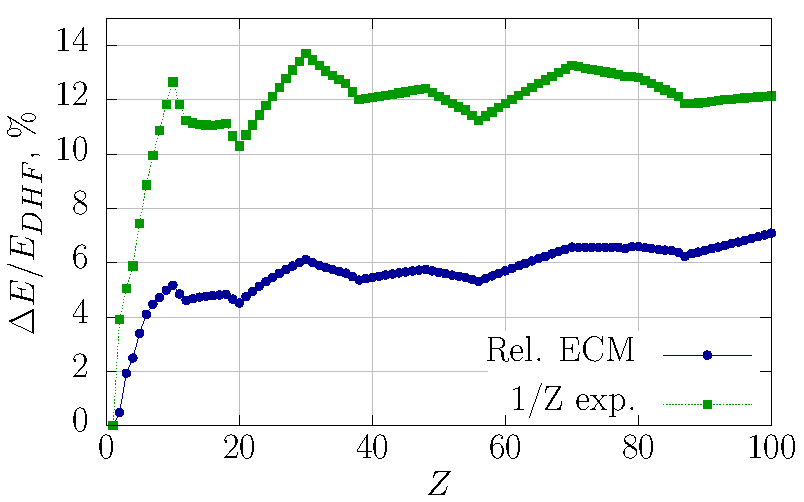
\includegraphics[width=69mm]{Graphs/Error_comparison.pdf}}
 \caption{Relative errors of the total binding energies calculated with the ECM as compared to the HF and DHF results~\eqref{Errorformula}. Left figure compares leading-order (blue) and single-electron second-order (green) ECM with the results of HF calculations~\cite{Saito2009836}. Right figure compares the leading-order D-ECM (blue) and first-order 1/Z expansion (green) to the results of DHF calculations~\cite{DESCLAUX1973311}. The corresponding numerical values of both non-relativistic and relativistic total binding energies are given in the Appendix~\ref{app:GroundStates}. This figure has been published as figure 1 in~\cite{Dzikowski_2021}.} \label{ErrorComparisonFigure}
\label{fig:my_label}
  \end{figure}

\begin{table}[b]%check values and add more digits to show differences
    \centering
    \begin{tabular}{cc|cccccc}
         Z &~$\rm{Element}$ &~$E^{(2)}_{\rm{single}}$ &~$E^{(2)}$ &~$\Delta E_{corr}$ &~$\rm{HF}$ &~$\rm{MCHF}$ & \rm{SDTQ}\\
         \hline
        \hline
         2 & He & -2.861 & -2.907 & 0.046 & -2.862 & -2.903 & 0.041 \\
         3 &Li & -7.411 & -7.462 & 0.051 & -7.433 & -7.477 & 0.044\\
         4 & Be & -14.52 & -14.69 & 0.165 & -14.57 & -14.67 & 0.093\\
         5 & B & -24.41 & -24.57 & 0.159 & -24.53 & -24.65 & 0.121\\
         6 & C & -37.49 & -37.64 & 0.148 & -37.69 & -37.84 & 0.150\\
         7 & N & -54.11 & -54.31 & 0.195 &-54.40 & -54.58 & 0.180\\
         8 & O & -74.38 & -74.65 & 0.268 & -74.81 & -75.05 & 0.245\\
         9 & F & -98.82 & -99.16 & 0.343 & -99.41 & -99.72 & 0.308\\
         \hline
    \end{tabular}
    \caption{Comparison of the second order single electron and double electron ground state energies with the single-configuration and multi-configuration numerical Hartree-Fock results.~$\Delta E_{corr}$ represent the electron-electron correlation energy calculated as the difference between the~$E^{(2)}_{\rm{single}}$ and~$E^{(2)}$, while SDTQ lists the corresponding Hartree-Fock result.}
    \label{tab:correlations}
\end{table}

This shows that the leading-order ECM and D-ECM give a particularly useful initial approximation to the orbitals of multi-electron atoms, and can be used a starting point for high-precision calculations, including those based on the HF method.

Following the considerations of section~\ref{sec:Green}, we can include electron-electron correlations, that is the double-electron second-order correction to the ECM. The resulting values of binding energy are in some cases already more accurate than the ones coming from the HF method and so have to be compared to the much more sophisticated MCFH procedure. Results for the first 10 neutral atoms are presented in table~\ref{tab:correlations}. Nevertheless, despite the promising accuracy of the second-order ECM, the largest source of uncertainty remains the neglect of higher orders of perturbation.

	\begin{figure} 
		\centering
		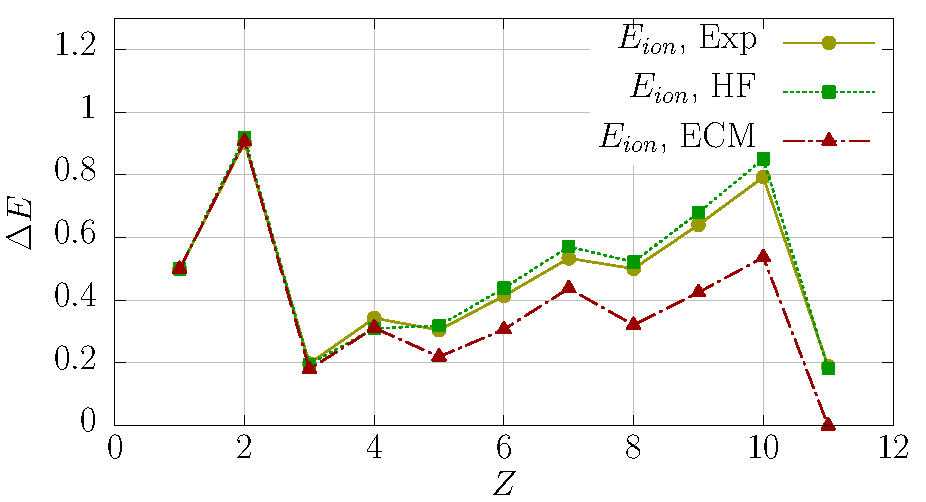
\includegraphics[width=120mm]{Graphs/Ionization.pdf} 
		\caption{Comparison of the first ionization energies of low-$Z$ neutral atoms, calculated with the full second-order ECM (red) with HF values~\cite{Saito2009836} (green) and experimental values from the NIST database~\cite{NIST} (yellow).} \label{Ionization}
		 		\end{figure}
	
	\begin{table}[b]%check values and add more digits to show differences
    \centering
    \begin{tabular}{cc|ccc}
         Z &~$\rm{Element}$ &~$\Delta E^{(2)}_{\rm{aff}}$ &~$\Delta E^{\rm{DFT}}_{\rm{aff}}$ &~$\Delta E^{\rm{exp}}_{\rm{aff}}$ \\
        \hline
        \hline
         1 & H & 0.87 & 0.84 & 0.75 \\
         2 & He & -1.27 & 0.03 & - \\
         3 & Li & 0.89 & 0.50 & 0.62 \\
         4 & Be & -4.23 & 0.03 & - \\
         5 & B & -4.30 & 0.43 & 0.28 \\
         6 & C & -2.81 & 1.39 & 1.26 \\
         7 & N & -6.64 & 0.23 & - \\
         8 & O & -6.19 & 1.83 & 1.46 \\
         9 & F & -5.3 & 3.74 & 3.40 \\
         \hline
    \end{tabular}
    \caption{Comparison of electron affinities of neutral atoms, between the full second-order ECM, DFT calculations~\cite{DFTaffinities}, and experimental measurements.} %[ref.].}
    \label{tab:Affinities}
\end{table}

\section{Ionization energies}

Since the number of electrons and the full nuclear charge~$Z$ are independent parameters in the ECM, it can also be used for the description of ions. By fixing~$Z$ and calculating the effective charge~$Z^*$ for electronic configurations with different numbers of electrons, we can describe positively-charged ions and find corresponding ionization energies. The first ionization energies for all atoms up to magnesium have been plotted in figure~\ref{Ionization}. The comparison to the HF calculation and experimental values shows that the relative error is larger than for energies themselves (as should be expected, since the errors have the same magnitude while values are much smaller), but the shape and general features of the ionization curve are well represented. This is not the case for other analytical approximations such as the TF model.

	Furthermore, by setting the full nuclear charge smaller than the number of electrons we can also investigate negative ions and their ionization energies, often referred to as electron affinities. This is a particularly interesting test of any computation scheme, as the extra electron of a negative ion is bound primarily by electron-electron correlation rather than the Coulomb force. Electron affinities of the first nine neutral atoms are presented in table~\ref{tab:Affinities}.
	
\begin{figure*}
  \centering  
  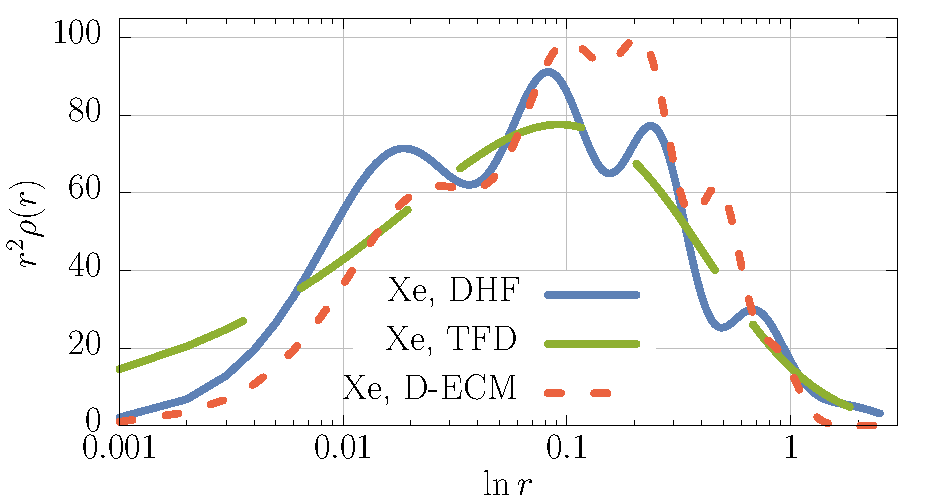
\includegraphics[height=37mm]{Graphs/xe_rel_rho.pdf}
 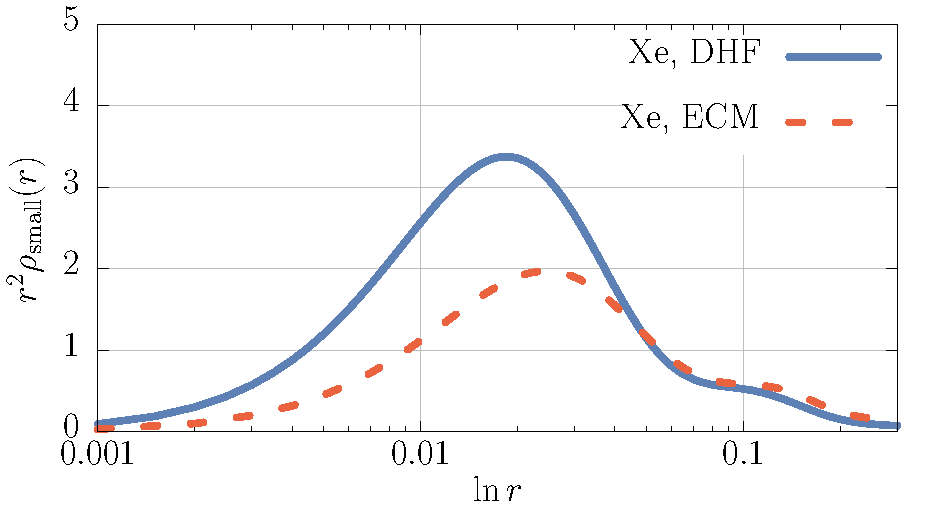
\includegraphics[height=37mm]{Graphs/xe_rel_rho_small.pdf}
  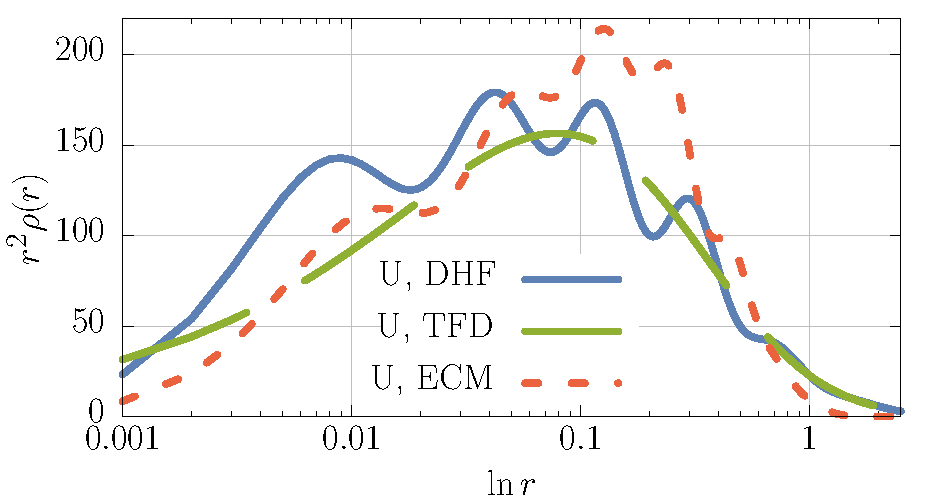
\includegraphics[height=37mm]{Graphs/u_rel_rho.pdf}
  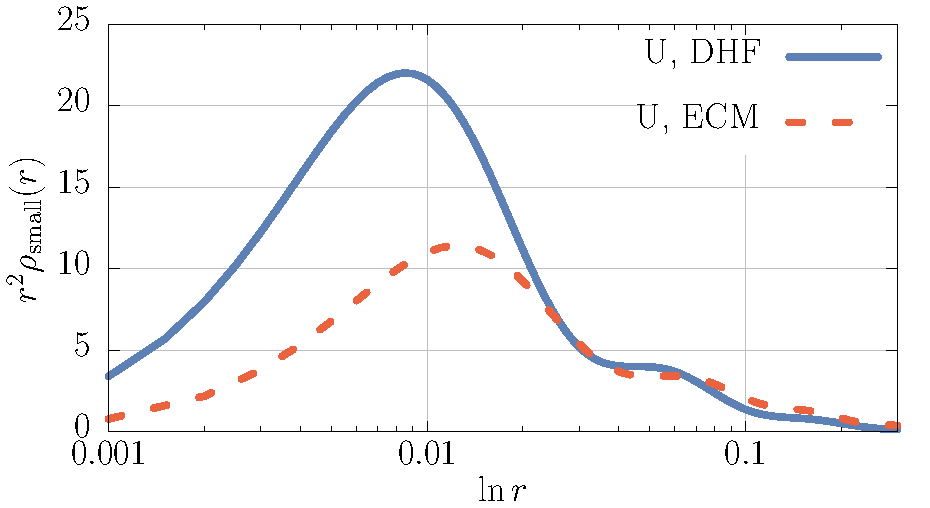
\includegraphics[height=37mm]{Graphs/u_rel_rho_small.pdf}
  \caption{Total radial electronic densities (left)
    and densities composed from the small components of the
    Dirac wave functions (right) of neutral
    xenon $_{54}$Xe (top) and neutral uranium
    $_{92}$U (bottom). Dashed, red line is the
    leading-order effective charge approximation, blue line
     represents the results of the numerical
    solution of DHF (obtained via GRASP2k~\cite{jonsson_new_2013,
      DYALL1989425}) and  green, long-dashed line stands for the TFD model. This figure has been published as figure 2 in~\cite{Dzikowski_2021}.}
  \label{Rel_rhoPlot}
\end{figure*}

\section{Electron densities}

In this section we demonstrate that the presented approach is suitable to provide useful approximations not only to the integral characteristics of the atom, but also to local ones, by investigating the ECM approximation to electron densities.

\subsection{Zeroth-order densities}

In the secondary-quantized representation, the density operator is given by
\begin{equation}
    \widehat{\rho}(r)=\sum_{\lambda,\lambda'}\psi_{\lambda}^\dag(r)\psi_{\lambda'}(r) \widehat{a}_{\lambda}^\dag \widehat{a}_{\lambda'}.
\end{equation}
Taking the expectation value of~$\widehat{\rho}$ with the leading-order wavefunctions of the ECM we get the leading order density
\begin{equation} \label{densityFormula}
    \langle\Psi^{(0)}|\widehat{\rho}(r)|\Psi^{(0)}\rangle = \sum_k \langle \lambda_k| \vec{r}\rangle \langle \vec{r}|\lambda_k \rangle,
\end{equation}
as a a sum of squares of hydrogen-like bound states. This means that the leading-order density is given by a simple combination of exponentials and polynomials,
allowing its use in numerical plasma~\cite{chung_flychk:_2005} or
description of ionization in particle-in-cell (PIC) computer codes
for laser-matter interactions~\cite{Arber_2015}. Furthermore, since the ECM, unlike the DHF and TF calculations, provides fully analytical expressions for electronic
densities and is therefore particularly useful for applications
requiring repeated calculations. Relatively simple expressions
resulting from our model can be incorporated into existing
software, used in the description of X-ray scattering on M\"{o}ssbauer
crystals~\cite{Sturhahn2000}. Explicit expressions are provided in Appendix~\ref{app:zeroDensities}.

In figure~\ref{Rel_rhoPlot} we plot the resulting
dependence of electronic densities on the radial coordinate~$r$ for
selected neutral atoms. Despite the fact that the effective charge
model underestimates the density for high~$r$, it agrees well with the
DHF result already in the leading-order
approximation. Contrary to the TFD model, it correctly
reproduces all of the qualitative features, including all density
oscillations and the overall asymptotic behavior. In addition, we
point out that the TFD model, unlike the
non-relativistic TF, does not have a
universal dependence on the charge of the nucleus~\cite{qua.560200311}. For this reason, in
order to obtain the electronic density, the TFD equation
needs to be repeatedly solved numerically, which is a nontrivial
procedure.

		\begin{figure} 
 			\centering
 			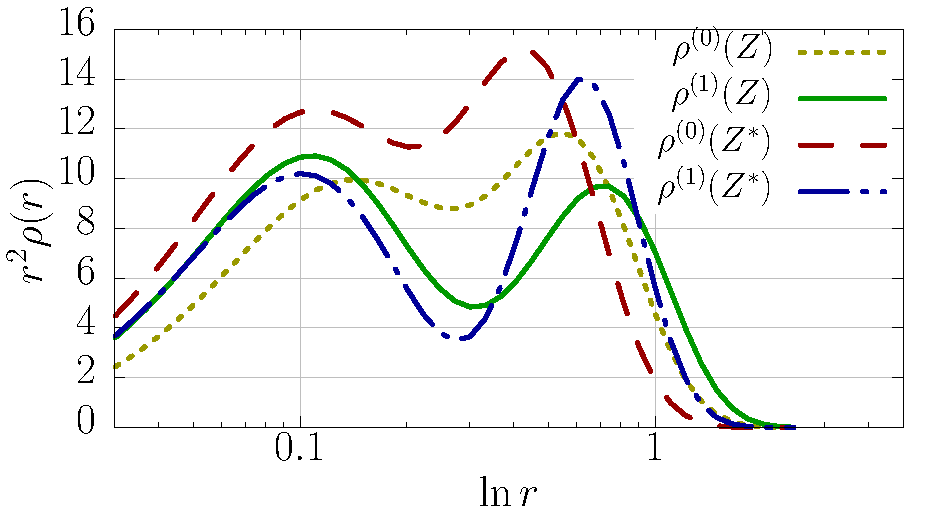
\includegraphics[width=69mm]{Graphs/Ne_rho.pdf} 
 			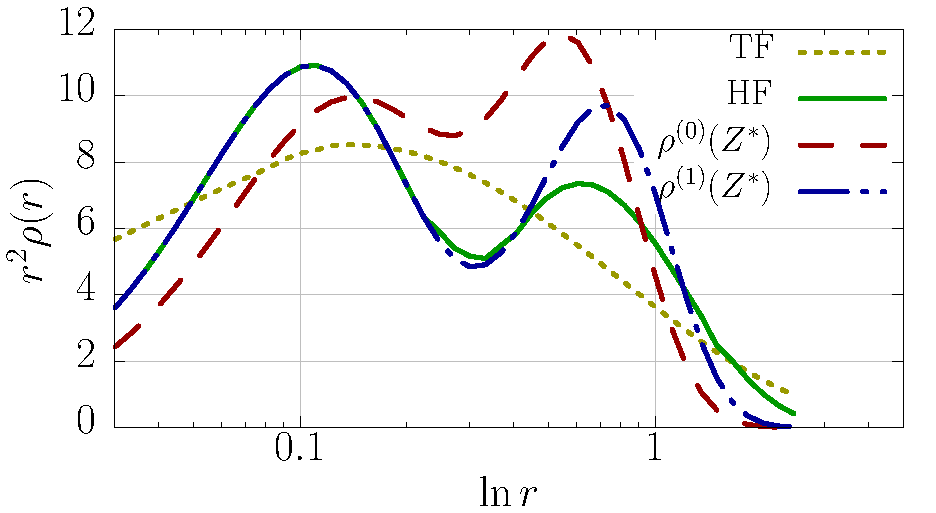
\includegraphics[width=69mm]{Graphs/Ne_rho2.pdf} 
 			\caption{Comparison of electron density of neutral neon using the zeroth-order and first-order ECM, with the zeroth-order and first order~$1/Z$ expansion (left), as well as with the HF results~\cite{jonsson_new_2013} and the TF model~\cite{LandauQM} (right). Red and blue are the zeroth- and first-order ECM calculations respectively. Yellow and green represent either the~$1/Z$ expansion (left) or the TF and HF results (right).} \label{NeonPlot}
 		\end{figure}

\subsection{First-order densities}

Using the the same approach as for energies, we can also easily derive analytical expressions for the first-order electron densities. Let's recall the perturbative expansion due to the operator~$W$ of our
multi-electron wave function
\begin{equation}
|\Psi \rangle = |\Psi^{(0)} \rangle + |\Psi^{(1)}\rangle +... = |\Psi^{(0)} \rangle + \sum_{\sigma} |\sigma\rangle \frac{\langle \sigma|\widehat{W}| \Psi^{(0)} \rangle}{E_0 - E_\sigma} +...~~,
\end{equation}
and split the intermediate states into single-electron and double-electron contributions just like in the calculation of energies
\begin{equation}
|\Psi \rangle = |\Psi^{(0)} \rangle + |\Psi^{(1)}_{\rm{single}}\rangle + |\Psi^{(1)}_{\rm{double}}\rangle...~~.
\end{equation}

Since~$\widehat{\rho}(r)$ it is a single-particle operator, only the single-electron part of~$\Psi^{(1)}$ will contribute to its expectation value, so that we have
\begin{align}\label{FirstDensityEq}
\widehat{\rho}(r)_{\Psi}^{(1)}&=\langle\Psi^{(0)}+\Psi^{(1)}_{\mathrm{single}}|\widehat{\rho}(r)|\Psi^{(0)}+\Psi^{(1)}_{\mathrm{single}}\rangle \nonumber
\\
&=\langle\Psi^{(0)}|\widehat{\rho}(r)|\Psi^{(0)}\rangle + 2\langle\Psi^{(0)}|\widehat{\rho}(r)|\Psi^{(1)}_{\mathrm{single}}\rangle + \langle\Psi^{(1)}_{\mathrm{single}}|\widehat{\rho}(r)|\Psi^{(1)}_{\mathrm{single}}\rangle \nonumber
\\
&= \sum_k \langle \lambda_k| \vec{r}\rangle \langle \vec{r}|\lambda_k \rangle + 2\sum_{l,k} \langle \lambda_k(r) | \Psi^{(1)}_{\mathrm{single},\lambda_l}(r) \rangle .
\end{align} 

Just as for energies, we can make use of the RCGF, to get the explicit expression for the first order wave function, as
\begin{equation} \label{1wave}
|\Psi^{(1)}_{\mathrm{single}}\rangle &= \sum_k |\Psi^{(1)}_{\mathrm{single},\lambda_k} \rangle = \sum_k \widetilde{G}_{\lambda_k} \widehat{W}^{(1)} |\lambda_k \rangle + \sum_{k,l \neq k} \widetilde{G}_{\lambda_k} \langle \lambda_l |\widehat{W}^{(2)}| \lambda_k \lambda_l \rangle,
\end{equation}
with implied exchange integrals.

\begin{figure*}
  \centering  
  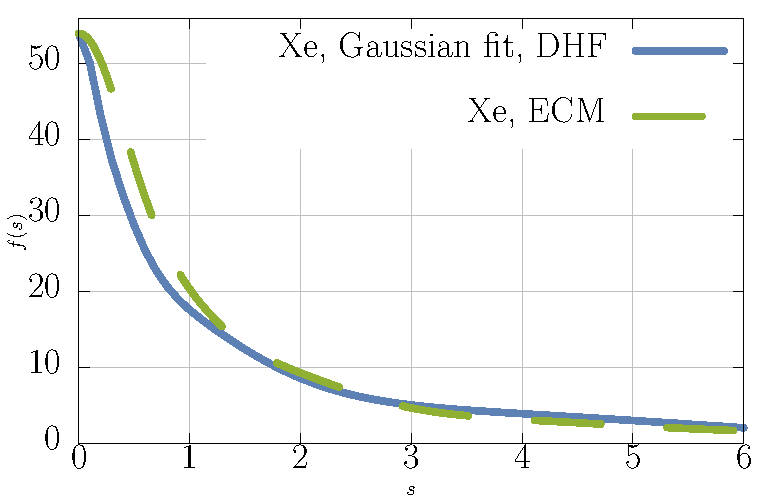
\includegraphics[width=69mm]{Graphs/asf_Xe.pdf}
  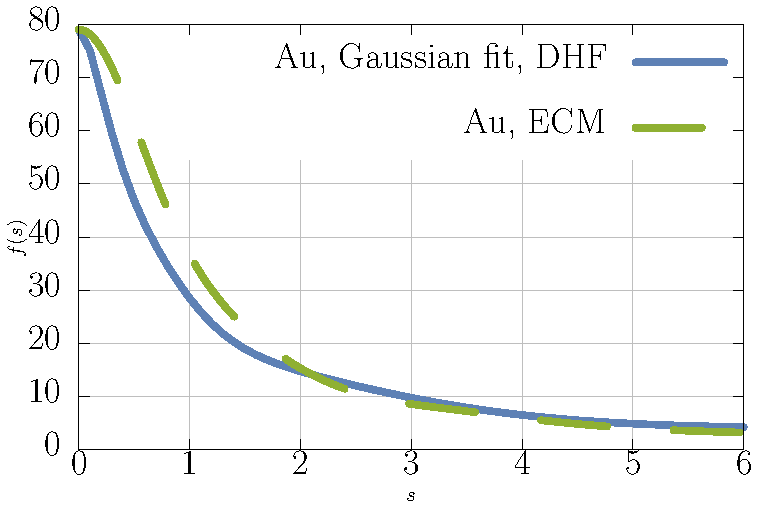
\includegraphics[width=69mm]{Graphs/asf_Au.pdf}
  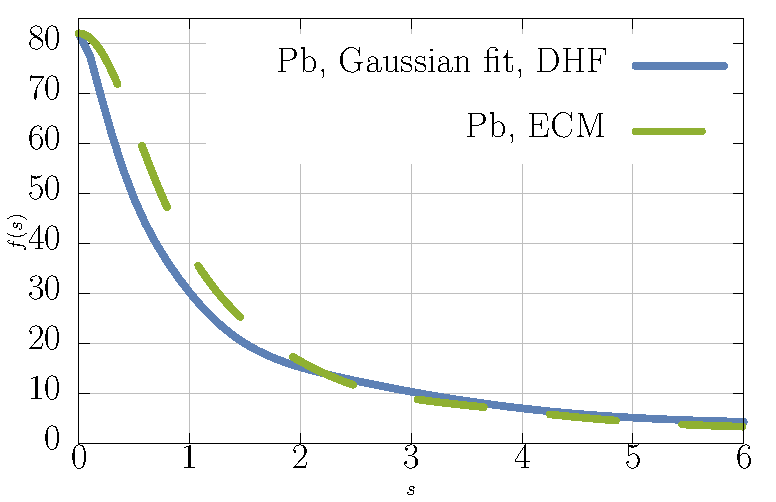
\includegraphics[width=69mm]{Graphs/asf_Pb.pdf}
  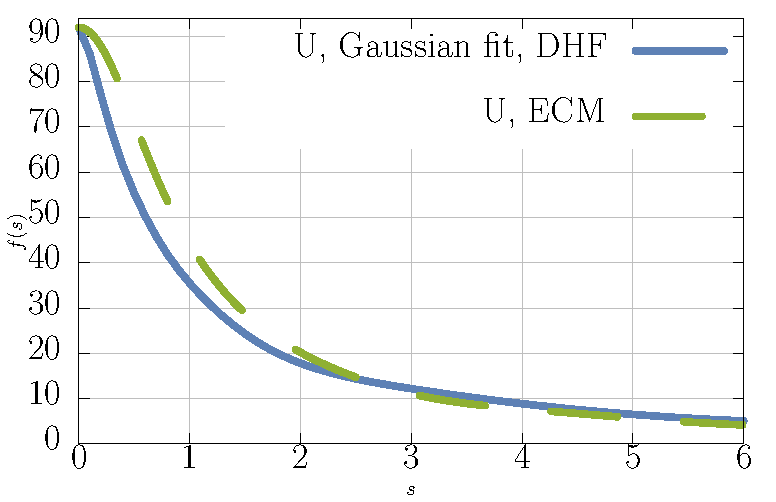
\includegraphics[width=69mm]{Graphs/asf_U.pdf}
  \caption{Atomic scattering factors of neutral xenon
   ~$_{54}$Xe, gold~$_{79}$Au, lead
   ~$_{82}$Pb and uranium~$_{92}$U atoms, as a
    function of the scattering parameter
   ~$s = \sin\theta / \lambda,\ [\textup{\AA}^{-1}]$, with~$\theta$
    being Bragg's angle. The quantity~$s$ is related to the absolute
    value of~$q$ from Eq.~(\ref{eq:15}) as
   ~$q = 4\pi s \cdot 0.529177$. Dashed, green line is the analytic
    result via Eq.~(\ref{eq:15}) of the ECM, while the solid
    blue curve is a Gaussian fit of DHF from
   ~\cite{DHFscatter}. This figure has been published as figure 4 in~\cite{Dzikowski_2021}.}
  \label{fig:ASF}
\end{figure*}

As an example, we have plotted the radial dependence of the electronic density of the neutral neon atom in figure~\ref{NeonPlot}. The left plot compares the ECM with the~$1/Z$ expansion (wchich corresponds to setting~$Z=Z^*$). We can see that the difference between them is significant and that the effective charge adjusts the width and height of the density plot. However, it also shows, that the relative height of subsequent density maxima can only be obtained with first order corrections. The right plot meanwhile compares the ECM to the results of HF and TF calculations. It is clear that unlike the TF model, the ECM reproduces the full shell structure with correct number of density maxima already in the zeroth-order. Furthermore, the first-order density aligns very well with the results of the HF calculation, except for large radial distances, where the ECM slightly underestimates the decay rate.

It is instructive to consider, how each of the terms in~\eqref{FirstDensityEq} scales with the effective nuclear charge, to see that subsequent terms do indeed get smaller rather quickly, ensuring fast convergence of the perturbation series. As explained in chapter~\ref{ch:ECM}, the charge/scale invariance of the Schr\"{o}dinger equation leads to simple scaling of wavefunctions and potentials:
\begin{align}
    \Psi_{\lambda}(r) \propto (Z^*)^\frac{3}{2},~~~~~~~~~~~~G(x,y) \propto Z^*,~~~~~~~~~~~~W_{k,\lambda,\lambda} \propto Z^*.
\end{align}
This in tern translates to scaling of density elements containing~$\widehat{W}^{(2)}$, as
\begin{equation}
\langle\Psi^{(0)}|\widehat{\rho}(r)|\Psi^{(0)}\rangle \propto (Z^*)^3 ,
\end{equation} 
\begin{equation}
\langle\Psi^{(0)}|\widehat{\rho}(r)|\Psi^{(1)}\rangle \propto (Z^*)^2 ,
\end{equation} 
\begin{equation}
 \langle\Psi^{(1)}|\widehat{\rho}(r)|\Psi^{(1)}\rangle \propto Z^* .
\end{equation} 
Elements containing~$\widehat{W}^{(1)}$ scale in the same way, with an extra factor of~$(Z-Z^*)$.

\section{Atomic scattering factors}
\label{sec:atom-scatt-fact}

Another example of a useful observable characteristic that can be easily approximated using the ECM, are the atomic scattering factors. They
are usually expressed~\cite{hau2012high} as the Fourier transforms of electronic density
\begin{align}
  f(\vec{q}) = \int \rho(\vec{r})e^{i \vec{q} \cdot \vec{r}}
  d\vec{r}, \label{eq:15}
\end{align}
which in the leading-order can be easily be calculated analytically (see
Appendix~\ref{app:scatter} for further details).

The atomic scattering factors are very important for crystallography
and X-ray physics, since the crystal polarizability~$\chi$ as the
function of X-ray frequency~$\omega_{\mathrm{r}}$, can be evaluated by
employing the following relation~\cite{ahmadi_feranchuk_2013}
\begin{align}
  \chi(\vec g, \omega_{\mathrm{r}}) = \frac{4 \pi S(\vec g)}{\Omega_{0}
  \omega_{\mathrm{r}}^{2}}
 f(\vec g), \label{eq:17}
\end{align}
where~$\Omega_0$ is the volume of a crystal cell,~$\vec g$ the
reciprocal lattice vector and~$S(\vec g)$ the structure factor of the
crystal.

In figure~\ref{fig:ASF} we present the results for neutral
xenon~$_{54}$Xe, gold~$_{79}$Au, lead~$_{82}$Pb and uranium~$_{92}$U
atoms. Our analytical expressions for atomic scattering factors are
comparable to the DHF calculation to within~$25\%$. At the same time, they are much more convenient to work with, being composed of finite sums of elementary functions rather than Gaussian fits to specific pre-calculated points.

\section{Highly charged ions}
\label{sec:highly-charged-ions}

In recent years there has been particular interest~\cite{IonsInterest} in the study both theoretical~\cite{IonsTheory} and experimental~\cite{IonsExperiment} of highly charged ions (HCI). Applications have been found in many different areas of modern physics, from optical clocks~\cite{IonsClocks} to fundamental physics~\cite{IOnsFundamental}. Since higher orders of the ECM are proportional to decreasing powers of~$Z$ and~$Z^*$, it naturally becomes more accurate in describing HCI, as compared to neutral atoms.

The results of the calculation of leading-order electronic densities of HCI are presented
in figure~\ref{fig:HCI}. The electronic densities calculated using the ECM, despite being
very simple analytical expressions,
coincide remarkably well with the ones obtained from numerical
solutions of the DHF equations.

\begin{figure*}
  \centering  
  \subfigure{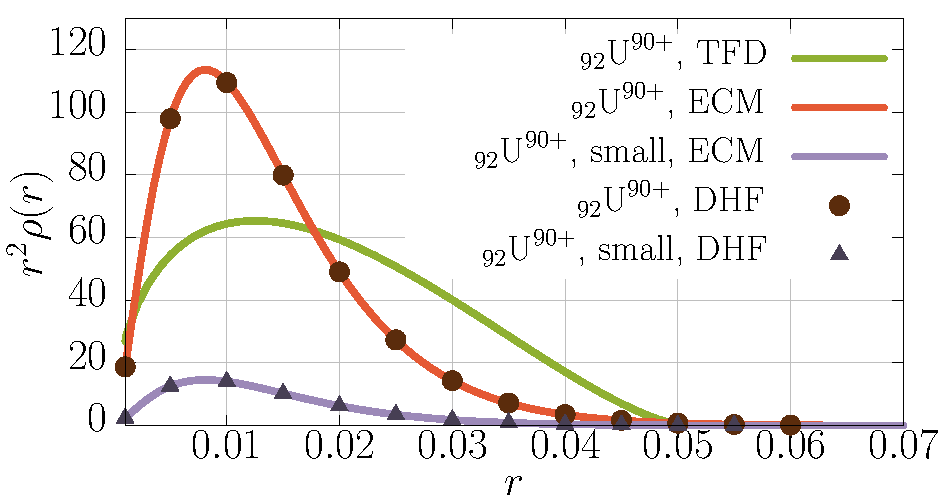
\includegraphics[width=69mm]{Graphs/helu_rel_rho.pdf}}
  \subfigure{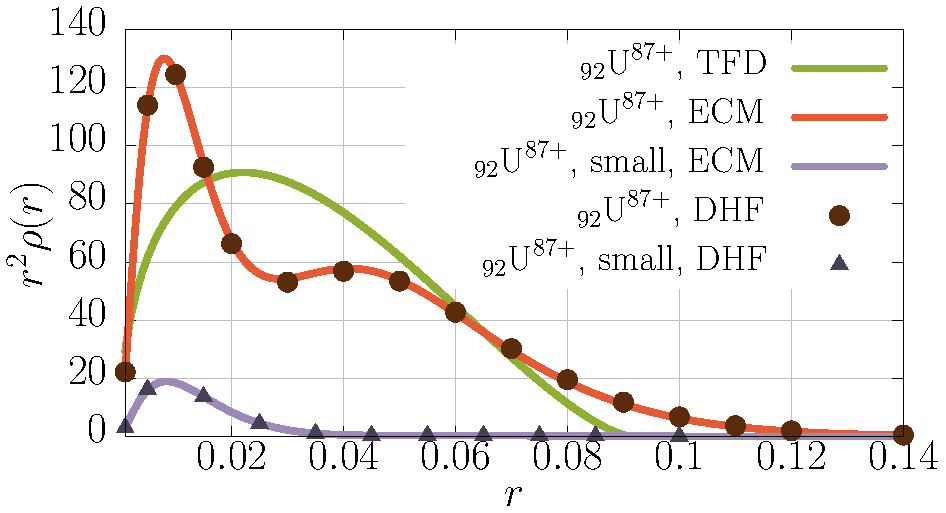
\includegraphics[width=69mm]{Graphs/blu_rel_rho.pdf}}
  \caption{Total and small component electronic
    densities of highly charged uranium \changeR{$_{92}$U$^{90+}$ and
     ~$_{92}$U$^{87+}$}. \changeR{Red (total) and purple (small)} lines are the \changeR{leading-order}
  ECM \changesR{densities},  \changeR{black circles (total) and black triangles (small) represent} results of the DHF \changeR{densities} (obtained via GRASP2k
   ~\cite{jonsson_new_2013, DYALL1989425}),  and the solid green stands for TFD model. This figure has been published as figure 3 in~\cite{Dzikowski_2021}.}
  \label{fig:HCI}
\end{figure*}

\section{Photoionization cross-section}
\label{sec:photo-ionis-cross}	

As one more practical application of the ECM, we
present the calculation of the total cross section for the
photoionization of a multi-electron atom. From first principles it can
be shown~\cite{PhysRev.134.A898}, that within the dipole approximation,
the differential cross-section for a photon with momentum~$k$ to
overcome an ionization energy~$E_0$ and produce an outgoing electron
with momentum~$p$ can be calculated according to
\cite{mikhailov1969relativistic}
\begin{equation}\label{PICformula}
  \frac{d \sigma}{d \Omega} = \frac{\alpha p (k+E_0)}{2 \pi k}
  \left|\int \psi^{\dagger}_f(\vec
    r)\vec{\alpha}\psi_i(\vec r) d\vec{r}\right|^2,
\end{equation}
where~$\psi_i$ is the initial bound-state wave function and the final
wave function can be described, as
\begin{equation}
  \psi_f(\vec r) = 4\pi \sum_{\kappa',m'}
  \xi_{\kappa',m'}\left(\frac{\vec{p}}{p}\right)e^{-i
    \delta_{\kappa'}}\psi_{\rm free}(\vec r),
\end{equation}
where~$\xi$ are normalized spinors~\cite{lifshitz1974relativistic},
describing the angular distribution and polarization of the outgoing
electrons, and~$\delta_{\kappa'}$ are phase shifts, ensuring outgoing
solutions.

Within the ECM,~$\psi_i$ and~$\psi_{\rm{free}}$ are
described by negative and positive-energy solutions to the Dirac
equation for hydrogen with relevant effective charge. Summing over all
electrons in a given atom or ion allows us then to analytically
calculate the total effective cross-section for the photoionization
process within the leading-order ECM (see Appendix~\ref{app:photo} for details).

In the presented calculation both initial and final wave functions have
been described using the same value of effective charge, so that they correspond to the same
effective potential. It is possible because the total cross-section
includes the summation over a full set of intermediate electron
excitations. The same approximation was employed in~\cite{YEH19851}.  On the other hand, the ionization
energies~$E_k$ are calculated separately for each electron, by finding
the "valence effective charge"~$Z^*_k$, defined by requiring the first
order correction to~$E_k$ to vanish. Hence it can be found by solving
\begin{equation}
  \Delta E^{(1)}_{\lambda_0}(Z^*_k)-\Delta E^{(1)}_{\lambda_k}(Z^*_k)=0,
\end{equation}
where~$\lambda_0$ is the ground state configuration and~$\lambda_k$
the final configuration, i.~e. without the ionised electron.
Figure~\ref{fig:PIC} presents the comparison of the results for two
example atoms with the analogous non-relativistic calculation, as well
as results of the Hartree-Fock-Slater (HFS) calculations~\cite{YEH19851}. It can be seen that shifting to a relativistic
description improves the accuracy of such calculation. The results
show that the ECM gives reasonable qualitative
description and can be used for approximating physical characteristics
dependent on transition matrix elements.

\begin{figure*}
	\centering  
	\subfigure{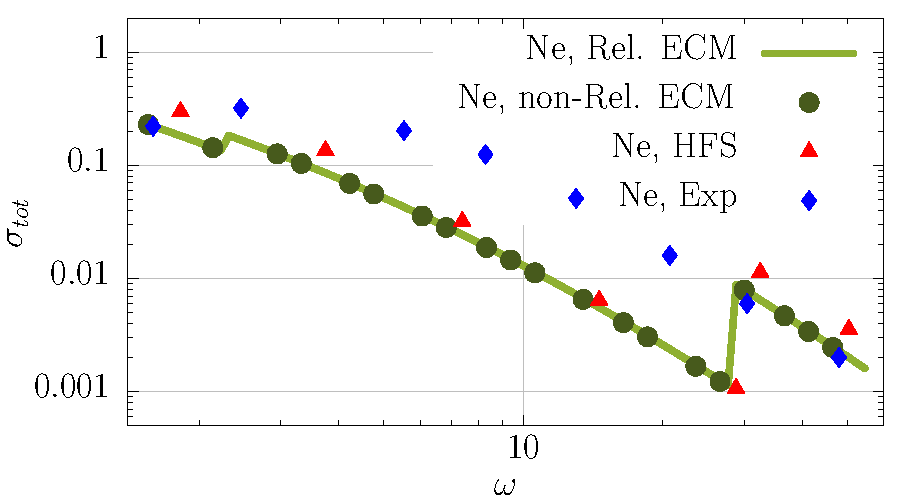
\includegraphics[width=69mm]{Graphs/photo_neon.pdf}}
	\subfigure{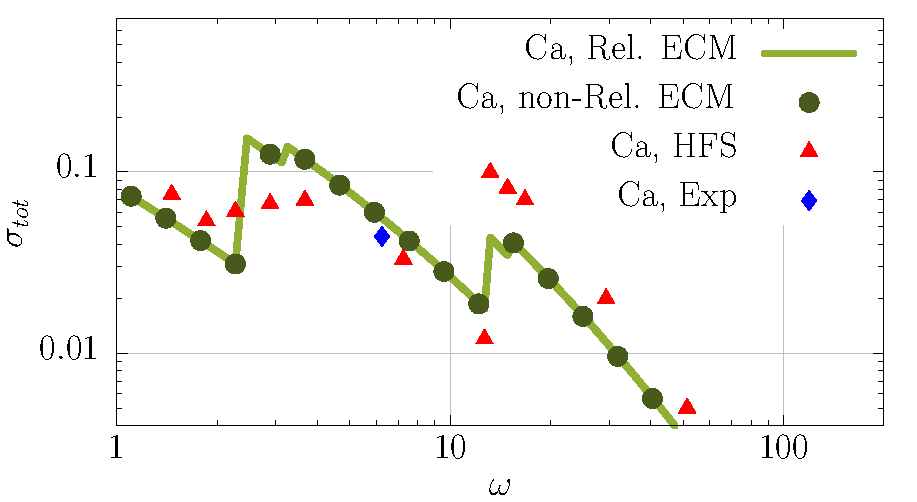
\includegraphics[width=69mm]{Graphs/photo_calcium.pdf}}
	\caption{Comparison of the ECM (circles)
		and D-ECM (solid) calculation of the total
		photoionization cross-section for neon~$_{10}$Ne (left)
			and calcium~$_{20}$Ca (right). Hartree-Fock-Slater calculation
		results are marked with red triangles and taken from~\cite{YEH19851}.Experimental data are taken
			from~\cite{MARR1976497} for neon and from~\cite{L_rch_1999} for calcium. This figure has been published as figure 5 in~\cite{Dzikowski_2021}.}
	\label{fig:PIC}
\end{figure*}

\section{Transition probabilities}
\label{sec:TP}

Transitions between electronic states are observed as emission lines in the spectrum of a given atom or molecule. The observed intensity is related to the probability of the transition, which is usually expressed per unit time ($\rm{sec}^{-1}$). For the purposes of theoretical analysis it is more convenient to analyse atomic transitions in terms of corresponding dimensionless quantities called oscillator strengths, which can be defined mathematically, as~\cite{OscillatorsDefinition}
\begin{equation}
    f = \frac{1}{8 \pi^2} g \lambda A^2,
\end{equation}
where~$g$ is the ratio of statistical weights of the involved atomic states,~$\lambda$ the corresponding wavelength and~$A$ the Einstein coefficient~\cite{EinsteinCoeff}.

The corresponding cross-section is then given by~\cite{EinsteinCoeff}
\begin{equation}
\sigma = \frac{\alpha \pi}{2} f \phi_{\omega},
\end{equation}
where~$\phi_{\omega}$ is the normalized angular frequency distribution \footnote{Even though oscillator strengths are defined so as to represent the normalized probability of transition, they can in some special cases be larger that unity~\cite{HENS2008391}.}.

\subsection{Non-relativistic calculation of transition probabilities}
	
	Using the Schr\"{o}dinger Hamiltonian, the oscillator strength of E1 transitions in the dipole representation between states described by the wavefunctions~$\psi_i$ and~$\psi_f$ can be calculated according to~\cite{demtroder2002laser}
\begin{equation}
    f = 2(E_f-E_i) \left|\langle \psi_i|\vec{r}|\psi_f \rangle \right|^2,
\end{equation}
where~$\vec{r}$ is a vector of all of the spatial coordinates involved (and so dimension~$3N$).

Within the leading-order ECM, we have:
\begin{align}
    &\Delta E (Z^*) \sim (Z^*)^2 \Delta E\\
    &\psi(r) \sim (Z^*)^{3/2}\psi(Z^* r),
\end{align}
which makes the leading order oscillator strengths independent of effective charge
\begin{equation}
    f^{(0)} \sim (Z^*)^0,
\end{equation}
and by extension independent of the total charge~$Z$. For these reason ECM can only be used to approximate oscillator strengths when higher orders are included. The first order correction to the wavefunctions is given by
\begin{equation}
    \psi^{(1)}(r) = \psi_0 W \widetilde{G}_{\psi_0},
\end{equation}
where the Greens function sums over all virtual states differing from~$\psi^{(0)}$ by at most two electrons. However since~$\vec{r}$ is a single-electron operator, only states that differ by one electron from either~$\psi_i$ or~$\psi_f$ will contribute in the first order. That is, for a transition
\begin{equation}
    |\lambda_1 ... \lambda_{n-1}, \lambda \rangle \rightarrow |\lambda_1 ... \lambda_n,\chi \rangle,
\end{equation}
the first order correction to~$\langle \psi_i^{(0)}|\vec{r}|\psi_f^{(0)} \rangle$ is given in its entirety by:
\begin{align}
   \Delta f^{(1)} =& \sum_i \langle \lambda \lambda_i|\widehat{W}|\lambda_i \rangle \widetilde{G}_{\lambda} \vec{r} | \chi \rangle +\langle \chi \lambda_i|\widehat{W}|\lambda_i \rangle \widetilde{G}_{\chi} \vec{r} | \lambda \rangle \nonumber
   \\
   &+ \sum_{i,j} \langle \lambda \lambda_i|\widehat{W}|\chi \rangle \widetilde{G}_{\lambda_i} \vec{r} | \lambda_j \rangle  + \langle \chi \lambda_i|\widehat{W}|\lambda \rangle \widetilde{G}_{\lambda_i} \vec{r} | \lambda_j \rangle 
\end{align}
with implied anti-symmetric exchange.

Corresponding results of the oscillator strengths for the two primary transitions in the low-$Z$ helium-like ions, namely~$1s^2 \rightarrow (1s2p)^1P_1$ and~$1s^2 \rightarrow (1s3p)^1P_1$ are presented in figure~\ref{OscillatorPlot}. We can see that the dependence on nuclear charge, absent from the zeroth-order result, is correctly reproduced in first order, with the accuracy improving with increasing charge.

\begin{figure}
    \centering
    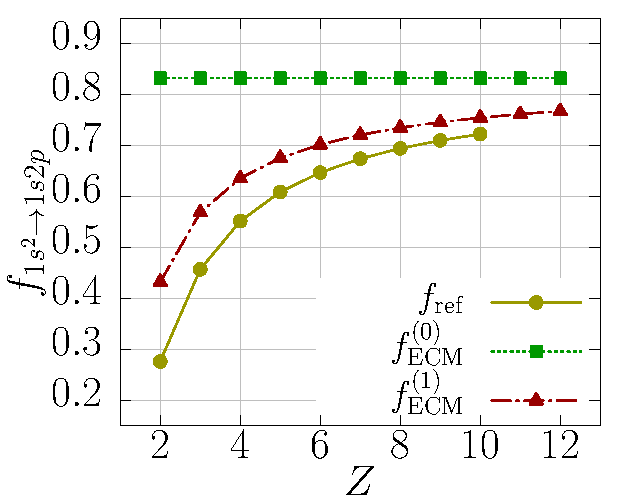
\includegraphics[width=69mm]{Graphs/OscillatorHe1s2p.pdf}
    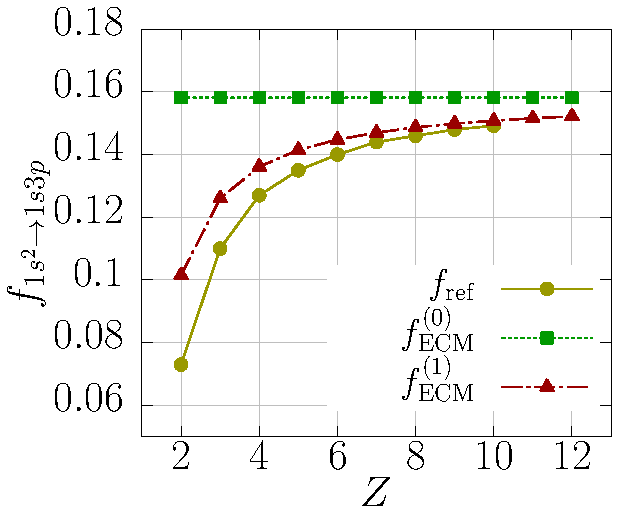
\includegraphics[width=69mm]{Graphs/OscillatorHe1s3p.pdf}
    \caption{Comparison of the zeroth-order (green) and first-order (red) oscillator strengths for the~$1s^2\rightarrow 1s2p$ (left) and~$1s^2\rightarrow 1s3p$ (right) transitions in helium-like ions with the corresponding reference values from the NIST database~\cite{NIST}.}
    \label{OscillatorPlot}
\end{figure}

\subsection{Gauge invariance of matrix elements}

Oscillator strengths can be expressed in terms of position matrix elements as~\cite{demtroder2002laser}
\begin{equation}
f_{i \rightarrow j} = \frac{2}{3} \frac{\Delta E_{ij}}{g_i} |\langle \psi_i|\vec{r}|\psi_j \rangle|^2 ,
\end{equation}
or in terms of momentum matrix elements as
\begin{equation}
f_{i \rightarrow j} = \frac{2}{3} \frac{1}{g_i \Delta E_{ij}} |\langle \psi_i|\vec{p}|\psi_j \rangle|^2 ,
\end{equation}
where~$\Delta E_{ij}$ is the energy difference between the two states between which the transition occurs, and~$g_i$ is the statistical weight of the state~$i$.

In principle, the two formulas above should be consistent (that is produce the same~$f$), however this is often not the case for many calculation schemes, because of incompatible numerical approximations. In fact, the equation obtained by equating the above two
\begin{equation} \label{consistency}
|\langle \psi_i|\vec{p}|\psi_j \rangle| = \Delta E_{i j} |\langle \psi_i|\vec{r}|\psi_j \rangle|,
\end{equation}
is sometimes used as an accuracy check of the approach used. In our case, it is trivially satisfied in the zeroth order, since by ground rules of quantum mechanics we always have
\begin{equation}
\widehat{p} = i [\widehat{H}_0,\widehat{r}] = i (\widehat{H}_0 \widehat{r} - \widehat{r} \widehat{H}_0),
\end{equation}
and if we multiply this relation by~$| \lambda \rangle$ states on both sides (which are exact eigenfunctions of~$\widehat{H}_0$), we immediately get (\ref{consistency}). The question of whether it is satisfied in the full second order energy calculation is less obvious, but can relatively easily be verified numerically.

\subsection{Relativistic calculation of transition probabilities}

For high-$Z$ atoms and ions the relativistic corrections to transition probabilities become important. An even more pronounced feature of the Dirac theory is that many of the non-relativistically forbidden transitions become possible. In particular, the so-called magnetic transitions, that is those where the multipole of the photon field causing the transition is not equal to the change in the angular momentum quantum number. The full relativistic calculation is somewhat more involved due to the non-diagonal interaction between electron spinors and the photon field. Nevertheless, using the Dirac Hamiltonian, the transition cross-section between the states described by~$\psi_i$ and~$\psi_f$ can be found according to~\cite{mikhailov1969relativistic}
\begin{equation}
   \frac{d\sigma}{d\Omega} = \frac{\alpha}{2\pi}\Delta E_{ij}|\langle\psi_i|\vec{\alpha} \cdot \vec{e}e^{i \vec{k} \cdot \vec{r}}|\psi_f\rangle|^2,
\end{equation}
where~$\vec{e}$ is the polarization vector of the photon field and the Dirac vector of matrices is given by~\cite{lifshitz1974relativistic}
\begin{equation}
    \vec{\alpha}=\left(\begin{matrix}0&\vec{\sigma}\\\vec{\sigma}&0\end{matrix}\right).
\end{equation}
The simplest way to evaluate the above equation in practice is by expanding the plane-wave photon field in Bessel functions~\cite{AS}
\begin{equation}
    e^{\ii \vec{k} \cdot \vec{r}} = 4\pi \sum_{m,l} i^l j_l \left(k r \right)Y^*_l^m\left(\frac{\vec{k}}{k}\right)Y_l^m\left(\frac{\vec{r}}{r}\right),
\end{equation}
and after averaging over polarizations, we eventually arrive at
\begin{equation}
    \frac{\alpha \Delta E_{ij}}{|\kappa|} \frac{(2J+1)(J+1)}{J} |\tau_J|^2,
\end{equation}
where for magnetic transitions we get
\begin{equation}
    \tau = i \frac{\kappa_i+\kappa_f}{\sqrt{J(J+1)}} C_J \int (\widetilde{G}_b(r)f_a(r)+f_b(r)\widetilde{G}_a(r))j_J(kr) r^2 dr,
\end{equation}
while for electric ones
\begin{align}
    \tau =i &\frac{\sqrt{J(J+1)}}{2J+1} C_J \nonumber
    \\
    \times& \int\Bigg(\left[1+\frac{\kappa_a-\kappa_b}{J+1}\right]\widetilde{G}_f f_i j_{J+1}(k r) - \left[1-\frac{\kappa_a-\kappa_b}{J+1}\right]\widetilde{G}_i f_f j_{J+1}(k r) \nonumber
    \\
    &-\left[1+\frac{\kappa_a-\kappa_b}{J}\right]\widetilde{G}_f f_i j_{J-1}(k r)+\left[1-\frac{\kappa_a-\kappa_b}{J}\right]\widetilde{G}_i f_f j_{J-1}(k r)\Bigg)r^2 dr,
\end{align}
 where the matrix elements of the total angular momentum operator are given by
\begin{equation}
    C_J 
    %= \langle \psi_i|S_J|\psi_f \rangle = Natalia doesn't approve
    (-1)^{j_i-J-1/2}\sqrt{(2j_i+1)(2j_f+1)}\left(\begin{matrix}j_i&j_f&J\\\-1/2&1/2&0
    \end{matrix}\right)
\end{equation}

\begin{figure}
    \centering
    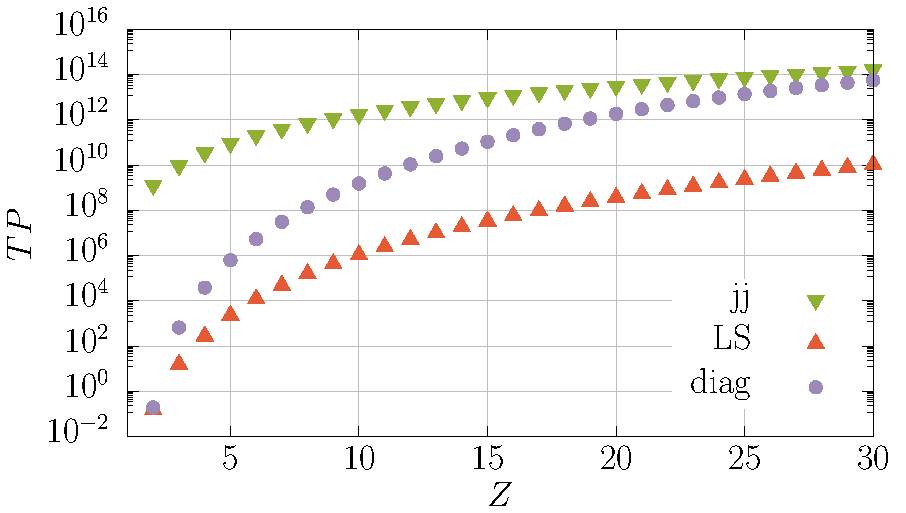
\includegraphics[width=130mm]{Graphs/LSvsjj.pdf}
    \caption{The probabilities of the~$1s^2 \rightarrow (1s 2p) {}^3P_1$ and~$1s^2 \rightarrow (1s_{1/2} 2p_{3/2})_1$ transitions are compared to the corresponding transition with exact coupling. It can be readily seen that~$LS$-coupling is accurate for small~$Z$, while~$jj$-coupling becomes more accurate as the nuclear charge increases. All data calculated with leading-order D-ECM.}
    \label{LSjjPlot}
\end{figure}

\section{Energies of excited states}
\label{sec:Coupling}

There remains one more question to be discussed - how to efficiently calculate excited energies. Excited states of atoms and ions tend to have much more degeneracy than the ground state and so one needs to be particularly careful about the definition of the specific zeroth-order electronic configurations. As mentioned in chapter~\ref{ch:secondECM}, in the case of multiple degenerate configurations, the multi-electron wavefunction can be obtained by diagonalizing the total Hamiltonian in the finite subspace spanned by the degenerate states. However since the number of possible configurations generally grows exponentially with the number of electrons, for the purpose of easy identification of states, approximate coupling schemes are often employed. In practice this means finding linear combinations of single-electron orbitals that result in definite values of the total quantum numbers of the multi-electron wavefunction.

\subsection{$LS$- vs.~$jj$-coupling}

The two simplest and most commonly used angular momentum coupling schemes are called~$LS$-coupling and~$jj$-coupling, referring to the specific quantum numbers that are fixed in the resulting configuration\footnote{By convention, small letters refer to quantum numbers of single-electron orbitals, while capital letters describe the total multi-electron wavefunction.}.

In the case of~$LS$-coupling the~$l$ and~$s$ quantum numbers of individual electrons add up to the total $L$ and $S$ of the multi-electron configuration respectively. For the purpose of evaluating relativistic corrections those can be further coupled to the total $J$ quantum number. For example, in the case of two-electron ions with one electron in the~$1s$ subshell and another in~$2p$, the possible~$LS-$coupled states are:
\begin{equation}
   (1s 2p) {}^1P_1,~~~~~~(1s 2p) {}^3P_1,~~~~~~(1s 2p) {}^3P_2.
\end{equation}

On the other hand, in the~$jj$-coupling scheme, the~$j$ quantum numbers of individual electrons add up to the total~$J$ quantum number of the multi-electron configuration. In the same example as above the three possible~$jj$-coupled states are:
\begin{equation}
   (1s_{1/2} 2p_{1/2})_1,~~~~~~(1s_{1/2} 2p_{3/2})_1,~~~~~~(1s_{1/2} 2p_{3/2})_2.
\end{equation}

\begin{figure}
    \centering
    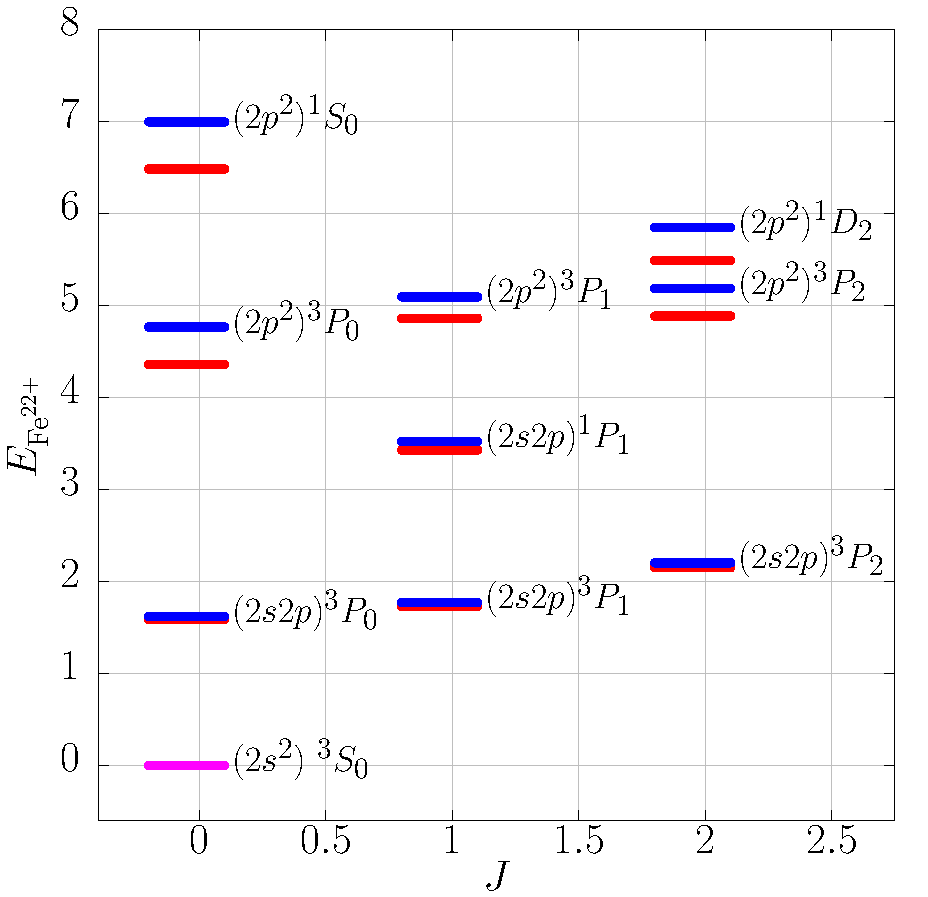
\includegraphics[width=69mm]{Graphs/ExcitedBerylium.pdf}
    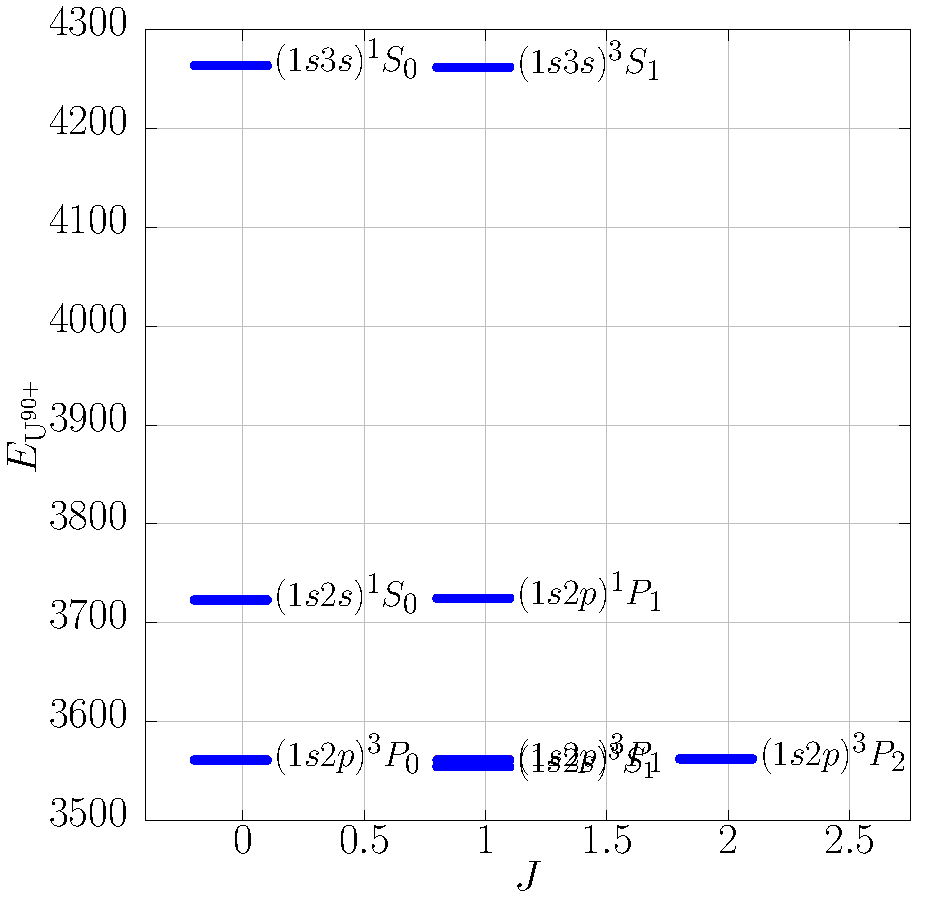
\includegraphics[width=69mm]{Graphs/ExcitedUlikeHe.pdf}
    \caption{Comparison of excited energies of~$_{26}$Fe${}^{22+}$ (left) and~${}_{92}$U${}^{90+}$ (right), calculated by diagonalizing a finite matrix in the leading-order ECM (blue) with references values (red). The reference values for~$_{26}$Fe${}^{22+}$ are taken from the NIST database~\cite{NIST} and for~${}_{92}$U${}^{90+}$ calculated with the  CI-DFS method~\cite{Tup2003OS}. The scale is fixed so that the energy of the ground state (pink) is equal to zero. Horizontal axis corresponds to total angular momentum quantum number of the multi-electron wavefunction. Numerical values given in Appendix~\ref{app:HCI}.}
    \label{ExcitedPlot}
\end{figure}


It is not always readily seen whether the~$LS$- and~$jj$-coupling scheme describe the same configurations. In this specific example only the third state is the same. The other two are related by the so-called~$LS$-$jj$ recoupling, which in this example happens to be
\begin{equation}
    \left(\begin{matrix}
    (1s 2p) {}^1P_1 \\
    (1s 2p) {}^3P_1
    \end{matrix}\right)
    =
    \frac{1}{\sqrt{3}}
    \left(\begin{matrix}
    \sqrt{2} & 1 \\
    1 & -\sqrt{2}
    \end{matrix}\right)
   \left(\begin{matrix}
    (1s_{1/2} 2p_{1/2})_1 \\
    (1s_{1/2} 2p_{3/2})_1
    \end{matrix}\right).
\end{equation}
In general, the $LS$-$jj$ recoupling is given by
\begin{equation}
    R_{LS \rightarrow jj} = \sqrt{(2L+1)(2S+1)(2j_1+1)(2j_2+1)}\left\{\begin{matrix}l_1&l_2&L\\s_1&s_2&S\\j_1&j_2&J\end{matrix}\right\},
\end{equation}
with the~$9j-$symbol defined in~\cite{9j}.

\subsection{State mixing}

It is important to emphasize that both of the above coupling schemes are approximations and the exact coupling can always be obtained by diagonalizing the Hamiltonian in the corresponding subspace. However, the resulting coefficients of the linear combination of single-electron orbitals, the so-called state mixing, depends on the nuclear charge~$Z$ and in the case of the ECM also influences the effective charge~$Z^*$. In practice, the~$LS$-coupling gives accurate predictions for low-$Z$ ions, while the~$jj$-coupling becomes more accurate as the nuclear charge increases. The transition cross-section calculation can be an interesting way of demonstrating that. As an example, in figure~\ref{LSjjPlot} the probabilities of the~$1s^2 \rightarrow (1s 2p) {}^3P_1$ and~$1s^2 \rightarrow (1s_{1/2} 2p_{3/2})_1$ transitions are compared to the corresponding transition with exact coupling for different values of~$Z$. It can be seen that the correct physical state, obtained from subspace diagonalization, corresponds to the~$LS$-coupled state only for~$Z \sim 2$, and then gradually gets closer to the~$jj$-coupled state as~$Z$ increases.

Despite the fact that the subspace diagonalization procedure is only necessary for degenerate states, it can also be useful in accounting for the mixing between states with small energy separation, that are nevertheless not strictly degenerate. This is because the perturbative corrections that these states contribute to each others values of energy are correspondingly larger. Since the subspace diagonalization procedure effectively accounts for all orders of perturbation coming from these states, it can describe low laying excited states of multi-electron atoms with good accuracy already in the leading-order. In figure~\ref{ExcitedPlot} we show the result of diagonalizing the~$1s^2 \{2s,2p,3s,3p\}^2$ subspace for be-like iron and the~$1s\{2s,2p,3s\}$ subspace for he-like uranium. Despite using  very small subspaces, both examples result in correct ordering of excited states already in the leading order, including all fine-structure states. 




\chapter{QED and nuclear corrections}
\addtocontents{toc}{\contentsline{chapter}{QED and nuclear corrections}{\protect\pageref{annotation}}}
\label{ch:Improvements}

This chapter presents the calculation of the leading-order contributions of the most important effects previously neglected in our formulation of the ECM. Specifically, the corrections to bound state energies coming from the Breit interaction, finite-nuclear-size effect and vacuum polarization. The results show good agreement with reference values already in the leading order.  

\section{Relativistic potentials}

The potentials used in our derivation of the ECM and D-ECM were all non-relativistic, that is, of the form~$\frac{1}{r}$. This makes them instantaneous and so a good description only of the interaction with the nucleus (since it is assumed stationary), %(what about magnetic interaction?!)
 but not of the interaction between electrons, when they are moving with relativistic velocities. A more accurate, fully relativistic form of the interaction between two charged particles can be derived using the theory of quantum electrodynamics (QED). The equations describing QED however, cannot be solved exactly, so in practice the resulting corrections have to be treated perturbatively. 
 
 In order to improve the form of the potential, one needs to understand which corrections are most relevant. For this reason let us first examine the scaling of different interactions and their respective corrections. In Schr\"odinger theory the interaction between the electrons and nucleus is proportional to the nuclear charge squared $Z^2$ (see~\eqref{SchrA}), while the first-order interaction between pairs of electrons (see~\eqref{SchrB}) is proportional to $Z$ (in the case of $Z^*=Z$)\footnote{It is conventional to factor out the powers of $Z$ and refer to the relative scaling of the electron-electron interaction to the electron nuclear interaction, as $1/Z$}. The difference between the Schr\"odinger and Dirac descriptions scales to leading order as $(\alpha Z)^2$ (see~\eqref{DiracA}), so we can say that the relativistic corrections are of the order $Z(\alpha Z)^2$. Notice however that, by using the fully relativistic D-ECM wavefunctions we have accounted for the electron-nucleus interactions to all orders in $(\alpha Z)$. 
 
 Interactions in QED are conveniently represented using Feynmann diagrams~\cite{FD}, where the leading-order interactions correspond to the exchange of a single virtual photon. In the case of two electrons, such interaction is described (in the limit of low frequency) by a potential of the form:
 \begin{equation}
     V(r) = \frac{1}{r_{ij}} + B_{ij},
 \end{equation}
 where $B_{ij}$ is an off-diagonal operator of the order $Z(\alpha Z)^2$, called the Breit operator~\cite{bethe2014quantum}. It contains magnetic interaction coming from electron's spin, as well as leading-order retardation effects (both electric and magnetic). A similar correction term can be written for the electron-nucleus interaction, but since we assume the nucleus to be stationary, the is no retardation and only the magnetic effect remains. Both of these are presented in figure~\ref{BreitFig}.

\section{Breit interaction}

Using the Dirac matrices, defined by~\eqref{DiracAlpha}, we can write the Breit operator as~\cite{bethe2014quantum}\footnote{This is the low frequency limit of the Breit operator. The full frequency dependent version - as implemented for example in the GRASP2k package - can be found in~\cite{Si2019CriticalEO}.}
\begin{equation}
B_{ij} = \frac{1}{2}\left(\frac{\vec{\alpha}_i \cdot \vec{\alpha}_j}{|\vec{r}_{ij}|}+\frac{(\vec{\alpha}_i \cdot r_{ij}) (\vec{\alpha}_j \cdot \vec{r}_{ij})}{|\vec{r}_{ij}|^3}\right),
\end{equation}
where the indices~$i,j$ label a pair of electrons, and the inner product runs through the three Dirac matrices~$\vec{\alpha} = (\alpha_1, \alpha_2, \alpha_3)$.

\begin{figure*}
  \centering  
\subfigure{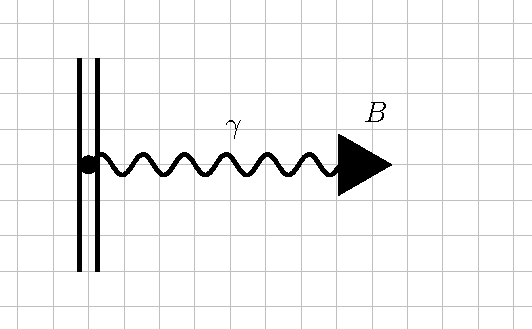
\includegraphics[width=69mm]{Graphs/NucleusBreitMagnetic.pdf}}
 % \hspace{10mm}
    \subfigure{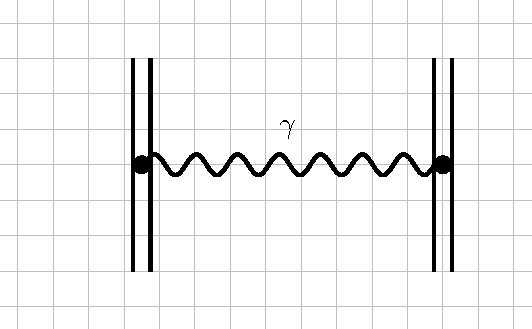
\includegraphics[width=69mm]{Graphs/BreitFeynmanLabeled.pdf}}
  \caption{Feynman diagrams of the leading-order magnetic interaction between an electron and the nucleus (left) and of the Breit interaction between two electrons (right). The double lines represent bound states of electrons in the field of the nucleus. The wiggly line is the photon propagator and triangle represents the interaction with the magnetic field of the nucleus.}
  \label{BreitFig}
\end{figure*}

The operator~$B_{ij}$ contains the $\frac{1}{r_{ij}}$ potential, as well as leading-order retardation effects and the magnetic interaction coming from electron's spin (notice that it involves off-diagonal elements in the standard representation). Similarly there is a magnetic interaction between the spin of the nucleus and that of the electrons, which in the leading order is described by an exchange of a single virtual photon. Both of these presented in figure~\ref{BreitFig}.

Since the two terms in the Breit operator are similar in magnitude~\cite{00018737000101191}, for our purposes we approximate the Breit operator as
\begin{equation}
B_{ij} \approx \frac{\vec{\alpha}_i \cdot \vec{\alpha}_j}{|\vec{r}_{ij}|}.
\end{equation}

We can then apply the Wigner-Eckhart theorem~\cite{sakurai2020modern} to the general case to get
\begin{align}
\langle \lambda_1 \lambda_2 | \frac{\vec{\alpha}_i \cdot \vec{\alpha}_j}{|r_i-r_j|} | \lambda_3 \lambda_4 \rangle &= \sum_i\frac{\langle \lambda_1 | \alpha^i | \lambda_3 \rangle \langle \lambda_2 | \alpha^i | \lambda_4 \rangle}{|r_1-r_2|} \nonumber
\\
&= 2\sum_{p,J} M_{pJ}(\overline{\lambda_3},\lambda_1)M_{pJ}(\lambda_2,\overline{\lambda_4})R_P(g_1 g_2 f_3 f_4) \nonumber
\\
&+2\sum_{p,J} M_{pJ}(\overline{\lambda_3},\lambda_1)M_{pJ}(\overline{\lambda_2},\lambda_4)R_P(g_1 f_2 f_3 g_4) \nonumber
\\
&+2\sum_{p,J} M_{pJ}(\lambda_3,\overline{\lambda_1})M_{pJ}(\lambda_2,\overline{\lambda_4})R_P(f_1 g_2 g_3 f_4) \nonumber
\\
&+2\sum_{p,J} M_{V}(\lambda_3,\overline{\lambda_1})M_{pJ}(\overline{\lambda_2},\lambda_4)R_P(f_1 f_2 g_3 g_4), \label{BreitFull}
\end{align}
with the angular part given by~\cite{PhysRev.154.17}
\begin{align}
M_{Jp}(\lambda_1,\lambda_2) = &\sqrt{3(2l_1+1)(2l_2+1)(2J+1)(2j_1+1)(2j_2+1)} \\
&\times\begin{pmatrix}
j_1 & j_2 & J
\\
-m_1 & m_2 & m_1-m_2
\end{pmatrix}\begin{pmatrix}
l_1 & l_2 & p
\\
0 & 0 & 0
\end{pmatrix}
\left\{\begin{matrix}
l_1 & 1/2 & j_1
\\
l_1 & 1/2 & j_1
\\
k & 1 & k
\end{matrix}\right\},
\end{align}
and the radial by
\begin{equation}
R_p(\psi_1 \psi_2 \psi_3 \psi_4) = \int \psi_1 (r_1) \psi_2 (r_2) \psi_3 (r_1) \psi_4 (r_2) \frac{r_<^p}{r_>^{p+1}}r_1^2r_2^2dr_1 dr_2,
\end{equation}
where the overline indicates a flip of the sign of the relativistic quantum number~$\kappa$.

Like in the Coulomb case, for a two-electron Slater determinant, we get a difference between direct and exchange terms
\begin{equation}
\langle \lambda_1 \lambda_2 | \frac{\vec{\alpha}_i \cdot \vec{\alpha}_j}{|r_i-r_j|} | \lambda_1 \lambda_2 \rangle = \langle \lambda_1 | \langle \lambda_2 | \frac{\vec{\alpha}_i \cdot \vec{\alpha}_j}{|r_i-r_j|} | \lambda_1 \rangle | \lambda_2 \rangle - \langle \lambda_1 | \langle \lambda_2 | \frac{\vec{\alpha}_i \cdot \vec{\alpha}_j}{|r_i-r_j|} | \lambda_2 \rangle | \lambda_1 \rangle,
\end{equation}
while the total contribution to the energy of a multi-electron atom can be written as
\begin{align}
    \langle \lambda_1 ... \lambda_n | \frac{\alpha_1 \cdot \alpha_2}{r_{12}} |\lambda_1 ... \lambda_n \rangle &= \sum_{i < j}^n \langle \lambda_i \lambda_j | \frac{\alpha_1 \cdot \alpha_2}{|r_1-r_2|} |\lambda_i \lambda_j \rangle \nonumber
    \\
    &= \frac{1}{2}\sum_{i,j}^n \langle \lambda_i \lambda_j | \frac{\alpha_1 \cdot \alpha_2}{|r_1-r_2|} |\lambda_i \lambda_j \rangle,
\end{align}
where the final form on the right hand side is most useful for deriving formulas for closed shells. 

Plugging in~\eqref{BreitFull}, we get the direct term as
\begin{equation}
\langle \lambda_1 | \langle \lambda_2 | \frac{\alpha_i \cdot \alpha_j}{|r_i-r_j|} | \lambda_1 \rangle | \lambda_2 \rangle = 8 \sum_p M_{pp}(\lambda_1,\lambda_1)M_{pp}(\lambda_2,\lambda_2)R_p(g_1 g_2 f_1 f_2).
\end{equation}
However since
\begin{equation}
\sum_m \begin{pmatrix} j & j & J\\-m & m & 0 \end{pmatrix} = 0,
\end{equation}
the sum over projections vanishes in this case for any value of~$p$
\begin{equation}
\sum_{m}M_{pp}(\lambda,\lambda)=0,
\end{equation}
so the direct term is zero for a closed shell.
The exchange term on the other hand becomes
\begin{align}
M_{\lambda_1 \lambda_2} = & \langle \lambda_1 | \langle \lambda_2 | \frac{\alpha_i \cdot \alpha_j}{|r_i - r_j|} | \lambda_2 \rangle |\lambda_1 \rangle \nonumber
\\
 = & 2\sum_{p} \big[\epsilon_{p }(\ovjrline{\lambda_1},\lambda_2)R_p(g_1 g_1 f_2 f_2) +\epsilon_{p }(\lambda_1,\overline{\lambda_2})R_p(f_1 f_1 g_2 g_2)2 \nonumber
 \\
 &+ f_{p}(\lambda_1,\lambda_2)R_p(g_1 g_2 f_1 f_2)\big].
\end{align}

\begin{table}[t]
\centering
\begin{tabular}{cc|lllr}
	Element & Z &~$E^{\rm{Br}}_{\rm{D-ECM}}(Z)$ &~$E^{\rm{Br}}_{\rm{D-ECM}}(Z^*)$ & $E^{\rm{Br}}_{\rm{DHF}}$ & $ \Delta E^{\rm{Br}}$\\
	\hline
	\hline 
	He & 2 & 0.00005 & 0.00003 & 0.00006 & 50\% \\
	Be & 4 & 0.00056 & 0.00034 & 0.00071 & 52\%\\
	C & 6 & 0.00571 & 0.00312  & 0.00283 & 10\%\\
	Ne & 10 & 0.0377 & 0.0179 & 0.0175 & 2\%\\
	Mg & 12 & 0.0674 & 0.0334 & 0.0339 & 1\%\\
	Si & 14 & 0.124 & 0.0623 & 0.0588 & 6\%\\
	S & 18 & 0.290 & 0.146 & 0.143 & 2\%\\
	Ar & 20 & 0.404 & 0.209 & 0.208 & 0\%\\
	Zn & 30 & 1.74 & 0.831 & 0.838 & 1\% \\
	Kr & 36 & 3.27 & 1.58 & 1.58 & 0\% \\
	Cd & 48 & 8.73 & 4.25 & 4.28 & 1\% 
	 \\
	\hline
\end{tabular}
	\caption{Comparison of the magnetic Breit correction to the energy of closed-shell neutral atoms between the~$1/Z$ expansion up to first order ($\Delta E^{\rm{Br}}(Z)$), leading-order D-ECM ($\Delta E^{\rm{Br}}(Z^*)$) and a full perturbative solution of the DHF equations ($\Delta E^{\rm{Br}}_{DHF}$). Reference data from~\cite{DESCLAUX1973311}. Last column gives the relative difference between the leading-order D-ECM and DHF results.}
	\label{tab:Breit}
\end{table}

After a trivial summation over~$m_1,m_2$ and a complicated summation over~$J$ we get the coefficients in closed form as
\begin{equation}
f_p(\lambda_1,\lambda_2)=2|\kappa_1 \kappa_2|
\begin{pmatrix} j_1 & j_2 & p \\ -1/2 & 1/2 & 0 \end{pmatrix}^2
\end{equation}
\begin{align}
\epsilon_p(\lambda_1,\lambda_2)=\frac{2|\kappa_1 \kappa_2|}{\kappa_2+1/2}\Big[(\kappa_2-1/2&)
\begin{pmatrix} j_1 & j_2 & p \\ -1/2 & 1/2 & 0 \end{pmatrix}^2 \nonumber
\\
&+2(\kappa_2+1)
\begin{pmatrix} j_1 & |\kappa_2+1|-1/2 & p \\ 1/2 & -1/2 & 0 \end{pmatrix}^2\Big].
\end{align}

The corresponding magnetic correction to the electron-nuclear interaction can be treated in an analogous way and the contribution of the direct term is similarly equal to zero. However, in this case there is no exchange contribution, since the nucleus is a distinguishable particle from the electron. This means there is no Breit correction to the electron-nucleus interaction.

In table~\ref{tab:Breit} we present the leading order ECM calculation of the Breit operator contribution to energy of some closed-shell neutral atoms. We see that the accuracy is of the order of~$1\%$ even for large atoms. % (what about small ones?!)
In calculating the Breit correction, we have used the value of effective charge found for the pure Dirac equation. One could instead include the Breit term in the Hamiltonian to begin with, in order to find a "self-consistent" value of effective charge. However, we found no significant difference in the final result.


\begin{table}[]
    \centering
    \begin{tabular}{ccc|ccc}
	Element & Z &~$r_{RMS}$ &~$\Delta E^{\rm{FNS}}_{1/Z}$ &~$\Delta E^{\rm{FNS}}_{D-ECM}$ & ~$\Delta E^{\rm{FNS}}_{DHF}$ \\
	\hline 
	\hline
	He & 2 & 3.72 $\times 10^{-5}$ & 2.96 $\times 10^{-8}$ & 1.78 $\times 10^{-8}$ & 1.94 $\times 10^{-8}$\\
	Be & 4 & 4.36 $\times 10^{-5}$ & 7.36 $\times 10^{-7}$ & 4.40 $\times 10^{-7}$ & 5.69 $\times 10^{-7}$\\
	C & 6 & 4.67 $\times 10^{-5}$ & 4.31 $\times 10^{-8}$ & 2.35 $\times 10^{-8}$  & 3.59 $\times 10^{-6}$\\
	Ne & 10 & 5.75 $\times 10^{-5}$ & 5.19 $\times 10^{-5}$ & 2.43 $\times 10^{-5}$ & 3.90 $\times 10^{-5}$\\
	Mg & 12 & 5.78 $\times 10^{-5}$ &  1.14 $\times 10^{-4}$ & 5.55 $\times 10^{-5}$  & 9.25 $\times 10^{-5}$\\
	Si & 14 & 6.16 $\times 10^{-5}$ &  2.23 $\times 10^{-4}$ & 1.09 $\times 10^{-4}$  & 1.93 $\times 10^{-4}$\\
	Ar & 18 & 6.33 $\times 10^{-5}$ & 7.47 $\times 10^{-4}$ & 3.59 $\times 10^{-4}$  & 6.88  $\times 10^{-4}$\\
	Zn & 30 & 7.43 $\times 10^{-5}$ & 9.97 $\times 10^{-4}$ & 4.14 $\times 10^{-4}$ & 8.73 $\times 10^{-3}$\\
	Kr & 36 & 7.86 $\times 10^{-5}$ & 2.66 $\times 10^{-2}$ & 1.09 $\times 10^{-2}$ & 2.43 $\times 10^{-2}$\\
	Cd & 48 & 8.47 $\times 10^{-5}$ & 1.40 $\times 10^{-1}$ & 5.12 $\times 10^{-2}$ & 1.27  $\times 10^{-1}$\\
	\hline
    \end{tabular}
	\caption{Finite-nuclear-size corrections to energy of closed-shell neutral atoms calculated with leading-order~D-ECM and with the first-order $1/Z$ expansion compared to results of a DHF calculation. Nuclear radii ($r_{RMS}$) taken from~\cite{ANGELI201369}. Reference data taken from~\cite{VISSCHER1997207}.}
	\label{tab:FNS}
\end{table}

\section{Finite-nuclear-size effect}

Another class of corrections to the energy of atoms are those coming from the properties of the nucleus. So far we have been describing the nucleus, as a point particle which is a good approximation only for small nuclei. For heavier ones, properties like size, shape and magnetic moment can have noticeable contributions to binding energies. In general, the most significant contribution comes from the size of the nucleus~\cite{Valuev_2020}. For this reason, for the purpose of estimating the size of nuclear corrections, we model the nucleus as a uniformly charged sphere
\begin{equation}
\rho(r) = \frac{3 Z}{4 \pi r_0^3}\theta(r_0-r),
\end{equation}
where~$r_0$ is the effective nuclear radius, related to the root-mean-square of the nuclear charge distribution as
\begin{equation}
r_0 = \sqrt{\frac{5}{3}\langle r^2\rangle}.
\end{equation}

This leads to a nuclear potential of the form
\begin{equation} \label{NucCharge}
 V_{\rm{FNS}} =
    \begin{cases}
      r<r_0 & -\frac{Z}{2 r_0}\left(3-\frac{r^2}{r_0^2}\right)\\
      r>r_0 & -\frac{Z}{r}\\
    \end{cases}       
\end{equation}

The correction to total energy is given by the expectation value of the difference between the finite-sized nuclear and point-like nuclear potentials
\begin{equation}
\Delta E_{\rm{FNS}} = \sum_\lambda \langle \lambda | \delta V_{\rm{FNS}}(r)|\lambda \rangle =\sum_\lambda \langle \lambda | V_{\rm{FNS}} + Z/r |\lambda \rangle. %= \int |R_{\lambda} (r)|^2 (V_{FNS}(r)+Z/r)r^2 dr 
\end{equation}

The generating integral of the potential difference can easily be found analytically
\begin{align}
I_q^\lambda (r_0) = \int_0^{\infty} e^{-\lambda r} r^q \delta V_{FNS}(r) &= \int_0^{r_0} e^{-\lambda r} r^q \frac{Z}{2 r_0}\left(\frac{2 r_0}{r}-3+\frac{r^2}{r_0^2}\right) \nonumber
\\
&= \frac{Z}{\lambda^q} \left( \frac{\gamma_{q+3}(\lambda r_0)}{2\lambda^3r_0^3}-\frac{3\gamma_{q+1}(\lambda r_0)}{2\lambda r_0}-\gamma_{q}(\lambda r_0)\right)
\end{align}
where~$\gamma_s(x)$ is the lower incomplete gamma function (see Appendix~\ref{app:Gamma}).

Finally, since hydrogen-like wavefunctions are composed of elementary functions, we can easily calculate the finite-nuclear-size correction for any configuration as a finite sum of~$I_q^\lambda (r_0)$ terms with corresponding powers. %(what is the final formula?!)
 The results for some neutral atoms are presented in table~\ref{tab:FNS}.

\section{Vacuum polarization}

With the Breit operator, we have included all QED corrections to the electron-electron interaction up to the order of~$Z(\alpha Z)^2$, with further corrections being at least of order~$Z(\alpha Z)^3$. There is however a correction to the nuclear-electron interaction that is of the order~$\alpha(\alpha Z)$, %(is it?!)
corresponding to the simplest vacuum polarization diagram, as shown in figure~\ref{UehlingFig}. The contribution of such interaction to the nuclear potential is called the Uehling potential. It has been derived for an arbitrary nuclear charge distribution~$\rho_N$ as~\cite{refId0} 
\begin{equation}
V_{\rm{Ue}}(r) = -\frac{8}{3} \alpha^2\int r'\rho_N(r') \frac{e^{-2t|r-r'|}-e^{-2t(r+r')}}{4rt}\left(1+\frac{1}{2t^2}\right)\frac{\sqrt{1-t^2}}{t^2} dt dr'.
\end{equation}

\begin{figure}  
  \centering
  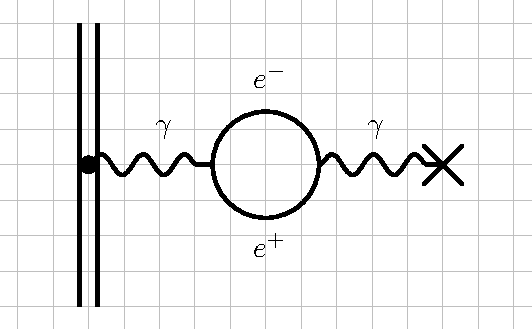
\includegraphics[width=80mm]{Graphs/UehlingLabeled.pdf} 
  \caption{Feynman diagram of the leading-order vacuum polarization contribution to the electron-nucleus interaction. The double lines represent bound states of electrons in the field of the nucleus. Wiggly line is the photon propagator and cross represents the interaction with the field of the nucleus. The double line represents a bound state of the electron and circle a free electron-positron loop.}
  \label{UehlingFig}
\end{figure} 		

Using the charge distribution of~\eqref{NucCharge}, we get the generating integral of the Uehling potential as
\begin{align}
\int e^{-\lambda r}V_{Ue}(r) r^q dr =-\frac{2\alpha^2 Z}{\pi r_0^3}\int e^{-2r_0t}&\big(K_{\lambda,q}(t)+S_{\lambda,q}(t) \nonumber
\\
&-S_{\lambda,q}(-t)\big)\left(1+\frac{1}{2t^2}\right)\frac{\sqrt{1-t^2}}{16 t^5} dt,
\end{align}
and we have defined:
\begin{align}
 S_{\lambda,q}(t) =& (1+2r_0t)\frac{\gamma_q((2t+\lambda)r_0)}{(2t+\lambda)^{q}}, \\ K_{\lambda,q}(t)=&(1+2r_0t+e^{4r_0t}(2r_0t-1))\frac{\Gamma_q((2t+\lambda)r_0)}{(2t+\lambda)^{q}},
\end{align}
where $\gamma_q$ and $\Gamma_g$ are the lower and upper incomplete gamma functions respectively (see Appendix~\ref{app:Gamma}). Closed form of this expression can be found in the limit of small nuclear radius
\begin{align}
I_q^\lambda (r_0) =\int e^{-\lambda r}V_{Ue}(r) r^q dr = -\frac{\alpha^2 Z}{12\pi}(J_{q,1}(\lambda)-\lambda J_{q+1,3}(\lambda)) + O[r_0^2],
\end{align}
where
\begin{align}
J_{q,i}(\lambda) = \Gamma \left(\frac{q}{2}\right)^2\Bigg(\frac{q}{(q+1)(q+3)}&
	{_3F_2}\left[\frac{q}{2},\frac{q+1}{2},\frac{q}{2}+1;\frac{q+5}{2},\frac{i}{2};\frac{\lambda^2}{4}\right] \nonumber
	\\
	&+\frac{2}{q+1}{_3F_2}\left[\frac{q}{2},\frac{q+1}{2},\frac{q}{2};\frac{q+3}{2},\frac{i}{2};\frac{\lambda^2}{4}\right]\Bigg),
\end{align}
and ${}_3F_2$ are the generalized hypergeometric functions.

\begin{table}[]
    \centering
    \begin{tabular}{ccc|cc}
	Element & Z &~$r_{RMS}$ &~$\Delta E^{\rm{Ue}}_{1/Z}$ &~$\Delta E^{\rm{Ue}}_{D-ECM}$ \\
	\hline 
	\hline
	He & 2 & 3.72 $\times 10^{-5}$ & 3.42 $\times 10^{-5}$ & 2.39 $\times 10^{-5}$ \\
	Be & 4 & 4.36 $\times 10^{-5}$ & 2.92 $\times 10^{-4}$ & 2.13 $\times 10^{-4}$ \\
	C & 6 & 4.67 $\times 10^{-5}$ & 9.37 $\times 10^{-4}$ & 6.55 $\times 10^{-4}$ \\
	Ne & 10 & 5.75 $\times 10^{-5}$ & 4.12 $\times 10^{-3}$ & 2.69 $\times 10^{-3}$ \\
	Mg & 12 & 5.78 $\times 10^{-5}$ &  6.89 $\times 10^{-3}$ & 4.64 $\times 10^{-3}$ \\
	Si & 14 & 6.16 $\times 10^{-5}$ &  1.05 $\times 10^{-2}$ & 7.18 $\times 10^{-3}$  \\
	Ar & 18 & 6.33 $\times 10^{-5}$ & 2.10 $\times 10^{-2}$ & 1.45 $\times 10^{-2}$ \\
	Zn & 30 & 7.43 $\times 10^{-5}$ & 8.55 $\times 10^{-4}$ & 5.70 $\times 10^{-4}$ \\
	Kr & 36 & 7.86 $\times 10^{-5}$ & 1.41 $\times 10^{-1}$ & 9.55 $\times 10^{-2}$ \\
	Cd & 48 & 8.47 $\times 10^{-5}$ & 3.13 $\times 10^{-1}$ & 2.12 $\times 10^{-1}$ \\
	\hline
    \end{tabular}
	\caption{Uehling corrections to energy of closed-shell neutral atoms calculated with leading-order~D-ECM compared to the first-order $1/Z$ expansion. Nuclear radii ($r_{RMS}$) taken from~\cite{ANGELI201369}.}
	\label{tab:Uehling}
\end{table}

Once again, we can calculate the resulting correction for any configuration as a finite sum of~$I_q^\lambda (r_0)$ terms with corresponding powers. %(what is the final formula?!)
The results for some neutral atoms are presented in table~\ref{tab:Uehling}.



\chapter{Conclusions and outlook}
\addtocontents{toc}{\contentsline{chapter}{Conclusions and outlook}{\protect\pageref{annotation}}}
\label{ch:Conclusions}

\section{Conclusions}
\label{sec:conclusions}

We have investigated the accuracy and efficiency of the ECM and D-ECM in
describing multi-electron atoms and ions. We have shown, that despite being extremely simple, the analytical approximations produced by the leading-order ECM and D-ECM nevertheless provide accuracy sufficient to obtain correct energy ordering of different electronic configurations, both in ground and excited states. They are also useful in approximating a wide range of other atomic properties. They provide accuracy no worse that $\sim 20\%$ in approximating electronic densities, scattering cross-sections and photoionization cross-sections, and can correctly reproduce the main features, such as electron density maxima coming from the shell structure. Moreover, the accuracy is independent of the number of electrons in an atom, with no more than $\sim 6\%$ error of the total energy for any neutral atom, and significantly better for HCI.

We have also investigated the feasibility of an analytical calculation of second-order corrections. We have shown how the single-electron second-order corrections to energies and first-order corrections to electron densities can be performed analytically in both ECM and D-ECM, by finding generating integrals of the RCGF and RCDGF. These increase the accuracy of the energy calculation to below $\sim 1\%$ for all neutral atoms of the periodic table. We have also numerically evaluated the double-electron corrections to energy, that include the effects of electron-electron correlations, and shown that they correctly reproduce correlation-caused atomic properties, such as electron affinities.

Finally, we have investigated the evaluation of other types of energy corrections within the D-ECM. In particular, those related to the Breit interaction, finite-nuclear-size and vacuum polarization. The accuracy is no worse than $ \sim 5 \%$ in the leading-order approximation in all of the above, even for atoms with a large number of electrons, and can be significantly improved, by evaluating the second-order corrections.

We have shown that ECM is superior to the TF model in approximating both electronic wavefunctions and energies, already in the leading order. It also posses well-defined higher order corrections, that can be used to further increase it's accuracy, and can easily be incorporated, as an initial approximation of other methods, such as the HF method. We therefore expect that the ECM can replace the TF model for all applications were the latter is currently utilised.

We would like to stress, that the introduction of the effective charge
$Z^{*}$, instead of the usage of the nuclear charge $Z$,
i.e. $Z^{*}\neq Z$, is exactly the key idea, that significantly
increases the accuracy of the leading-order approximation,
while rendering the complexity of all calculations low.


Finally, we would like to emphasize that even though our analytical
expressions are sometimes complex, all special functions in the
presented calculations reduce to expressions containing gamma
functions and/or elementary functions only. Therefore, all relevant
evaluations of energies, electron densities and scattering factors can
be performed without any numerical or convergence issues.

\section{Outlook}
			
So far we have calculated ground state energies up to second order and the wave functions up to first order of perturbation theory. However, the ECM and D-ECM might just as easily be extended to higher orders. The third order energy correction is defined as a double series over intermediate states:
\begin{equation}
\Delta E^{(3)}_{\lambda} = \sum_{\sigma_1,\sigma_2 \neq \lambda}\frac{\langle \lambda |\widehat{W}| \sigma_1 \rangle \langle \sigma_1 |\widehat{W}| \sigma_2 \rangle \langle \sigma_2 |\widehat{W}| \lambda \rangle }{(E_\lambda - E_{\sigma_1})(E_\lambda - E_{\sigma_2})} - \langle \lambda |\widehat{W}| \lambda \rangle \sum_{\sigma} \frac{|\langle \lambda |\widehat{W}| \sigma \rangle|^2}{(E_\lambda - E_\sigma)^2}.
\end{equation}
			
This can again be split into a single-electron and a double-electron part and evaluated with a pair of hydrogen Green's functions $G$ or double Green's functions $G^{(2)}$. It is worth investigating, whether the procedure outlined in chapter \ref{ch:IntGreen} allows for a fully analytical calculation of $\Delta E^{(3)}_{\mathrm{single}}$, with multiple convolution integrals over Whitaker functions to express $\Delta E^{(3)}_{\mathrm{double}}$.

On the other hand, the derivatives of Dirac hydrogen-like wavefunctions presented in chapter~\ref{ch:IntGreen}, can be used to derive analytical approximations to atomic properties up to second order in Dirac theory. This will allow for improved accuracy off all results presented in chapters~\ref{ch:Applications} and~\ref{ch:Improvements}, especially in the high-$Z$ examples. Of particular interest is the calculation of transition probabilities outlined in section~\ref{sec:TP}, where the relativistic second-order expressions could be employed to study examples difficult to calculate with other methods, such as the Fe XVII and Ni XIX lines observed in solar corona~\cite{SolarIron}.
			
Furthermore, the leading-order
approximation can easily be modified to include interactions with
external fields. Since the ECM and D-ECM provides the analytic calculation of matrix elements, it is particularly suited for problems, where traditionally it is necessary to use large databases of numerical solutions obtained with indirect optimization procedures such as the HF method or estimational analytical models such as the semi-classical TF model. One such problem may be the time emission of the system, which is periodically driven with a strong field \cite{feranchuk_new_2002}. The Hamiltonian of such system is composed of three parts:
	\begin{equation}
	\widehat{H}(t) = 	\widehat{H}_a + \widehat{H}_{\rm{SF}}(t) + 	\widehat{H}_{\rm{QEM}} ,
	\end{equation}
	where $	\widehat{H}_{\rm{SF}}$ is the strong time-dependent classical field, and $H_{\rm{QEM}}$ is the vacuum electromagnetic field, interaction with which can be treated perturbatively.
	
	Another example might be the process of Bremsstrahlung, which is important for many areas, such as crystallography and approaching it with the HF method becomes inefficient for heavy atoms \cite{PhysRev93788}.
	
		Finally, we are working towards releasing a complete software package, capable of automated and efficient calculation of all observables of interest for many-electron atoms and ions (electron densities, scattering factors, ionization energies etc.). As previously mentioned, a first version capable of performing the calculations in the zeroth order is already available (https://github.com/tupos/effz), and we are working towards extending it to second order.

\begin{appendices}

\chapter{Data tables}

\addtocontents{toc}{\contentsline{chapter}{Appendix: Data tables}{\protect\pageref{annotation}}}

\section{Ground state energies of the first 100 neutral atoms}
\label{app:GroundStates}
  
  In table~\ref{tab:ground_state_energies} we present the values of ground state energies for neutral atoms in the range $Z=1-100$, calculated with leading-order ECM, second-order ECM and leading-order D-ECM, together with the corresponding non-ralativistic $Z^*$ and relativistic $Z_R^*$. For comparison we also provide HF results from ~\cite{Saito2009836} and DHF results from \cite{DESCLAUX1973311} \footnote{In the referenced DHF calculation, the Breit interaction and the nuclear size effect were taken into account and the approximation of the center of gravity of the configuration was used. For the purpose of comparison with D-ECM, we have subtracted the Breit interaction corrections from the reference values, however kept the finite nuclear size correction included, since this effect was not listed explicitly.}.
     
 \begin{table}[]
     \centering \small
     \begin{tabular}{c|cccc|ccc}
    $Z$ &$Z^*$ & $E^{(0)}_\rm{ECM}$ & $E^{(2)}_{\mathrm{single}}$ & $E_{\mathrm{HF}}$ &$Z^*_R$ & $E^{(0)}$_\rm{D-ECM} & $E_{\mathrm{DHF}}$ \\
    \hline \hline
1	&	1	&	-0.5	&	-0.5	&	-0.5	&	1	&	-0.5	&	-0.5	\\
2	&	1.68750	&	-2.84766	&	-2.86100	&	-2.86168	&	1.68749	&	-2.84777	&	-2.86169	\\
3	&	2.54542	&	-7.28906	&	-7.41135	&	-7.43273	&	2.54544	&	-7.28980	&	-7.43301	\\
4	&	3.37160	&	-14.2096	&	-14.5212	&	-14.5730	&	3.37164	&	-14.2122	&	-14.5745	\\
5	&	4.15111	&	-23.6936	&	-24.4115	&	-24.5291	&	4.15118	&	-23.7002	&	-24.5335	\\
6	&	4.91268	&	-36.2016	&	-37.4927	&	-37.6886	&	4.90695	&	-36.1297	&	-37.6704	\\
7	&	5.66045	&	-52.0662	&	-54.1107	&	-54.4009	&	5.64990	&	-51.8947	&	-54.3181	\\
8	&	6.38231	&	-71.2844	&	-74.3812	&	-74.8094	&	6.38076	&	-71.2870	&	-74.8094	\\
9	&	7.09751	&	-94.4525	&	-98.8188	&	-99.4093	&	7.09822	&	-94.5296	&	-99.4778	\\
10	&	7.80729	&	-121.908	&	-127.769	&	-128.547	&	7.80832	&	-122.026	&	-128.656	\\
11	&	8.65613	&	-154.020	&	-160.894	&	-161.859	&	8.65748	&	-154.203	&	-162.028	\\
12	&	9.49720	&	-190.415	&	-198.448	&	-199.615	&	9.49893	&	-190.687	&	-199.867	\\
13	&	10.3161	&	-230.579	&	-240.453	&	-241.877	&	10.3182	&	-230.966	&	-242.241	\\
14	&	11.1294	&	-275.254	&	-287.171	&	-288.854	&	11.1305	&	-275.710	&	-289.344	\\
15	&	11.9377	&	-324.603	&	-338.769	&	-340.719	&	11.9379	&	-325.155	&	-341.345	\\
16	&	12.7366	&	-378.517	&	-395.236	&	-397.505	&	12.7402	&	-379.438	&	-398.409	\\
17	&	13.5314	&	-437.400	&	-456.884	&	-459.482	&	13.5365	&	-438.645	&	-460.704	\\
18	&	14.3222	&	-501.418	&	-523.879	&	-526.818	&	14.3285	&	-503.010	&	-528.397	\\
19	&	15.1910	&	-571.305	&	-595.918	&	-599.165	&	15.1983	&	-573.335	&	-601.178	\\
20	&	16.0556	&	-646.244	&	-673.183	&	-676.758	&	16.0641	&	-648.800	&	-679.224	\\
21	&	16.8063	&	-723.779	&	-755.341	&	-759.736	&	16.8163	&	-726.911	&	-762.887	\\
22	&	17.5526	&	-806.609	&	-843.167	&	-848.406	&	17.5638	&	-810.364	&	-852.242	\\
23	&	18.2939	&	-894.773	&	-936.754	&	-942.884	&	18.3057	&	-899.166	&	-947.515	\\
24	&	18.9135	&	-984.973	&	-1035.65	&	-1043.36	&	19.0435	&	-993.582	&	-1048.82	\\
25	&	19.7636	&	-1087.71	&	-1141.81	&	-1149.87	&	19.7767	&	-1093.63	&	-1156.42	\\
26	&	20.4882	&	-1192.25	&	-1253.26	&	-1262.44	&	20.5065	&	-1199.57	&	-1270.37	\\
27	&	21.2099	&	-1302.72	&	-1371.06	&	-1381.41	&	21.2325	&	-1311.48	&	-1390.84	\\
28	&	21.9279	&	-1419.13	&	-1495.28	&	-1506.87	&	21.9541	&	-1429.38	&	-1517.98	\\
29	&	22.5146	&	-1536.57	&	-1625.17	&	-1638.96	&	22.6724	&	-1553.52	&	-1651.96	\\
30	&	23.3548	&	-1670.43	&	-1763.60	&	-1777.85	&	23.3881	&	-1684.11	&	-1792.94	\\
31	&	24.1826	&	-1809.22	&	-1908.47	&	-1923.26	&	24.2190	&	-1825.05	&	-1940.69	\\
32	&	25.0083	&	-1954.42	&	-2060.00	&	-2075.36	&	25.0473	&	-1972.55	&	-2095.37	\\
33	&	25.8319	&	-2106.13	&	-2218.27	&	-2234.24	&	25.8742	&	-2126.78	&	-2257.11	\\
34	&	26.6516	&	-2264.11	&	-2383.19	&	-2399.87	&	26.6990	&	-2287.85	&	-2426.01	\\
35	&	27.4694	&	-2428.77	&	-2555.03	&	-2572.44	&	27.5214	&	-2455.76	&	-2602.16	\\
36	&	28.2853	&	-2600.19	&	-2733.88	&	-2752.05	&	28.3419	&	-2630.73	&	-2785.70	\\
37	&	29.1585	&	-2780.21	&	-2919.52	&	-2938.36	&	29.2196	&	-2814.78	&	-2976.33	\\
38	&	30.0296	&	-2966.85	&	-3111.99	&	-3131.55	&	30.0955	&	-3005.84	&	-3174.28	\\
39	&	30.8213	&	-3155.02	&	-3310.59	&	-3331.68	&	30.8926	&	-3198.62	&	-3379.60	\\
40	&	31.6110	&	-3350.00	&	-3516.37	&	-3539.00	&	31.6879	&	-3398.57	&	-3592.53	\\
41	&	32.3199	&	-3546.33	&	-3728.64	&	-3753.60	&	32.4810	&	-3605.69	&	-3813.19	\\
42	&	33.1052	&	-3755.01	&	-3949.05	&	-3975.55	&	33.2724	&	-3820.19	&	-4041.76	\\
43	&	33.9674	&	-3976.23	&	-4177.47	&	-4204.79	&	34.0622	&	-4042.09	&	-4278.27	\\
44	&	34.6664	&	-4192.63	&	-4411.72	&	-4441.54	&	34.8505	&	-4271.60	&	-4522.95	\\
45	&	35.4442	&	-4422.14	&	-4654.37	&	-4685.88	&	35.6371	&	-4508.76	&	-4775.81	\\
46	&	36.1379	&	-4652.44	&	-4903.88	&	-4937.92	&	36.4218	&	-4753.60	&	-5037.02	\\
47	&	36.9945	&	-4902.97	&	-5162.74	&	-5197.70	&	37.2051	&	-5006.32	&	-5306.69	\\
48	&	37.8493	&	-5160.83	&	-5429.17	&	-5465.13	&	37.9870	&	-5267.08	&	-5584.77	\\
49	&	38.6966	&	-5424.43	&	-5703.19	&	-5740.17	&	38.8426	&	-5540.99	&	-5871.25	\\
50	&	39.5426	&	-5695.47	&	-5984.91	&	-6022.93	&	39.6968	&	-5823.00	&	-6166.28	\\
51	&	40.3872	&	-5974.00	&	-6274.40	&	-6313.49	&	40.5507	&	-6113.22	&	-6469.96	\\
52	&	41.2295	&	-6259.79	&	-6571.53	&	-6611.78	&	41.4036	&	-6411.79	&	-6782.41	\\
53	&	42.0706	&	-6553.19	&	-6876.53	&	-6917.98	&	42.2552	&	-6718.70	&	-7103.73	\\
54	&	42.9104	&	-6854.26	&	-7189.47	&	-7232.14	&	43.1059	&	-7034.15	&	-7434.02	\\
55	&	43.7925	&	-7165.57	&	-7510.20	&	-7553.93	&	43.9986	&	-7361.18	&	-7773.04	\\
56	&	44.6732	&	-7484.40	&	-7838.70	&	-7883.54	&	44.8903	&	-7696.76	&	-8121.03	\\

    \hline
     \end{tabular}\label{tab:ground_state_energies}
 \end{table} 
  \begin{table}[]
     \centering \small
     \begin{tabular}{c|cccc|ccc}
    $Z$ &$Z^*$ & $E^{(0)}_\rm{ECM}$ & $E^{(2)}_{\mathrm{single}}$ & $E_{\mathrm{HF}}$ &$Z^*_R$ & $E^{(0)}_\rm{D-ECM}$ & $E_{\mathrm{DHF}}$ \\
    \hline \hline
57	&	45.4977	&	-7804.64	&	-8174.35	&	-8221.07	&	45.6404	&	-8026.58	&	-8478.09	\\
58	&	46.2332	&	-8125.81	&	-8516.62	&	-8566.87	&	46.3891	&	-8365.02	&	-8844.56	\\
59	&	46.8783	&	-8447.55	&	-8865.53	&	-8921.18	&	47.1364	&	-8712.08	&	-9220.65	\\
60	&	47.6094	&	-8783.92	&	-9224.48	&	-9283.88	&	47.8818	&	-9067.72	&	-9606.58	\\
61	&	48.3384	&	-9127.99	&	-9591.84	&	-9655.10	&	48.6258	&	-9432.19	&	-10002.5	\\
62	&	49.0657	&	-9479.96	&	-9967.76	&	-10035.0	&	49.3687	&	-9805.72	&	-10408.4	\\
63	&	49.7914	&	-9839.95	&	-10352.3	&	-10423.5	&	50.1103	&	-10188.1	&	-10824.5	\\
64	&	50.6075	&	-10216.4	&	-10747.6	&	-10820.7	&	50.8510	&	-10579.7	&	-11251.0	\\
65	&	51.2340	&	-10582.4	&	-11146.7	&	-11226.6	&	51.5906	&	-10980.7	&	-11688.1	\\
66	&	51.9530	&	-10965.9	&	-11557.2	&	-11641.5	&	52.3290	&	-11391.0	&	-12135.8	\\
67	&	52.6702	&	-11357.4	&	-11976.5	&	-12065.3	&	53.0660	&	-11810.6	&	-12594.2	\\
68	&	53.3856	&	-11757.1	&	-12404.7	&	-12498.2	&	53.8019	&	-12239.8	&	-13063.7	\\
69	&	54.0996	&	-12165.2	&	-12841.9	&	-12940.2	&	54.5370	&	-12678.8	&	-13544.3	\\
70	&	54.8124	&	-12581.8	&	-13288.3	&	-13391.5	&	55.2714	&	-13127.8	&	-14036.1	\\
71	&	55.6210	&	-13017.6	&	-13746.6	&	-13851.8	&	56.1005	&	-13599.6	&	-14539.3	\\
72	&	56.4286	&	-13462.0	&	-14213.9	&	-14321.2	&	56.9293	&	-14081.8	&	-15053.8	\\
73	&	57.2350	&	-13915.1	&	-14690.2	&	-14799.8	&	57.7574	&	-14574.5	&	-15580.0	\\
74	&	58.0403	&	-14376.8	&	-15175.6	&	-15287.5	&	58.5853	&	-15077.9	&	-16117.7	\\
75	&	58.8447	&	-14847.3	&	-15670.3	&	-15784.5	&	59.4133	&	-15592.1	&	-16667.2	\\
76	&	59.6472	&	-15326.2	&	-16173.9	&	-16290.6	&	60.2412	&	-16117.2	&	-17228.8	\\
77	&	60.4487	&	-15813.9	&	-16686.8	&	-16806.1	&	61.0688	&	-16653.3	&	-17802.5	\\
78	&	61.1879	&	-16300.8	&	-17208.2	&	-17331.1	&	61.8960	&	-17200.6	&	-18377.5	\\
79	&	61.9874	&	-16806.4	&	-17739.9	&	-17865.4	&	62.7230	&	-17759.2	&	-18987.1	\\
80	&	62.8473	&	-17330.8	&	-18281.7	&	-18409.0	&	63.5500	&	-18329.3	&	-19598.1	\\
81	&	63.7020	&	-17861.7	&	-18832.7	&	-18961.8	&	64.4318	&	-18920.7	&	-20221.8	\\
82	&	64.5560	&	-18401.7	&	-19393.0	&	-19524.0	&	65.3135	&	-19523.9	&	-20858.3	\\
83	&	65.4092	&	-18950.8	&	-19962.7	&	-20095.6	&	66.1966	&	-20138.7	&	-21507.8	\\
84	&	66.2610	&	-19508.5	&	-20541.5	&	-20676.5	&	67.0798	&	-20765.8	&	-22170.5	\\
85	&	67.1120	&	-20075.4	&	-21129.8	&	-21266.9	&	67.9631	&	-21405.1	&	-22846.7	\\
86	&	67.9623	&	-20651.5	&	-21727.6	&	-21866.8	&	68.8465	&	-22056.9	&	-23528.2	\\
87	&	68.8470	&	-21241.1	&	-22334.9	&	-22475.9	&	69.7641	&	-22727.3	&	-24203.5	\\
88	&	69.7309	&	-21839.6	&	-22951.5	&	-23094.3	&	70.6819	&	-23410.6	&	-24956.6	\\
89	&	70.5707	&	-22437.9	&	-23576.6	&	-23722.2	&	71.4937	&	-24081.0	&	-25687.7	\\
90	&	71.4096	&	-23045.4	&	-24211.2	&	-24359.6	&	72.3057	&	-24764.2	&	-26433.1	\\
91	&	72.1161	&	-23639.5	&	-24850.7	&	-25007.1	&	73.1179	&	-25460.3	&	-27193.3	\\
92	&	72.8875	&	-24254.1	&	-25502.5	&	-25664.3	&	73.9302	&	-26169.3	&	-27968.5	\\
93	&	73.6578	&	-24878.0	&	-26164.2	&	-26331.5	&	74.7427	&	-26891.7	&	-28759.2	\\
94	&	74.3604	&	-25499.2	&	-26833.3	&	-27008.7	&	75.5556	&	-27627.7	&	-29565.3	\\
95	&	75.1286	&	-26141.7	&	-27515.0	&	-27695.9	&	76.3696	&	-28377.3	&	-30387.6	\\
96	&	75.9626	&	-26805.4	&	-28209.0	&	-28392.8	&	77.1841	&	-29141.0	&	-31226.0	\\
97	&	76.7280	&	-27466.1	&	-28910.3	&	-29099.8	&	77.9993	&	-29918.8	&	-32081.0	\\
98	&	77.4251	&	-28124.0	&	-29619.4	&	-29817.4	&	78.8149	&	-30711.0	&	-32953.0	\\
99	&	78.1888	&	-28803.8	&	-30341.2	&	-30545.0	&	79.6310	&	-31517.7	&	-33842.1	\\
100	&	78.9514	&	-29493.1	&	-31073.2	&	-31282.8	&	80.4478	&	-32339.2	&	-34749.1	\\

    \hline
     \end{tabular}
     \caption{Comparison of the values of the total energy of the ground state of neutral atoms between the ECM and the HF method. In order from the left: total nuclear charge $Z$, non-relativistic effective charge $Z^{*}$, leading-order ECM energy ($E^{(0)}_{ECM}$), single-electron second-order ECM energy ($E_{\mathrm{single}}^{(0)}$), numerical solutions of HF equations ($E_{\mathrm{HF}}$)~\cite{Saito2009836}, relativistic effective charge $Z^{*}_R$, leading-order D-ECM energy $E^{(0)}_{D-ECM}$, numerical solutions of DHF equations ($E_{\mathrm{DHF}}$)~\cite{DESCLAUX1973311}.}\label{tab:ground_state_energies}
 \end{table} 
     
 \newpage
 
\section{Excited energies}
\label{app:HCI}

In tables~\ref{tab:Ions} and~\ref{tab:Ions2} we provide the numerical values of excitation energies used for the comparison on figure~\ref{ExcitedPlot}. The results have been obtained by diagonalizing the Hamiltonian in a finite subspace within the leading order D-ECM. See section \ref{sec:Coupling} for details.

\vspace{2cm}

\begin{table}[h!]
\begin{tabular}{cc|ccccc}
  Configuration & $J^{\pm}$ & $Z^{*}$ & $E_{\rm{D-ECM}}$ & CI-DFS
  & $E_{\rm{D-ECM}}/\text{CI-DFS} \cdot 100\%$ \\
  \hline
 \hline 
   $1s^2$ & $0^+$ & 91.80 & -9651.37 & -9651.45 & ~0.001$\%$ \\
  $1s^1 2s^1$ & $1^+$ & 91.92 & 3554.40 & 3554.44 & ~0.001$\%$\\
  $1s^1 2p^1_{1/2}$ & $0^-$  & 91.82 & 3561.28 & 3561.23 & -0.001$\%$\\
   $1s^1 2p^1_{1/2}$ & $1^-$ & 91.82  & 3561.32  & 3561.28 &-0.001$\%$ \\
   $1s^1 2p^1_{3/2}$ & $2^-$ & 91.82 & 3562.41 & 3562.34 & -0.002$\%$ \\
  $1s^1 2s^1$ & $0^+$ & 91.90 & 3723.01  & 3723.01 & 0$\%$  \\
  $1s^1 2p^1_{3/2}$ & $1^-$ & 91.89 & 3724.83  & 3724.77 &-0.002$\%$ \\
  $1s^1 3s^1$ & $1^+$ & 91.89 & 4261.56 & 4261.57 & 0$\%$ \\
  $1s^1 3s^1$ & $0^+$ & 91.83 & 4263.38 & 4263.31 & -0.002$\%$ \\
  \hline
\end{tabular}
  \caption{Comparison of the first few excited energies of he-like uranium ions ${}_{92}$U$^{90+}$,       calculated with a finite subset diagonalization within the leading-order D-ECM, with the results obtained by the configuration-interaction Dirac-Fock-Sturm method~\cite{Tup2003OS} ($\Delta E/E_{\mathrm{DHF}} \cdot 100\%$) and the relative difference between these two in percentages.}
  \label{tab:Ions}
\end{table}

\vspace{2cm}

  \begin{table}[h!]
\begin{tabular}{cc|ccccc}
  Configuration & $J^{\pm}$ & $Z^{*}$ & $E_{\rm{D-ECM}}$ & $E_{\mathrm{exp}}$
  & $E_{\rm{D-ECM}}/E_{\mathrm{exp}} \cdot 100\%$ \\
  \hline
 \hline 
    $1s^22s^2$ & $0^+$ & 25.519 & -812.6 & - & -\\
    $1s^2 2s^12p^1$ & $0^+$ & 25.513 & 1.618 & 1.586 & 2.0$\%$\\
    $1s^2 2s^12p^1_{1/2}$ & $1^-$ & 25.509 & 1.767 & 1.727 & 2.3$\%$\\
    $1s^2 2s^12p^1_{3/2}$ & $2^-$ & 25.509 & 2.201 & 2.150 & 2.3$\%$\\
    $1s^2 2s^12p^1_{3/2}$ & $1^+$ & 25.504 & 3.521 & 3.428 & 2.6$\%$\\
    $1s^2 2p^2_{1/2}$ & $0^+$ & 25.314 & 4.764 & 4.356 & 8.6$\%$\\
    $1s^2 2p^2_{1/2}$ & $1^+$ & 25.319 & 5.092 & 4.680 & 8.1$\%$\\
    $1s^2 2p^1_{1/2} 2p^1_{3/2}$ & $2^+$ & 25.317 & 5.181 & 4.883 & 5.8$\%$\\
    $1s^2 2p^2_{3/2}$ & $2^-$ & 25.321 & 5.846 & 5.487 & 6.1$\%$\\
    $1s^2 2p^2_{3/2}$ & $0^+$ & 25.309 & 6.994 & 6.482 & 7.3$\%$\\
    \hline
\end{tabular}
  \caption{Comparison of the first few excited energies of be-like iron ions ${}_{26}Fe^{22+}$, calculated with a finite subset diagonalization within the leading-order D-ECM, with experimental values taken from the NIST database($E_{\mathrm{exp}}$) and the relative difference between these two in percentages.}
  \label{tab:Ions2}
\end{table}

\newpage
\section{Zeroth order D-ECM densities}
\label{app:zeroDensities}

Here we give the full expressions for electron densities of few-electron atoms and ions calculated within the leading-order D-ECM as a function of $u=2 Z^* r$, using the notation:
\begin{equation}
    h=\sqrt{\frac{\gamma+1}{2}},~~~~~~~~~~~~\gamma=\sqrt{1-(\alpha Z^*)^2}.
\end{equation}
 For the ions with up to 10 electrons we can write compactly:
\begin{equation}
    \rho_{\mathrm{D-ECM}}^{(0)}(r,Z^*) = \frac{4(Z^*)^3}{\Gamma (2 \gamma +1)} \left(4 e^{-u} u^{2 \gamma -2}+\frac{e^{-\frac{u}{2 h}} \left(\frac{u}{2h}\right)^{2 \gamma -2}}{(\gamma +1)^2}Q^{\mathrm{element}}\left(\frac{u}{2h}\right)\right),
\end{equation}
where the polynomials $Q$ are calculated separately for each ion \footnote{Here the atomic symbol refers to the number of electrons. The nuclear charge only influences the value of the effective charge $Z^*$.}:
\begin{subequations}
\begin{align}
     Q^{\mathrm{He}}(x) &= 0 
     \\
     Q^{\mathrm{Li}}(x) &= \frac{1}{4(2 h-1)}x^2-\frac{h+1}{2}x+\frac{h+1}{2} (2 h-1)
     \\
      Q^{\mathrm{Be}}(x) &= \frac{1}{2(2 h-1)}x^2-(h+1)x+(h+1) (2 h-1)
      \\
    Q^{\mathrm{B}}(x) &= \left(\frac{(2 h-1)}{4 (2 \gamma +1)}+\frac{1}{2(2h-1)}\right)x^2-\frac{3h+1}{2}x+1/2(h-\gamma)+(h+1) (2 h-1)
    \\
    Q^{\mathrm{C}}(x) &=\left(\frac{(2 h-1)}{2 (2 \gamma +1)}+\frac{1}{2(2h-1)}\right)x^2-2c x+(h-\gamma)+(h+1) (2 h-1)
    \\
    Q^{\mathrm{N}}(x) &= \left(\frac{3(2 h-1)}{4(2 \gamma +1)}+\frac{1}{2(2h-1)}\right)x^2-\frac{5h-1}{2}x+3/2(h-\gamma)+(h+1) (2 h-1)
    \\
    Q^{\mathrm{O}}(x) &= \left(\frac{(2 h-1)}{(2 \gamma +1)}+\frac{1}{2(2h-1)}\right)x^2-(3h-1)x+2(h-\gamma)+(h+1) (2 h-1)
    \\
    Q^{\mathrm{F}}(x) &= \left(\frac{5(2 h-1)}{4 (2 \gamma +1)}+\frac{1}{2(2h-1)}\right)x^2-\frac{7h-3}{2}x+5/2(h-\gamma)+(h+1) (2 h-1)
    \\
    Q^{\mathrm{Ne}}(x) &= \left(\frac{3(2 h-1)}{2 (2 \gamma +1)}+\frac{1}{2(2h-1)}\right)x^2+2(1-2c)x+3(h-\gamma)+(h+1) (2 h-1)
\end{align}
\end{subequations}

\newpage

\section{First order ECM densities}

Here we give the full expressions for electron densities of few-electron neutral atoms calculated with the ECM up to the first order, using analytic integration of the RCGF. As a function of $u=Z^* r$ we can write:
\begin{align}
\rho^{(1)}(r,Z^*) =& e^{-u}\left(Q_1^{El}(u)+Z^*Q_2^{El}(u)+\xi_1Q_3^{El}(u)+\xi_2Q_4^{El}(u)+\xi_3Q_4^{El}(u)\right) \nonumber
    \\
    &+e^{-2u}\left(Q_6^{El}(u)+Z^*Q_7^{El}(u)+\xi_1Q_8^{El}(u)+\xi_2Q_9^{El}(u)+\xi_3Q_{10}^{El}(u)\right)\nonumber
    \\
    &\mspace{100mu}+e^{-3u}Q_{11}^{El}(u)+e^{-4u}Q_{12}^{El}(u) +e^{-3/2u}Q_{13}^{El}(u),
\end{align}
where the $\xi$ coefficients can be written in terms of the Einstein function (see Appendix) as:
\begin{align*}
\xi_1 &= \text{Ein}(-u)+\log(2),~~~~~~~~~~~~~~~~~~\xi_2 = \text{Ein}(-2u)+\log(3), \\
\xi_3 &= \text{Ein}(-u/2)+\log(3/2),~~~~~~~~~~~~\xi_4 = \text{Ein}(-2u)+\log(2), \\
\xi_5 &= \text{Ein}(-u)+\log(3/2),~~~~~~~~~~~~~~~\xi_6 = \text{Ein}(u/2)-\log(4/3).
\end{align*}
The polynomials $Q(u)$ have to be calculated separately for each atom \footnote{Polynomilas that are not provided are equal to zero.}:
\begin{subequations}
\begin{align}
Q_6^{\text{He}}(u)  &= 3u+\frac{73}{2}u^2-22u^3\\
Q_7^{\text{He}}(u)  &=  16u^2(u-1)\\
Q_8^{\text{He}}(u)  &=  3u^2\\
Q_{12}^{\text{He}}(u)  &=  -u(4u+3);
\end{align}
\end{subequations}
\begin{subequations}
\begin{align}
Q_1^{\text{Li}}(u)  &= -\frac{1027 u^5}{5832}+\frac{31789 u^4}{17496}-\frac{16783 u^3}{4374}+\frac{7045 u^2}{4374}+\frac{298 u}{729}\\
Q_2^{\text{Li}}(u)  &= u^2 \left(\frac{u^3}{8}-u^2+2 u-1\right)\\
Q_4^{\text{Li}}(u)  &= \frac{149}{729} (u-2)^2 u^2\\
Q_6^{\text{Li}}(u)  &=  -\frac{25382 u^3}{729}+\frac{297763 u^2}{4374}+\frac{6859 u}{729}\\
Q_{7}^{\text{Li}}(u)  &= 16 (u-1) u^2 \\
Q_{8}^{\text{Li}}(u)  &= 6 u^2 \\
Q_{9}^{\text{Li}}(u) & = \frac{9344}{729} (u^2) \\
Q_{11}^{\text{Li}}(u) & = -\frac{19 u^4}{18}-\frac{4475 u^3}{729}-\frac{1607 u^2}{81}-\frac{4970 u}{729} \\
Q_{12}^{\text{Li}}(u) & = -3u-4u^2;
\end{align}
\end{subequations}
\begin{subequations}
\begin{align}
Q_1^{\text{Be}}(u)  &=  2 (u-2) u^2 \left(-\frac{168635 u^2}{373248}+\frac{8950903 u}{2239488}-\frac{75323}{93312 u}-\frac{2192035}{1119744}\right)\\
Q_2^{\text{Be}}(u)  &=  \frac{u^2}{4} (u-2) \left(u^2-6 u+4\right)\\
Q_3^{\text{Be}}(u)  &=  \frac{51}{128}(u-2)^2u^2\\
Q_4^{\text{Be}}(u)  &=  \frac{298}{729}(u-2)^2u^2\\
Q_5^{\text{Be}}(u)  &=  0\\
Q_6^{\text{Be}}(u)  &=  -\frac{u^6}{16}-\frac{3 u^5}{16}-\frac{7 u^4}{32}-\frac{4296941 u^3}{93312}+\frac{28064399 u^2}{279936}+\frac{700805 u}{46656}\\
Q_7^{\text{Be}}(u)  &=  16u^2(u-1)\\
Q_8^{\text{Be}}(u)  &=  6u^2\\
Q_9^{\text{Be}}(u)  &=  \frac{18688}{729}u^2\\
Q_{11}^{\text{Be}}(u)  &=  -\frac{19 u^3}{9}+\frac{8950 u^2}{729}+\frac{3214 u}{81}+\frac{9940}{729}\\
Q_{12}^{\text{Be}}(u)  &=  -u\left(4u+3\right);
\end{align}
\end{subequations}
\begin{subequations}
\begin{align}
Q_1^{\text{N}}(u)  &=  -\frac{3656977 u^5}{3359232}+\frac{78700147 u^4}{6718464}-\frac{21160081 u^3}{1119744}+\frac{2453083 u^2}{373248}+\frac{1557457 u}{419904}\\
Q_2^{\text{N}}(u)  &=  \frac{3 u^5}{8}-\frac{5 u^4}{2}+4 u^3-2 u^2\\
Q_3^{\text{N}}(u)  &=  \frac{305 u^4}{128}-\frac{417 u^3}{64}+\frac{417 u^2}{64}\\
Q_4^{\text{N}}(u)  &=  \frac{2071 u^4}{6561}-\frac{1192 u^3}{729}+\frac{1192 u^2}{729}\\
Q_5^{\text{N}}(u)  &=  \frac{1024 u^4}{6561}\\
Q_6^{\text{N}}(u)  &=  -\frac{u^6}{8}-\frac{5 u^5}{8}-\frac{19 u^4}{16}-\frac{22117093 u^3}{279936}+\frac{151975661 u^2}{839808}+\frac{4399141 u}{139968}\\
Q_7^{\text{N}}(u)  &=  16u^2(u-1)\\
Q_8^{\text{N}}(u)  &=  6u^2\\
Q_9^{\text{N}}(u)  &= \frac{132352 u^2}{2187}\\
Q_{10}^{\text{N}}(u)  &=\frac{4096 u^2}{2187} \\
Q_{11}^{\text{N}}(u)  &=  -\frac{19 u^4}{6}-\frac{149503 u^3}{6561}-\frac{532969 u^2}{6561}-\frac{202670 u}{6561}\\
Q_{12}^{\text{N}}(u)  &=  -4 u^2-3 u\\
Q_{13}^{\text{N}}(u)  &= \frac{2048 u^3}{6561}-\frac{4096 u^2}{6561}-\frac{8192 u}{6561};
\end{align}
\end{subequations}
\begin{subequations}
\begin{align}
Q_1^{\text{Ne}}(u) &=  -\frac{810643 u^5}{419904}+\frac{1056691 u^4}{52488}-\frac{87721 u^3}{3456}+\frac{3498481 u^2}{279936}+\frac{390739 u}{52488}\\
Q_2^{\text{Ne}}(u)  &=  \frac{u^5}{2}-3 u^4+4 u^3-2 u^2\\
Q_3^{\text{Ne}}(u)  &=  \frac{83 u^4}{16}-\frac{183 u^3}{16}+\frac{183 u^2}{16}\\
Q_4^{\text{Ne}}(u)  &=  \frac{1460 u^4}{6561}-\frac{1192 u^3}{729}+\frac{1192 u^2}{729}\\
Q_5^{\text{Ne}}(u)  &=  \frac{2048 u^4}{6561}\\
Q_6^{\text{Ne}}(u)  &=  -\frac{u^6}{4}-\frac{7 u^5}{4}-\frac{43 u^4}{8}-\frac{4118851 u^3}{34992}+\frac{1689950 u^2}{6561}+\frac{808279 u}{17496}\\
Q_7^{\text{Ne}}(u)  &=  -16u^2(1-u)\\
Q_8^{\text{Ne}}(u)  &=  6u^2\\
Q_9^{\text{Ne}}(u)  &=  \frac{208640 u^2}{2187}\\
Q_{10}^{\text{Ne}}(u)  &=  \frac{8192 u^2}{2187}\\
Q_{11}^{\text{Ne}}(u)  &=  -\frac{38 u^4}{9}-\frac{218456 u^3}{6561}-\frac{805604 u^2}{6561}-\frac{315880 u}{6561}\\
Q_{12}^{\text{Ne}}(u)  &=  -u(4u+3)\\
Q_{13}^{\text{Ne}}(u)  &=  \frac{4096 u^3}{6561}-\frac{8192 u^2}{6561}-\frac{16384 u}{6561};
\end{align}
\end{subequations}

\chapter{Details of the calculations}

\addtocontents{toc}{\contentsline
{chapter}{Appendix: Details of the calculations}{\protect\pageref{annotation}}}

	This chapter provides more details of the calculations performed throughout the main body of the thesis (in order of appearance).
	
\section{Details of solving the TFD model}

 Section~\ref{sec:TF} describes how the TF model requires a numerical solution of a differential equation known as the TF equation. It has been known since at least 1954 \cite{gilvarry_relativistic_1954} that the relativistic version of this equation can be formally derived in an analogous way by starting from the Dirac Hamiltonian. The result, written in atomic units reads \cite{waber_relativistic_1975}
  \begin{align} 
    \chi''(x) = x^{-1/2}\left(\chi(x) + \frac{Z^}{b c^{2}} \chi'(x) \left(\chi(x) -\frac{1}{2} x \chi'(x)\right)\right)^{3/2}, \label{TFD}
  \end{align}
  where $c$ is the speed of light,
  \begin{equation}
      x = \frac{r}{b},\qquad \qquad b = \left(\frac{9 \pi^2}{128 Z}\right)^{1/3},
  \end{equation}
  and the dimensionless self-consistent potential $\chi(x)$ is related to the self-consistent potential of the TF model as
  \begin{equation}
      \phi(r) = Z \chi(x) - \phi_{0},
  \end{equation}
  with the constant $\phi_{0}$ determined from the normalization condition. For neutral atoms
  $\phi_{0}$ equals zero.
  
  Equation~\eqref{TFD} will be referred to as the TFD equation. Note, that in the non-relativistic limit, i.e., when the speed of light tends to infinity, it reduces to the TF equation~\eqref{TFequation}.

The boundary conditions for the TFD equation in the case of neutral atoms are given by \cite{waber_relativistic_1975}
\begin{align}
  \chi(0) = 1, \qquad \qquad \chi(\infty) = 0. \label{eq:19}
\end{align}
As mentioned in section~\ref{sec:TF}, in order to solve such equation,
one needs to use the shooting method. This means reformulating the
boundary value problem as an initial value one
\begin{align}
  \chi_{0} = 0, \qquad \qquad \chi'(0) = \mu, \label{eq:21}
\end{align}
and seeking a value of $\mu$ that leads to the correct behaviour at infinity. For this purpose the value of $x_c$ needs to be varied from some small value, to a very large one (80 was sufficient for our purposes), and looked for a value of $\mu$ that leads to $\chi(x_c)=0$. The case of the atoms presented in figure~\ref{Rel_rhoPlot}, results in
\begin{align}
  \mu_{\mathrm{Xe}} &= -1.50965873266, \qquad  \qquad \chi_{\mathrm{Xe}}(80) < 10^{-6}, \label{eq:22}
  \\
  \mu_{\mathrm{U}} &= -1.49103044294, \qquad  \qquad \chi_{\mathrm{U}}(80) < 10^{-6}. \label{eq:23}
\end{align}
The high precision required of the $\mu$ values means that this procedure can require significant computation time.

In the case of ions the situation is slightly different. The boundary conditions take the form \cite{marini_relativistic_1981}
\begin{align}
  \chi(0) = 1, \qquad  \qquad  -x_{c}\chi'(x_{c}) = 1 - N/Z, \label{eq:20}
\end{align}
where $N$ is the number of electrons and $x_c$ is the value at which the potential reaches zero: $\chi(x_{c}) = 0$. A similar strategy to neutral atoms can be used here, however one needs to ``shoot'' from
infinity. In this case the boundary value problem is already written
as the initial value one
\begin{align}
  \chi(x_{c}) = 0, \qquad  \qquad \chi'(x_{c}) =
  -\frac{1-N/Z}{x_{c}}, \label{eq:24}
\end{align}
and all that is required, is to vary the value of $x_{c}$, till the value
of $\chi(0)$ becomes one. The two cases of HCI shown in figure~\ref{fig:HCI} give
\begin{align}
  x_{c}
  &= 0.34635, \qquad  \qquad \chi(10^{-6}) \approx 1, \label{eq:25}
  \\
  x_{c}
  &= 0.47890, \qquad  \qquad \chi(10^{-6}) \approx 1. \label{eq:26}
\end{align}

Finally, the density of the atom or ion is expressed through the
self-consistent potential as
  \begin{align}
    \rho(r) = \frac{8\sqrt{2}}{3\pi} \left(\frac{Z
    \chi(x)}{r} - \phi_{0}\right)^{3/2} \left(1 +
    \frac{Z}{b c^{2}}
    \chi'(x) \left(1 - \frac{x
    \chi'(x)}{2\chi(x)}\right)\right)^{3/2}. \label{eq:27}
  \end{align}

\section{Details of the solving the hydrogen atom}
\label{app:hydrogen}

This section provides a more detailed derivation of the hydrogen-like wavefunctions within both Schr\"odinger and Dirac theories.

\subsection{Schr\"odinger equation for hydrogen}

In order to solve the Schr\"odinger equation for the hydrogen atom \eqref{SchSpher} one uses the ansatz
\begin{equation}
	\psi(r,\theta,\varphi) = R(r)Y(\theta,\varphi), \label{SchSplit}
\end{equation}
where both parts are required to be separately normalized
\begin{equation}
	\int R^2 r^2 dr = \int Y^2 \sin(\theta)d\theta d\varphi=1. \label{RYnorm}
\end{equation}
Moreover, since $Y$ is a function on the unit sphere, it also needs to be periodic
\begin{equation}
	Y(\theta,\varphi)=Y(\theta,\varphi+2\pi k)\qquad \text{for} \qquad k \in \mathbb{Z},
\end{equation}
and regular at the poles (as coordinate singularities should not cause physical singularities)
\begin{equation} \label{Ycondition}
	Y(\theta_0,\varphi)=const, \qquad \text{where} \qquad \theta_0 \in\{0,\pi\}.
\end{equation}
Using \eqref{SchSplit} splits \eqref{SchSpher} into the separate radial and angular equations:
\begin{align} \label{Req}
	\frac{d}{dr}\left(r^2 \frac{d R}{d r}\right)+2r(E r+Z)R &= A R, \\
	(1-q^2) \partial_{q}^2 Y - 2q \partial_qY+\frac{1}{1-q^2} \partial^2_{\varphi} Y &= -A Y,\label{Yeq}
\end{align}
where $q = \cos(\theta)$ and $A$ is the separation constant.

Let's first solve the angular equation. It is easy to see that the dependence on $\varphi$ is simple exponential that is traditionally indexed by a parameter $m$
\begin{equation}
    Y(q,\varphi) = e^{i m \varphi}Y(q) \qquad \implies \qquad (1-q^2) \partial^2_q Y-2 q\partial_q Y= \left(\frac{m^2}{q^2-1}-A \right) Y.
\end{equation}
The dependence on $q$ can be found by expanding $Y$ in a power series to obtain a recursion relation
\begin{align}
    &Y(q)=\sum_{i=0}a_iq^i \\
    &(2i^2-m^2-A)a_i-(i+2)(i+1)a_{i+2} +(A-(i-1)(i-2))a_{i-2}=0.
\end{align}
In order for \eqref{Ycondition} to be satisfied the recursion must terminate, which happens whenever $A=l(l+1)$ for some integer $l\geq0$. This makes $Y$ a polynomial in $q$, called associated Legendre polynomial, denoted $P^m_l$ (see Appendix~\ref{app:Legendre}). Finally the angular solutions come out as
\begin{equation}
    Y^m_l(\theta,\varphi) = (-1)^m\sqrt{\frac{(2l+1)}{4\pi}\frac{(l-m)!}{(l+m)!}}P^m_l(\cos(\theta))e^{i m \varphi},
\end{equation}
where the normalization constant is chosen to satisfy \eqref{RYnorm}.

In order to solve the radial equation, one uses the ansatz
\begin{equation}
R(r) = e^{-r\sqrt{-2E}}r^{l-1}g(2\sqrt{-2E}r).
\end{equation}
Plugging in \eqref{Req} it gives
\begin{equation}
    r\partial_{r}^2g+(2l+2-r)\partial_rg+\left(\frac{Z}{\sqrt{-2E}}-l-1\right)g=0,
\end{equation}
where the $A=l(l+1)$ value has been used. One can again expand a series in the powers of $r$ to get
\begin{align}
    &g(r)=\sum_{i=0}a_ir^i \\
    &\left(\frac{Z}{\sqrt{-2E}}-l-1-i\right)a_i+(2l+2+i)(i+1)a_{i+1}=0.
\end{align}
The normalization condition \eqref{RYnorm} requires the recurrence to terminate. This happens when and only when
\begin{equation} \label{RadCondition}
    \frac{Z}{\sqrt{-2E}} = n,
\end{equation} for dome natural number $n>l$. This is the principal quantum number and \eqref{RadCondition} gives the hydrogen spectrum \eqref{SchEnergy}. In that case the function $g$ is a polynomial, called Laguerre polynomial, defined by \eqref{Laguerre}. Finally the bound states come out as
\begin{equation} %Check this
	R_{n,l,Z}(r)=\sqrt{\frac{(n+l)!}{(n-l-1)!}}\frac{Z^{1/2}}{2 r n}\left(\frac{2 Z}{n} r\right)^l L_{n-l-1}^{2l+1}\left(\frac{2Z}{n}r \right),
\end{equation}

When the energy is not at a resonant value given by \eqref{RadCondition}, the radial equation has two general solutions:
\begin{subeqeations}
\begin{align} \label{generalR}
   	R_{\nu,l,Z}&=\sqrt{\frac{(\nu+l)!}{(\nu-l-1)!}}\frac{\sqrt{Z}}{2 r \nu}M \left[\nu,l+\frac{1}{2},\frac{2Z}{\nu}r \right] \\
	U_{\nu,l,Z}&=\sqrt{\frac{(\nu+l)!}{(\nu-l-1)!}}\frac{\sqrt{Z}}{2 r \nu}W \left[\nu,l+\frac{1}{2},\frac{2Z}{\nu}r \right],
\end{align}
\end{subeqeations}
where $\nu = Z/\sqrt{-2E}$ and the functions $M$ and $W$ are the two kinds of Whittaker functions (see Appendix~\ref{app:Whittaker}).

On the other hand, the free states, that is states with $E>0$, are required to satisfy $R(\infty) = e^{i k r}$ instead of are given by $\nu = -i/k$ and $E=k^2/2$. Note that this produces a discrete spectrum for $E<0$ and a continuous one for $E>0$, as expected.

\subsection{Dirac equation for hydrogen}

The relativistic case can be approached in an analogous way. Requiring the wavefunctions to be eigenvactors of the total momentum operator and the spin operator, leads to the ansatz~\cite{flugge_practical_1971}
\begin{equation} \label{Diracwave}
	\psi(r) = \left(\begin{matrix}g_{n_k,\kappa}(r) \Omega_{\kappa,m_j}(\theta,\varphi) \\ f_{n_k,\kappa}(r) \Omega_{-\kappa,m_j}(\theta,\varphi)\end{matrix}\right),
\end{equation}
This splits the Dirac equation for hydrogen into the radial and angular equations. The angular equation does not admit a simple form, but it can be solved, by simply using the properties of the angular momentum operator~\cite{flugge_practical_1971}. The result comes out as
\begin{align}
  \Omega_{\kappa,m}
  (\theta,\varphi)= \left(
    \begin{array}{c}
      \sqrt{\frac{1}{2} - \frac{m}{2\kappa+1}}
      Y_\kappa^{m-1/2}(\theta,\varphi)
      \\
      -\sqrt{\frac{1}{2} + \frac{m}{2\kappa+1}}
      Y_\kappa^{m+1/2}(\theta,\varphi)
    \end{array}
  \right), \label{eq:29}
\end{align}
where $\kappa$ is the relativistic angular quantum number defined by~\eqref{eq:kappa}.

The radial wavefunctions meanwhile satisfy the system of coupled equations:
\begin{subeqeations}
    \begin{align}
	\partial_r g+\frac{1+\kappa}{r} g - i \left(\alpha \left(E+\frac{z}{r}\right)+c\right)f &=0 \\
\partial_r f+\frac{1-\kappa}{r} f - i \left(\alpha \left(E+\frac{z}{r}\right)+c\right)g &=0 
\end{align}
\end{subeqeations}
Plugging one into the other gives an equation of the same class as~\eqref{Req} which means that $f$ and $g$ can be written as combinations of the non-relativistic radial solutions. Using the notation of section~\eqref{sec:Dirachydro} the result becomes
\begin{align} \label{fullRelR}
\left(\begin{matrix}g_{n,\kappa,z}(r)  \\ f_{n,\kappa,z}(r)\end{matrix}\right) = N_{n,\kappa}\Big[s \left(\begin{matrix}\sqrt{\kappa+\gamma}  \\-\sqrt{\kappa-\gamma}\end{matrix}\right) &R_{n_k+\gamma,\gamma,\varepsilon z}(r) \nonumber \\
-&i \rho \left(\begin{matrix}\sqrt{\gamma-\kappa}  \\\sqrt{\kappa+\gamma}\end{matrix}\right) R_{n_k + \gamma,\gamma-1,\varepsilon z}(r)\Big],
\end{align}
where the normalization constant comes out, as
\begin{align*}
  N_{n,\kappa}=\cfrac{1}{\sqrt{\left(\cfrac{2 \gamma}{\kappa \varepsilon} -1 \right)s^2+\rho^2}},
\end{align*}
where $E_{n,\kappa}$ is the energy of a bound state given by~\eqref{DiracEnergy}.

It is worth mentioning here that for the convenience of presentation, the Dirac
  wavefunctions have been expressed through the Schr\"odinger wavefunctions and not through more
  commonly used hypergeometric functions~\cite{AS}. However, our definition in~\eqref{fullRelR} is completely equivalent to other representations commonly used in literature~\cite{flugge_practical_1971}.

Furthermore, the relation between Schr\"odinger and Dirac wavefunctions given by~\eqref{fullRelR} is also valid for arbitrary energies, with $n \rightarrow \nu$ and can express the second solution of the radial equation under $R(r) \rightarrow U(r)$, which is particularly useful when dealing with the Coulomb Green's functions, allowing for a uniform treatment of RCGF and RCDGF.

\section{Details of the leading-order calculation}
\label{app:ECM}

As shown in chapter~\ref{ch:ECM} the leading-order calculation reduces to evaluating two kinds of radial integrals:
\begin{align}
    T_{\lambda} =& \int \frac{|\psi_{\lambda}(r)|^2}{r} dr,
    \\
       T^{\lambda_3,\lambda_4}_{\lambda_1,\lambda_2}(k) =& \int \psi_{\lambda_1}(r_1)^* \psi_{\lambda_2}^*(r_2) \psi_{\lambda_3}(r_1) \psi_{\lambda_4}(r_2) \frac{\min[r_1,r_2]^k}{\max[r_1,r_2]^{k+1}} r_1^2 r_2^2 dr_1 dr_2,
\end{align}
with the angular part handled by the closed form formula~\eqref{3jInt}.

In order to evaluate $T_{\lambda}$, note that for any natural number $a$, we have:
\begin{subequations}
\begin{align}
  \int M_{a+b,b-1/2}(r) M_{a+b,b-1/2}(r) \frac{dr}{r} &= \frac{\Gamma(2b)^2 (a)!}{\Gamma(a+2b)}, 
  \\
  \int M_{a+b,b+1/2}(r) M_{a+b,b+1/2}(r) \frac{dr}{r} &= \frac{\Gamma(2b+2)^2 (a-1)!}{\Gamma(a+2b+1)},
  \\
  \int M_{a+b,b+1/2}(r) M_{a+b,b-1/2}(r) \frac{dr}{r} &= \frac{\Gamma(2b)\Gamma(2b+2) (a)!}{\Gamma(a+2b+1)},
  \end{align}    
\end{subequations}
and using the general formula~\eqref{generalR} we get in the non-relativistic case
\begin{equation}
 \label{Aformula}
   T_{\lambda} = \frac{Z^*}{n^2}.
\end{equation}
Similarly, using~\eqref{fullRelR} we get the relativistic case, as
\begin{equation}%Intermediate step?
    T_{\lambda} = \left(\frac{(\alpha Z^*)^2}{\gamma}+n_k\right)\left(\frac{\varepsilon}{n_k}\right),
\end{equation}

For the purpose of subset diagonalization the off-diagonal $T_{\lambda}$ integrals are also needed. In particular
\begin{equation}
     T_{\lambda_1,\lambda_2} =& \int \frac{\psi_{\lambda_1}(r)^*\psi_{\lambda_2}(r)}{r} dr,
\end{equation}
can be evaluated using:
\begin{subeqeation}
\begin{align}
  \int M_{a_1+b,b-1/2}&(k_1r) M_{a_2+b,b-1/2}(k_2r) \frac{dr}{r} \nonumber
  \\
  &= \Gamma(2b) x^{b}y^{a_1+a_2+2b}{}_2F_1[-a_1,-a_2,2b,-x], 
  \\
  \int M_{a_1+b,b+1/2}&(k_1r) M_{a_2+b,b+1/2}(k_2r) \frac{dr}{r} \nonumber
  \\
  &= \Gamma(2b+2) x^{b+1}y^{a_1+a_2+2b}{}_2F_1[1-a_1,1-a_2,2b+2,-x],
 \end{align}
\end{subeqeation}
where
\begin{equation}
    x=\frac{4k_1k_2}{(k_1-k_2)^2}\qquad\qquad y=\frac{|k_1-k_2|}{k_1+k_2},
\end{equation}
and ${}_2F_1$ is the Gauss hypergeometric function.

Furthermore, in order to evaluate $T_{\nu_2,\nu_4}^{\nu_1,\nu_3}$, we
employ the integral
\begin{align}
  \int_0^\infty e^{-\lambda r - \lambda' r'} r^q
    {r'}^{q'} r_{<}^{p} r_{>}^{p'} dr dr' =& \int_0^\infty \int_r^\infty e^{-\lambda r - \lambda' r'} r^{q+p} {r'}^{q'+p'} dr' dr\nonumber
    \\
     &+ \int_0^\infty \int_{r'}^\infty
    e^{-\lambda' r' - \lambda r} r^{q+p'} {r'}^{q'+p} dr dr'
    \nonumber
  \\
  &~~~~=
    u_{q+p+1}^{q'+p'+1}(\lambda',\lambda) +
    u_{q'+p+1}^{q+p'+1}(\lambda,\lambda'). \label{eq:62}
\end{align}
where $u_a^b(\lambda,\lambda')$ is the generating integral of the Heaviside theta function, and as such can be evaluated using~\eqref{uGen} and~\eqref{uInteger}. Since in the case of bound states, the Whittaker functions can be expanded as a product of an exponential and a polynomial, the required integral becomes
  \begin{align}
   & \int
    M_{a_1+b_1,b_1-1/2}(q_1 r) M_{a_2+b_2,b_2-1/2}(q_2 r) \nonumber
    \\
      &\mspace{50mu}\times M_{a_3+b_3,b_3-1/2}(q_3 r')M_{a_4+b_4,b_4-1/2}(q_4 r')
      \frac{r_<^l}{r_>^{l+1}} dr dr' \nonumber
    \\
    &\mspace{50mu}=\sum_{i_1=0}^{a_1} \sum_{i_2=0}^{a_2} \sum_{i_3=0}^{a_3}
      \sum_{i_4=0}^{a_4} T_{\vec{a},\vec{b},\vec{q}}(\vec{i})
      \Big(u_{i_1+i_2+b_1+b_2+l+1}^{i_3+i_4+b_3+b_4-l}
      \left(\frac{q_3+q_4}{2},\frac{q_1+q_2}{2}\right) \nonumber
      \\
      &\mspace{250mu}+ u_{i_3+i_4+b_3+b_4+l+1}^{i_1+i_2+b_1+b_2-l}
      \left(\frac{q_1+q_2}{2},\frac{q_3+q_4}{2}\right)\Big),
  \end{align}
  where
  \begin{align*}
    T_{\vec{a},\vec{b},\vec{q}}(\vec{i}) =
    \prod_{k=1}^4
    \frac{\Gamma(2b_k)}{\Gamma(2b_k+i_k)}
    (-1)^{i_k}q_k^{b_k+i_k}.
  \end{align*}
  The bold $\vec a$,
  $\vec b$, $\vec q$ and $\vec i$ are lists of four values, i. e.,
  $\vec a = \{a_{1}, a_{2}, a_{3}, a_{4}\}$ with similar expressions
  for $\vec b$, $\vec q$ and~$\vec i$.
	
 \section{Details of the scattering factors calculation}
  \label{app:scatter}
  
 This section presents the calculation of atomic scattering factors, as Fourier
    transforms of electronic density
  \begin{align}
    f_{n_r,\kappa}(q,Z^*) = \int \rho_{n_r,\kappa} (r,Z^*) e^{i
    \vec{q} \cdot \vec{r}} d \vec{r}. \label{eq:40}
  \end{align}
  Integrating out the angular dependence in~\eqref{densityFormula}, we get the
  radial density as
  \begin{align}
    \rho (r,Z^*) = \sum_{\lambda}
    |g_{\lambda}(r,Z^*)|^2+|f_{\lambda}(r,Z^*)|^2, \label{eq:39}
  \end{align}
  
  Now, expanding the Dirac wavefunctions, as exponentials and polynomilas and using \cite{gradstejn_table_2009}
  \begin{align}
    \int e^{-\lambda r}r^{n-2} e^{i \vec{q} \cdot \vec{r}} d\vec{r} =
    4\pi \Gamma(n) \frac{\sin(n
    \tan^{-1}(\frac{q}{\lambda}))}{\sqrt{(\lambda^2+q^2)^n}},
    \label{eq:42}
  \end{align}
  we get
  \begin{align}
    f_{n_r,\kappa}(q,Z^*)=& (N(2\gamma+1)\Gamma(2\gamma))^2 \nonumber
    \\
     &\times \left(
    2\kappa (\kappa-\gamma) n_r^2\sigma_1 + 4(\kappa-\gamma) \rho n_r
    \sigma_2 +
    \frac{2\kappa}{\kappa+\gamma}\rho^2\sigma_3\right), \label{eq:41}
  \end{align}
  where
  \begin{align*}
    \sigma_{1}
    &= \sum_{\substack{i=1\\j=1}}^{n_r} {{n_r-1}\choose{i-1}}
    {{n_r-1}\choose{j-1}}
    \frac{\Gamma(i+j+2\gamma)}{\Gamma(2\gamma+i+1)!
    \Gamma(2\gamma+j+1)!} \xi_{i,j}(q,Z^*),
    \\
    \sigma_{2}
    &= \sum_{\substack{i=1\\j=0}}^{n_r} {{n_r-1}\choose{i-1}}
    {{n_r}\choose{j}} \frac{\Gamma(i+j+2\gamma)}{\Gamma(2\gamma+i+1)!
    \Gamma(2\gamma+j)!} \xi_{i,j}(q,Z^*),
    \\
    \sigma_{3}
    &= \sum_{\substack{i=0\\j=0}}^{n_r} {{n_r}\choose{i}}
    {{n_r}\choose{j}}
    \frac{\Gamma(i+j+2\gamma)}{\Gamma(2\gamma+i)!\Gamma(2\gamma+j)!}
    \xi_{i,j}(q,Z^*),
    \\
    \xi_{i,j}(q,Z^*)
    &= \frac{(-1)^{i+j}}{q} \sin\left((i+j+2\gamma)
      \tan^{-1}\left(\frac{q}{2\chi Z^*}\right)\right) \left(\frac{2
      \chi Z^*}{\sqrt{(2\chi Z^*)^2+q^2}}\right)^{i+j+2\gamma}.
  \end{align*}
  
  \section{Details of the photoionization calculation}
  \label{app:photo}
  
  This section presents the details of the calculation of
  Eq.~\eqref{PICformula}.  Within the framework of the D-ECM, $\psi_f$ is described as a free-state solution to the Dirac equation, with energy $E$, momentum $p$ and efffective charge $Z^*$. It can be written compactly, as \cite{PhysRev.134.A898}
  \begin{align}
    \psi_{\rm{free}} =& \left(\begin{matrix}
        g_{p,\kappa'} (r,Z^*)~~ \Omega_{\kappa',m'}
        \\
        f_{p,\kappa'} (r,Z^*)~~\Omega_{-\kappa',m'}
      \end{matrix}\right) \nonumber
      \\
      &= \frac{1}{2\sqrt{p r}}
    \frac{|\Gamma(1+\gamma+i \nu)|}{\Gamma(2\gamma+1)}
    \left(\begin{matrix}\sqrt{1/\varepsilon+1} \text{Im}(\Psi (r,Z^*))~~
        \Omega_{\kappa',m'}
        \\
        \sqrt{1/\varepsilon-1} \text{Re}(\Psi
        (r,Z^*))~~\Omega_{-\kappa',m'} \end{matrix}\right),
  \end{align}
  with $\nu = Z^* \varepsilon/p$ and
  \begin{equation}
    \Psi (r,Z^*) =(1+i)\sqrt{\frac{\kappa - i Z^*/p}{\gamma-i \nu}}
    e^{\pi/2 (\nu+i \gamma)} M_{1/2+i \nu,\gamma}(-2i p r).
  \end{equation}
  
  Using the orthogonality
  \begin{equation}
    \int \xi_{\kappa,m}\xi_{\kappa',m'} d\Omega =
    \frac{1}{2}\delta_{\kappa,\kappa'}\delta_{m,m'},
  \end{equation}
  equation~\eqref{PICformula} can be integrated to obtain the total
  photoionization cross section, as
  \begin{equation}
    \sigma_{\mathrm{tot}} = \frac{\alpha p \varepsilon}{k} 4\pi
    \sum_{\kappa',m'} \left|\vec{J}\right|^2,
  \end{equation}
  where
  \begin{equation}
    \vec{J} = 
    \int\left(\begin{matrix}
        g_{p,\kappa'}(r,Z^*)~~
        \Omega_{\kappa',m'}
        \\
        f_{p,\kappa'}(r,Z^*)~~\Omega_{-\kappa',m'}
      \end{matrix}\right)^{\dagger}\left(\begin{matrix}
        0&&\vec{\sigma}
        \\
        \vec{\sigma}&&0
      \end{matrix}\right)\left(\begin{matrix}
        g_{n,\kappa}(r,Z^*)~~ \Omega_{\kappa,m}
        \\
        f_{n,\kappa}(r,Z^*)~~\Omega_{-\kappa,m}
      \end{matrix}\right) d\vec{r},
  \end{equation}
  with different Pauli matrices {$\sigma$}corresponding to different
  polarization directions. Directing the photon momentum along the
  {\it{z}} axis of our coordinate system
  ($\vec{e}^1, \vec{e}^2, \vec{k}$) and summing over photon
  polarization states, we get~\cite{lifshitz1974relativistic}
  \begin{equation}
    \sum_{i,j,s} J^*_i J_j e_i^s e_j^s
    =\frac{1}{2}\left(|\vec{J}|^2-\frac{(\vec{J} \cdot
        \vec{k})(\vec{J^*} \cdot \vec{k})}{k^2}\right) =
    \frac{|J_x|^2+|J_y|^2}{2} = |J_x|^2,
  \end{equation}
  where in the last step the symmetry of the
  remaining two directions has been exploited. This means that the total
  photoionization cross-section can be calculated as
  \begin{align}
    \sigma_{\mathrm{tot}} =& \frac{\alpha p \varepsilon}{k} 4\pi
    \sum_{\kappa',m'} \Bigg|\int\left(\begin{matrix}
          g_{p,\kappa'}(r,Z^*)~~ \Omega_{\kappa',m'}
          \\
          f_{p,\kappa'}(r,Z^*)~~\Omega_{-\kappa',m'}
        \end{matrix}\right)^{\dagger}
        \nonumber
        \\
        &\mspace{180mu}\times\left(\begin{matrix}
          0&&\sigma_1
          \\
          \sigma_1&&0
        \end{matrix}\right)\left(\begin{matrix}
          g_{n,\kappa}(r,Z^*)~~
          \Omega_{\kappa,m}\\f_{n,\kappa}(r,Z^*)~~\Omega_{-\kappa,m}
        \end{matrix}\right)d\vec{r}\Bigg|^2.
  \end{align}
  
  Now, using the orthogonality of spherical harmonics, one can
  see that
  \begin{equation}
    \int\Omega^{\dagger}_{\kappa',m'}\sigma_1\Omega_{\kappa,m}
    d\Omega=(\delta_{\kappa',\kappa} + \delta_{\kappa',-1-\kappa})
    (\delta_{m',m+1} C_{\kappa',m'} D_{\kappa,m} + \delta_{m',m-1}
    D_{\kappa',m'}C_{\kappa,m}),
  \end{equation}
  where $C_{\kappa,m}= \sqrt{\frac{1}{2} - \frac{m}{2\kappa+1}}$ and
  $D_{\kappa,m} = \sqrt{\frac{1}{2} + \frac{m}{2\kappa+1}}$ are
  numerical coefficients of spherical harmonics, see
  Eq.~\eqref{eq:29}. This gives us
  \begin{align}
    &\left|\int\left(\begin{matrix}
          g_{p,\kappa'}(r,Z^*)~~ \Omega_{\kappa',m'}
          \\
          f_{p,\kappa'}(r,Z^*)~~\Omega_{-\kappa',m'}
        \end{matrix}\right)^{\dagger}\left(\begin{matrix}
          0&&\sigma_1
          \\
          \sigma_1&&0
        \end{matrix}\right)\left(\begin{matrix}
          g_{n,\kappa}(r,Z^*)~~ \Omega_{\kappa,m}
          \\
          f_{n,\kappa}(r,Z^*)~~\Omega_{-\kappa,m}
        \end{matrix}\right)d\vec{r}\right| \nonumber 
    \\
    &~~=J_{\kappa'}(\delta_{\kappa',-\kappa} +
      \delta_{\kappa',-1+\kappa}) (\delta_{\kappa'm',m+1}
      C_{\kappa',m'} D_{-\kappa,m} + \delta_{m',m-1} D_{\kappa',m'}
      C_{-\kappa,m} \nonumber)
    \\
    &~~+I_{-\kappa'}(\delta_{-\kappa'\kappa} +
      \delta_{-\kappa',-1-\kappa}) (\delta_{m',m+1} C_{-\kappa',m'}
      D_{\kappa,m} + \delta_{m',m-1} D_{-\kappa',m'} C_{\kappa,m}),
  \end{align}
  where the radial integrals read:
  \begin{equation}
    \left(\begin{matrix}
        I_{\kappa'}
        \\
        J_{\kappa'}
      \end{matrix}\right)=\int \left(\begin{matrix}
        g_{n,\kappa}(r,Z^*)~~ f^*_{p,\kappa'}(r,Z^*)
        \\
        f_{n,\kappa}(r,Z^*)~~g^*_{p,\kappa'}(r,Z^*)
      \end{matrix}\right) r^2dr
  \end{equation}
  and can always be performed analytically within the ECM. Finally, the result comes out as
  \begin{align}\label{eq:sigmaTot}
    \sigma_{\mathrm{tot}} =& \frac{\alpha p \varepsilon}{k} 4\pi
    \Big[\left|I_{-\kappa}\right|^2 A_{\kappa,\kappa} +
    \left|J_{-\kappa}\right|^2 A_{-\kappa,-\kappa} \nonumber
    \\
    &+2\text{Re}(I_{-\kappa}^* J_{-\kappa}B_\kappa) +
    \left|I_{\kappa+1}\right|^2 A_{-\kappa-1,\kappa} +
    \left|J_{\kappa-1} \right|^2A_{\kappa-1,-\kappa}\Big],
  \end{align}
  where:
  \begin{align}
    &A_{\kappa,\kappa'} = \left|C_{\kappa,m+1}D_{\kappa',m}\right|^2
      + \left|C_{\kappa',m} D_{\kappa,m-1}\right|^2 
    \\
    &B_\kappa = C_{\kappa,m+1} D_{\kappa,m} C_{-\kappa,m+1}
      D_{-\kappa,m} + C_{\kappa,m} D_{\kappa,m-1} C_{-\kappa,m}
      D_{-\kappa,m-1}.
  \end{align}
  
  For the purpose of estimating the relevance of relativistic
  corrections, one can take the low $p$ limit in \eqref{eq:sigmaTot} and
  average over the $m$ quantum number to obtain a non-relativistic
  formula
  \begin{align}
    \sigma_{\mathrm{tot}}=&\frac{4\pi^2 \alpha (Z^*)^2}{3 p \omega
      (2l+1)} \Bigg(\frac{1}{l}\left|\int R_{n,l,Z^*}(r)R_{p,l-1,Z^*}(r)
        r^2dr\right|^2 \\
        &\mspace{100mu}+ \frac{1}{l+1}\left| \int R_{n,l,Z^*}(r)
        R_{p,l+1,Z^*}(r)r^2dr\right|^2\Bigg),
  \end{align}
  or equivalently
  \begin{align}
    \sigma_{\mathrm{tot}}=&\frac{4\pi^2 \alpha}{3 p (2l+1)}
    \left(1+\frac{E-E^0}{\omega}\right)\Bigg(l \left|\int
        R_{n,l,z}(r) R_{p,l-1,z}(r)r^3dr\right|^2 \\
        &\mspace{200mu}+ (l+1) \left|\int
        R_{n,l,z}(r) R_{p,l+1,z}(r)r^3dr\right|^2\Bigg),
  \end{align}
  where $E$ and $E^0$ are the ionization energy and the \changeR{leading}-order
  energy of the bound state wave function. For the case of $E=E^0$ it
  reduces to the standard formula \cite{YEH19851}.

\chapter{Special functions}

\addtocontents{toc}{\contentsline
{chapter}{Appendix: Special functions}{\protect\pageref{annotation}}}

	This chapter provides formulas defining some of the special functions used throughout this thesis, as well as relations between them.
	
\section{Legendre polynomials}
\label{app:Legendre}

Despite the name, Legendre polynomials $P_n^m(x)$ are in fact polynomials only for odd values of $m$. For even $m$ the involve square roots. They can be defined, as
\begin{equation}
    P_n^m(x) = (1-x)^m\left(\sqrt{1-x^2}\right)^{m}\sum_{i=m}^n \frac{(n+i)!}{(n-i)!}\frac{\left(\frac{z-1}{2}\right)^i}{(i-m)!i!}.
\end{equation}
Since they appear in the study of angular momentum, it is useful to write $x=\cos(\theta)$, to get
\begin{equation}
    P_n^m(\cos(\theta)) = (2\sin(\theta))^{m}\sum_{i=m}^n \frac{(n+i)!}{(n-i)!}\frac{(-1)^i}{i!}\frac{\left(\sin(\frac{\theta}{2})\right)^{2i+2m}}{(i-m)!}.
\end{equation}
For an explicit form of the first few Laguerre's, see~\ref{app:Harmonics}.

Legendre polynomials are orthogonal for a fixed value of $m$, as
\begin{equation}
    \int_{-1}^1P_n^m(x)P_k^m(x) dx = \frac{2}{2n+1} \frac{(n+m)!}{(n-m)!} \delta_{nk},
\end{equation}
and for a fixed value of $n$, as
\begin{equation}
    \int_{-1}^1P_n^m(x)P_n^k(x) \frac{dx}{1-x^2} = \frac{1}{m} \frac{(n+m)!}{(n-m)!} \delta_{mk}.
\end{equation}

\section{Laguerre polynomials}
\label{app:Laguerre}

Laguerre polynomials are polynomials defined, as
\begin{equation}
    L_n^m(x) =\sum_{i=m}^n \frac{(n+m)!}{(n-i)!(m+i)!}\frac{(-x)^i}{i!}.
\end{equation}
The first few are explicitly, given by:
\begin{subequations}
\begin{align}
    L_0^m(x)&=1, \\
    L_1^m(x)&=1+m-x, \\
    L_2^m(x)&=\frac{(1+m)(2+m)}{2}-(m+2)x+\frac{x^2}{2}, \\
    L_3^m(x)&=\frac{(1+m)(2+m)(3+m)}{6}-\frac{(2+m)(3+m)}{2}x+\frac{m+3}{2}x^2-\frac{x^3}{2}.
\end{align}
\end{subequations}
Laguerre polynomials are orthogonal for a fixed value of $m$ with a weight of $e^{-x}x^m$, as
\begin{equation}
    \int_{0}^\infty e^{-x}x^m L_n^m(x)L_k^m(x) dx = \frac{(n+m)!}{n!} \delta_{nk}.
\end{equation}
Since they appear in the representation of radial hydrogen wavefunctions, it is useful to have a closed form of the generating integral of a product of two $L_{n}^m(x)$ with a fixed $m$. Accoring to~\cite{LandauQM}, we have
\begin{align}
    \int_{0}^\infty e^{-\lambda x}x^{m} L_{n_1}^m(k_1x)L_{n_2}^m&(k_2x) dx = \frac{(n_1+m)!}{n_1!t_1^{n_1}} \frac{(n_2+m)!}{n_2!t_2^{n_2}} \nonumber
    \\
    &\times \lambda^{-m-1}{}_2\widetilde{F}_1\left[-n_1,-n_2,m+1,(t_1-1)(t_2-1)\right],
\end{align}
where ${}_2\widetilde{F}_1$ is the regularized Gauss hypergeometric function~\cite{AS}, and I have defined
\begin{equation}
    t_1 = \frac{\lambda}{\lambda-k_1}, \qquad \qquad t_2 = \frac{\lambda}{\lambda-k_2}.
\end{equation}

\section{Spherical harmonics}
\label{app:Harmonics}

Spherical can be written in terms of the Laguerre polynomials, as
\begin{equation}
    Y^m_l(\theta,\varphi) = (-1)^m\sqrt{\frac{(2l+1)}{4\pi}\frac{(l-m)!}{(l+m)!}}P^m_l(\cos(\theta))e^{i m \varphi}.
\end{equation}
\begin{subequations}
Their properties have already been described in the main body of the thesis, so here I only present the explicit form of the first few spherical harmonics:
\begin{align}
Y_0^0(x)&=\frac{1}{\sqrt{4\pi}} \\
Y_1^{-1}(\theta,\varphi)&=\sqrt{\frac{3}{8\pi}}\sin(\theta)e^{-i\varphi}, \\
Y_1^{0}(\theta,\varphi)&=\sqrt{\frac{3}{4\pi}}\cos(\theta), \\
Y_1^{1}(\theta,\varphi)&=-\sqrt{\frac{3}{8\pi}}\sin(\theta)e^{-i\varphi}, \\
Y_2^{-2}(\theta,\varphi)&=\sqrt{\frac{15}{128\pi}}(1-\cos(2\theta))e^{-2i\varphi},\\
Y_2^{-1}(\theta,\varphi)&=\sqrt{\frac{15}{32\pi}}\sin(2\theta)e^{-i\varphi}, \\ Y_2^{0}(\theta,\varphi)&=\sqrt{\frac{5}{64\pi}}(3\cos(2\theta)+1), \\  Y_2^{-1}(\theta,\varphi)&=\sqrt{\frac{15}{32\pi}}\sin(2\theta)e^{-i\varphi}, \\ Y_2^{2}(\theta,\varphi)&=\sqrt{\frac{15}{128\pi}}(1-\cos(2\theta))e^{-2i\varphi}.
\end{align}
\end{subequations}

\section{Whittaker functions}
\label{app:Whittaker}

Whitteker functions are defined as solutions of the Whittaker equation, which can be written as~\cite{bams}
\begin{equation}
    \partial_x^2 y + \left(\frac{\lambda(1-\lambda)}{x^2}+\frac{\kappa}{x}-\frac{1}{4}\right) y = 0,
\end{equation}
where $\lambda = \mu+\frac{1}{2}$.
Solutions that are regular at the origin, are called first-kind and usually denoted $M_{\kappa,\mu}(x)$, while those regular at infinity are called second-kind and usually denoted $W_{\kappa,\mu}(x)$. We can write both of these using an infinite series representation as
\begin{subequations} \label{WhittakerDefEq}
\begin{align}
    M_{\kappa,\mu}(x) &= e^{-\frac{x}{2}}x^{\lambda}\sum_{i=0}^\infty\frac{\Gamma(\lambda-\kappa+i)}{\Gamma(\mu-\kappa+\frac{1}{2})}\frac{\Gamma(2\lambda)}{\Gamma(2\lambda+i)}\frac{x^{i+\lambda}}{i!},
    \\
    W_{\kappa,\mu}(x) &= \frac{\Gamma(1-2\lambda)}{\Gamma(1-\lambda-\kappa)}M_{\kappa,\mu}(x)+\frac{\Gamma(2\lambda-1)}{\Gamma(\lambda-\kappa)}M_{\kappa,-\mu}(x),
\end{align}
\end{subequations}
or equivalently using integral representations as~\cite{AS}
\begin{subequations}
\begin{align}
    M_{\kappa,\mu}(x) &= \frac{\Gamma(2\lambda)x^{\lambda}}{\Gamma(\lambda-\kappa)\Gamma(\lambda+\kappa)}\int_{-\frac{1}{2}}^{\frac{1}{2}}e^{-t x}\left(\frac{1}{2}-t\right)^{\lambda-1-\kappa}\left(\frac{1}{2}+t\right)^{\lambda-1+\kappa} dt,
    \\
    W_{\kappa,\mu}(x) &= \frac{x^{\lambda}}{\Gamma(\lambda-\kappa)}\int_{\frac{1}{2}}^{\infty}e^{-t x}\left(t-\frac{1}{2}\right)^{\lambda-1-\kappa}\left(t+\frac{1}{2}\right)^{\lambda-1+\kappa}dt.
\end{align}
\end{subequations}
Notice that the above formulas for $W_{\kappa,\mu}$ contain divergences whenever $\kappa-\lambda$ or $\kappa-\lambda$ are a positive integer. It those cases it has to be understood as a limit. In particular, in the case of hydrogen-like bound states $|nlms\rangle$, we have $\kappa=n$ and $\mu=l+\frac{1}{2}$ and taking the limit makes the two kinds of Whittaker functions coincide, so that we can write 
\begin{equation}
    W_{n,l+\frac{1}{2}}(x) =  M_{n,l+\frac{1}{2}}(x) \qquad n>l.
\end{equation}
The generating integral of the Whittaker function can be written using the Gauss hypergeometric function ${}_2F_1$ as
\begin{equation}
   \int_0^{\infty}e^{-c x}x^{\alpha-1} M_{\kappa,\mu}(-x)dt = (-1)^\lambda d^{\alpha+\lambda}\gamma(\alpha+\lambda){}_2F_1\left[\lambda-\kappa,\lambda+\alpha,2\lambda,-2d\right],
\end{equation}
where
\begin{equation}
   d=\frac{1}{2c-1}.
\end{equation}
The analogous generating integral over the positive values of the argument can be obtain by the transformation
\begin{equation}
M_{\kappa,\mu}(-x) = (-1)^{s\lambda}M_{-\kappa,\mu}(x),
\end{equation}
where $s$ is the sign of the imaginary part of $x$, with $s=1$ for $x \in \mathbb{R}$.

\section{Incomplete gamma functions}
\label{app:Gamma}

The upper and lower incomplete gamma functions can be defined using the respective integral representations:
\begin{subequations}
\begin{align}
    \Gamma_\kappa(x)&=\int_x^\infty e^{-t}t^{\kappa-1},
    \\
    \gamma_\kappa(x)&=\int_0^x e^{-t}t^{\kappa-1}.
\end{align}
\end{subequations}
Notice that this makes them add up to the usual gamma function
\begin{equation}\label{GammaGamma}
    \Gamma_\kappa(x)+\gamma_\kappa(x)=\Gamma(\kappa).
\end{equation}
The Taylor series of the lower incomplete gamma works out to be
\begin{equation}
    \gamma_\kappa(x)=\Gamma(\kappa)e^{-x}\sum_{i=0}^{\infty}\frac{x^{i+\kappa}}{\Gamma(\kappa+i+1)},
\end{equation}
with the expression for upper obtained using~\eqref{GammaGamma}. In the case of an integer parameter, the upper incomplete gamma function is given by a finite series
\begin{equation}
    \Gamma_n(x)=\Gamma(n)e^{-x}\sum_{i=0}^{n-1}\frac{x^{i}}{i!}.
\end{equation}
The generating integral of the upper incomplete gamma, can be written using the Gauss hypergeometric function ${}_2F_1$ as
\begin{equation}
\int e^{-\lambda x}x^{q-1}\Gamma_\kappa(x)dx = \frac{\Gamma(q+\kappa)}{q}{}_2F_1[q,q+\kappa,q+1,-\lambda],
\end{equation}
with the analogous integral for $\gamma$ obtained using~\eqref{GammaGamma}.

\section{Einstein function}
\label{app:Ein}

The Einstein function can be defined using the integral representation as
\begin{equation}
    \text{Ein}(x)=\int_0^x\frac{1-e^{-t}}{t}dt,
\end{equation}
or as a an infinite series
\begin{equation}
    \text{Ein}(x)=-\sum_{i=0}^{\infty}\frac{(-x)^i}{i!i}.
\end{equation}
For integer powers, it's generating integral takes a particularly simple form
\begin{equation}
    \int_0^\infty e^{-\lambda x}x^n\text{Ein}(x)=-\frac{n!}{\lambda^{n+1}}\left(\log\left(\frac{\lambda}{\lambda-1}\right)+\mathcal{P}_n\left(\frac{\lambda}{\lambda-1}\right)\right),
\end{equation}
where $\mathcal{P}_n$ are an original class of polynomials, that can be defined in two alternative simple ways:
\begin{equation}
    \mathcal{P}_n(x) = \sum_{j \geq i =1}^n \frac{x^i}{j} = \sum_{j=1}^n \frac{x}{j}\frac{x^j-1}{x-1}.
\end{equation}

\begin{figure}
    \centering
    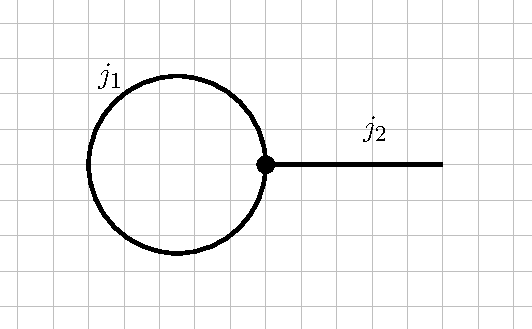
\includegraphics[width=69mm]{Graphs/1loop.pdf}
    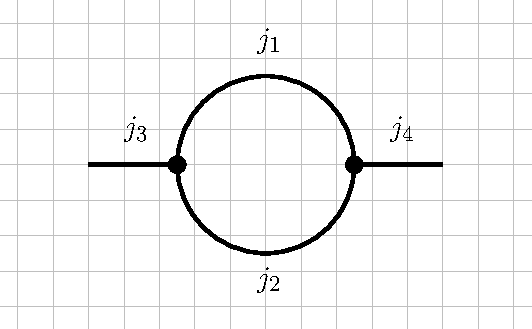
\includegraphics[width=69mm]{Graphs/2loop.pdf}
    \caption{Pictorial representation of the summation over projections. 3-$j$-symbols correspond to vertices, while angular momentum vectors are represented by edges. Left diagram corresponds to~\eqref{1loop}, where collapsing a 1-loop gives a factor of $\sqrt{(2j+1)}$, while the right diagram corresponds to~\eqref{2loop}, where collapsing a 2-loop produces a Kronecker delta function.}
    \label{fig:loops}
\end{figure}

\section{3j-symbols}
\label{app:3j}

Wigner 3-$j$ symbols are the coefficients with which three angular momenta must be added so that the resultant is zero. Most importantly for our purposes, they appear in the integral of three spherical harmonics~\eqref{3jInt}. For angular momentum vectors $j_1,j_2,j_3$ and their projections $m_1,m_2,m_3$, the 3-$j$ symbols are usually written in the form
\begin{equation}
    \begin{pmatrix} j_1 & j_2 & j_3 \\ m_1 & m_2 & m_3 \end{pmatrix}
\end{equation}
The closed-form expression evaluating a general 3-$j$ symbol is rather involved, but tabulate values can be found for example in~\cite{}. The necessary condition for a non-zero value are as follows:
\begin{itemize}
    \item $m_1+m_2+m_3 =0$,
    \item $j_1,j_2,j_3$ satisfy the triangle condition,
    \item $j_1+j_2+j_3$ is an integer (even integer if $m_1=m_2=m_3=0$).
\end{itemize}
Furthermore, permutation of any of the columns gives a factor of $(-1)^{j_1+j_2+j_3}$.

Summation over the projections in a product of 3-$j$ symbols can be conveniently represented graphically, with momenta $j$ represented by edges and 3-$j$ symbols by nodes. A shared edge denotes a shared value of $j$ with an opposite value of $m$. The summing over all $m$ then corresponds to collapsing subsequent loops in the resulting diagram. Each 1-loop gives a factor of $\sqrt{2j+1}$ and forces the remaining edge to be zero, while each 2-loop gives a Kronecker delta of the two outgoing edges. In the following we present the first few distinct cases. The sum over $m$ denotes summation over all $m_i$ indices..

Summing a single 3-$j$ symbol connected to itself, means collapsing a single 1-loop. The result is
\begin{equation}\label{1loop}
    \sum_m (-1)^{j_1-m_1}\begin{pmatrix} j_1 & j_1 & j_2 \\ -m_1 & m_1 & m_2\end{pmatrix} = \delta_{j_2,0}\sqrt{2j_1+1}.
\end{equation}
Summing over a pair of 3-$j$ symbols results in a product of two 1-loops or a single 2-loop:
\begin{align}
    &\sum_{m}(-1)^{m_1+m_2+m_3}
    \begin{pmatrix} j_1 & j_1 & j_3 \\ -m_1 & m_1 & -m_3 \end{pmatrix}
    \begin{pmatrix} j_2 & j_2 & j_4 \\ -m_2 & m_2 & m_4 \end{pmatrix} \nonumber
    \\
   & \mspace{250mu} = \delta_{j_3,0}\delta_{j_4,0}\sqrt{(2j_1+1)(2j_2+1)},\\
    &\sum_{m}(-1)^{m_1+m_2+m_3}
    \begin{pmatrix} j_1 & j_2 & j_3 \\ -m_1 & -m_2 & -m_3 \end{pmatrix}
    \begin{pmatrix} j_1 & j_2 & j_4 \\ m_1 & m_2 & m_4 \end{pmatrix}
    = \delta_{j_3,j_4}.\label{2loop}
\end{align}
The two situations~\eqref{1loop} and~\eqref{2loop} are presented in figure~\ref{fig:loops}. 

\begin{figure}
    \centering
    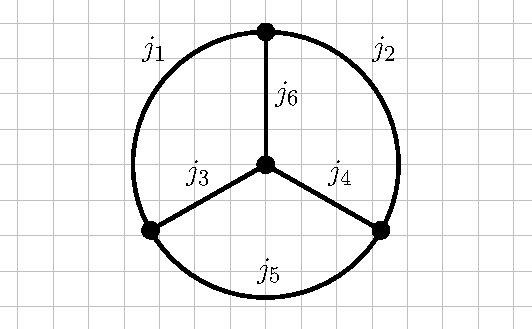
\includegraphics[width=69mm]{Graphs/6j.pdf}
    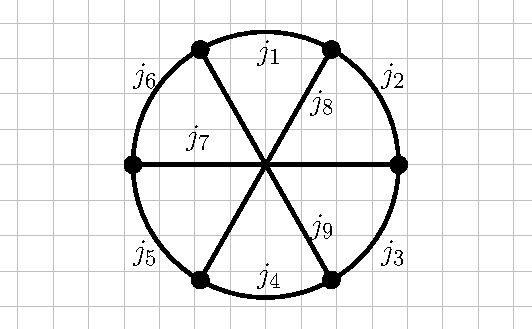
\includegraphics[width=69mm]{Graphs/9j.pdf}
    \caption{Pictorial representation of~\eqref{6j} resulting in a $6j-$symbol (left) and of~\eqref{9j}  resulting in a 9-$j$ symbol (right). In the right diagram there is no vertex in the middle\footnotemark. Notice that no 1-loops or 2-loops are present and so both of these do not simplify to combinations of Kronecker delta functions.}
    \label{fig:jsymbols}
\end{figure}
\footnotetext{There is no planar representation of such a graph, as it is isomorphic to the utility graph $K_{3,3}$~\cite{trudeau1993introduction}.}

Summation of three 3-$j$ symbols can always be performed by collapsing 1- and 2-loops, since the total number of legs is odd. The first non-trivial case happens with four interconnected 3-$j$ symbols in the form
\begin{align}\label{6j}
   \sum_m(-1)^\xi&\left(\begin{matrix}j_1&j_2&j_3\\-m_1&-m_2&-m_3\end{matrix}\right)\left(\begin{matrix}j_1&j_5&j_6\\m_1&-m_5&m_6\end{matrix}\right) \nonumber\\
   &\times\left(\begin{matrix}j_4&j_2&j_6\\m_4&m_2&-m_6\end{matrix}\right)\left(\begin{matrix}j_4&j_5&j_3\\-m_4&m_5&m_3\end{matrix}\right) =  \bigg\{\begin{matrix}j_1&j_2&j_3\\j_4&j_5&j_6\end{matrix}\bigg\}.
\end{align}
where $\xi = \sum_i (j_i-m_i)$. This quantity is called a 6-$j$ symbol for the purpose of tabulating values, as it does not reduce to a simple expression~\cite{biedenharn1984angular}. Similarly a product of 6 3-$j$ symbols can produce a 9-$j$ symbol
\begin{align}\label{9j}
   \sum_m(-1)^\xi&\left(\begin{matrix}j_1&j_2&j_3\\-m_1&-m_2&-m_3\end{matrix}\right)\left(\begin{matrix}j_4&j_5&j_6\\-m_4&-m_5&-m_6\end{matrix}\right) \nonumber\\
   &\mspace{50mu}\times\left(\begin{matrix}j_7&j_8&j_9\\-m_7&-m_8&-m_9\end{matrix}\right)\left(\begin{matrix}j_1&j_4&j_7\\m_1&m_4&m_7\end{matrix}\right) \nonumber
   \\
   &\mspace{50mu}\times\left(\begin{matrix}j_2&j_5&j_8\\m_2&m_5&m_8\end{matrix}\right)\left(\begin{matrix}j_3&j_6&j_9\\m_3&m_6&m_9\end{matrix}\right) =  \left\{\begin{matrix}j_1&j_2&j_3\\j_4&j_5&j_6\\j_7&j_8&j_9\end{matrix}\right\}.
\end{align}
Both of these are illustrated in figure~\ref{fig:jsymbols}. The exist  for evaluating the $6j-$ and 9-$j$ symbols can be performed with recursive algorithms analogous to the one used for 3-$j$ symbols~\cite{jsymbolsRef}.



\chapter{Evaluating Hypergeometric Functions}

\addtocontents{toc}{\contentsline
{chapter}{Appendix: Evaluating Hypergeometric Functions}{\protect\pageref{annotation}}}

	In this section we provide more technical details on evaluating the required hypergeometric functions, especially for the purpose of the convolution integral in the double-electron contribution to energy. It is generally difficult to find software capable of performing this accurately and efficiently, with all parameters being arbitrary complex numbers. One can use technical computing systems such as Mathematica, but these rely on arbitrary precission arithmetics, which is significantly less time-efficient, and details of the algorithms used are often not publicly available. For the purpose of producing the results presented here, we have written an original C++ library, designed specifically for the purpose of evaluating hypergeometric functions.
	
	\section{Confluent hypergeometric functions}
	
	Here we outline basic ideas used in developing our C++ library. First, let us note how the Whittaker functions appearing in the formula for hydrogen Green's function of arbitrary energy~\eqref{GreenESch} can be expressed by confluent hypergeometric functions \cite{AS}:
	\begin{equation}
M_{\kappa,\mu}(z) = e^{-\frac{z}{2}}z^{\mu + \frac{1}{2}}{_1F_1}(\mu-\kappa+\frac{1}{2},1+2\mu,z) ,
	\end{equation}
	\begin{equation}
	W_{\kappa,\mu}(z) = e^{-\frac{z}{2}}z^{\mu + \frac{1}{2}}U(\mu-\kappa+\frac{1}{2},1+2\mu,z) .
	\end{equation}

	Kummer's confluent hypergeometric function is defined for arbitrary complex numbers by a power series expansion:
		\begin{equation} \label{1F1}
		_1F_1(a,b,z) = \sum_i \frac{(a)_i}{(b)_i} \frac{z^i}{i!} ,
		\end{equation}
where $(a)_i$ is a Pochhamer symbol defined, as:
\begin{equation}
(a)_i = a(a+1)(a+2)...(a+i) .
\end{equation}

The series expansion (\ref{1F1}) is used to evaluate the confluent hypergeometric function in the region of small $|z|$, provided that the imaginary part of $a$ is also small. However, it has to be noted that it diverges whenever $b$ is a negative integer. Furthermore, truncating this series at desired accuracy requires considering the magnitude of two subsequent terms (as has been noted in \cite{Pearson2017}).

Confluent hypergeometric function satisfies the following differential equation (also referred to as confluent hypergeometric equation):
		\begin{equation}
		z \frac{d^2 w}{dz^2} + (b-z)\frac{dw}{dz} -a w = 0 ,
		\end{equation}
and can be defined as its solution analytic at $z=0$. The corresponding solution that diverges at 0 as $\propto z^{-a}$	is precisely the function $U(a,b,z)$.

\section{Algorithms for evaluating ${_1F_1}$}
		
		As noted above the defining power series is not always the optimal way of evaluating the confluent hypergeometric function. For large values of $|z|$ it is much more efficient to use the asymptotic expansion given by \cite{hazewinkel1993encyclopaedia}:
		\begin{equation}
		_1F_1(a,b,z) = \sum_i \frac{(a)_i (1+a-b)_i}{(i+1)!} \frac{-1}{z^i} .
		\end{equation}
		This is however a divergent series and therefore special care needs to be taken when determining when it should be truncated. The simple investigation of relative magnitudes of each component shows that terms in this sum only get smaller, as long as the term number is smaller than the modulus of the argument ($i<|z|$) and so it is not correct to go beyond this point even if more accuracy is desired.
			
		Furthermore, to limit critical cancellation it is convenient to ensure that $\text{Re}(z)>0$ by using the linear Kummers transformation \cite{AS}:
		\begin{equation}
		_1F_1(a,b,z) = e^z {_1F_1}(b-a,b,-z)
		\end{equation}
		
		The regime that causes the most problems is a large value of the imaginary part of $a$. There is however an approach that is often helpful in this case based on the expansion in terms of Bessel functions $J_{\nu}(z)$:		
		\begin{equation}
		_1F_1(a,b,z) = \Gamma(b) e^{\frac{z}{2}} 2^{b-1} \sum_i p_i(b,z) \frac{J_{b-1+j}(\sqrt{z(2b-4a)})}{[z(2b-4a)]^{\frac{1}{2}(b-1+j)}} ,
		\end{equation}
		where $p_n(a,x)$ is the nth Buchholz polynomial, defined in \cite{ABAD1999237}.
		
		Because of the oscillatory nature of Bessel functions, this approach should only be used when $|a|>|z|$. Otherwise, it is advantageous to revert to the original power series (\ref{1F1}).
		
		\section{Algorithms for evaluating U}
	
	The most straightforward way of evaluating the second confluent hypergeometric function is to relate it directly to {$_1F_1$}, by \cite{AS}:
		\begin{equation} \label{U}
		U(a,b,z) = \frac{\pi}{\sin(\pi b)}\frac{F(a,b,z)}{\Gamma(a-b+1)\Gamma(b)}-\frac{z^{1-b}}{\Gamma(a)\Gamma(2-b)!}F(1+a-b,2-b,z) ,
		\end{equation}
	which has to be understood as a limit if $a$ or $b$ are integers. When $b$ is a positive integer, the limit can be taken directly, to give:
	\begin{equation}
	U(a,b,z) = (-1)^a \frac{(a+b-1)!}{(b-1)!}{_1F_1(-a,b,z)} .
	\end{equation}
	
		On the other hand, when $b$ is a negative integer, we make use of another one of Kummer's transformations:
			\begin{equation}
			U(a,b,z) = z^{1-b}U(1+a-b,2-b,z) ,
			\end{equation}
		to make it positive and subsequently apply (\ref{U}).
		
	Finally, when $a$ is a negative integer, we repeatedly use the recurrence relation:
				\begin{equation}
				U(a,b,z) = -(b-2(a+1)-z)U(a+1,b,z)-(a+1)(2+a-b)U(a+2,b,z) ,
				\end{equation}
				until it can be expressed in terms of values of $U$ with a positive $a$ parameter.
						
			Extensive comparison of the above and many other formulas for evaluating confluent hypergeometric functions for a wide range of complex parameters can be found in \cite{Pearson2017}.


\end{appendices}

%\bibliographystyle{unsrt}
%\bibliographystyle{aipnum4-1}
%setcitestyle{numbers,square}
%\usepackage[sort&compress,numbers]{natbib}
%\bibliographystyle{apsrev4-1}
%\usepackage{doi}%<----------
%\usepackage{hyperref}

%\usepackage{hyperref}

%\bibliographystyle{apsrev4-1}
%\bibliographystyle{aipnum4-1}

%\usepackage[square,numbers]{natbib}
%\bibliographystyle{apsrev4-1}
%\setcitestyle{numbers}

\bibliography{Thesis.bib}

\chapter*{Acknowledgement}

I would like to thank everyone who contributed, directly and indirectly to this work. First and foremost, Dr. Oleg Skoromnik, who started this research, for all his help and patience in guiding me through the early stages of my project. Secondly, my supervisors PD Dr. Natalia S Oreshkina and Honorarprofessor Dr. Christoph H Keitel for the expertise and support in completing this thesis. Finally, Dominik Lentrodt and Dr. Halil Cakir for help with translating the abstract, as well as Michael Quin, Dr. Daniel Bakucz-Can\'ario and PD Dr. Zolt\'an Harman for proofreading the manuscript and helpful discussions. Last but not least, all my other friends and colleagues at MPIK for all the help and fun times together.

I would also like to thank Prof. Dr. Joerg Jaeckel for kindly agreeing to review my thesis, as well as PD Dr. Robert Moshammer and Prof. Dr. Kurt Roth for agreeing to participate in my defense.

\end{document}


%1 - written roughly/coppied
%2 - written in a thoughtfull/original way
%3 - inlcudes input from Natalia
%4 - more or less in a final form
%5 - finished
%6 - corrected commas/grammar